%Version 3.1 December 2024
% See section 11 of the User Manual for version history
%
%%%%%%%%%%%%%%%%%%%%%%%%%%%%%%%%%%%%%%%%%%%%%%%%%%%%%%%%%%%%%%%%%%%%%%
%%                                                                 %%
%% Please do not use \input{...} to include other tex files.       %%
%% Submit your LaTeX manuscript as one .tex document.              %%
%%                                                                 %%
%% All additional figures and files should be attached             %%
%% separately and not embedded in the \TeX\ document itself.       %%
%%                                                                 %%
%%%%%%%%%%%%%%%%%%%%%%%%%%%%%%%%%%%%%%%%%%%%%%%%%%%%%%%%%%%%%%%%%%%%%

%%\documentclass[referee,sn-basic]{sn-jnl}% referee option is meant for double line spacing

%%=======================================================%%
%% to print line numbers in the margin use lineno option %%
%%=======================================================%%

%%\documentclass[lineno,pdflatex,sn-basic]{sn-jnl}% Basic Springer Nature Reference Style/Chemistry Reference Style

%%=========================================================================================%%
%% the documentclass is set to pdflatex as default. You can delete it if not appropriate.  %%
%%=========================================================================================%%

%%\documentclass[sn-basic]{sn-jnl}% Basic Springer Nature Reference Style/Chemistry Reference Style

%%Note: the following reference styles support Namedate and Numbered referencing. By default the style follows the most common style. To switch between the options you can add or remove “Numbered” in the optional parenthesis. 
%%The option is available for: sn-basic.bst, sn-chicago.bst%  
 
%%\documentclass[pdflatex,sn-nature]{sn-jnl}% Style for submissions to Nature Portfolio journals
%%\documentclass[pdflatex,sn-basic]{sn-jnl}% Basic Springer Nature Reference Style/Chemistry Reference Style
\documentclass[pdflatex,sn-mathphys-num]{sn-jnl}% Math and Physical Sciences Numbered Reference Style
%%\documentclass[pdflatex,sn-mathphys-ay]{sn-jnl}% Math and Physical Sciences Author Year Reference Style
%%\documentclass[pdflatex,sn-aps]{sn-jnl}% American Physical Society (APS) Reference Style
%%\documentclass[pdflatex,sn-vancouver-num]{sn-jnl}% Vancouver Numbered Reference Style
%%\documentclass[pdflatex,sn-vancouver-ay]{sn-jnl}% Vancouver Author Year Reference Style
%%\documentclass[pdflatex,sn-apa]{sn-jnl}% APA Reference Style
%%\documentclass[pdflatex,sn-chicago]{sn-jnl}% Chicago-based Humanities Reference Style

%%%% Standard Packages
%%<additional latex packages if required can be included here>

\usepackage{graphicx}%
\usepackage{multirow}%
\usepackage{amsmath,amssymb,amsfonts}%
\usepackage{amsthm}%
\usepackage{mathrsfs}%
\usepackage[title]{appendix}%
\usepackage{xcolor}%
\usepackage{textcomp}%
\usepackage{manyfoot}%
\usepackage{booktabs}%
\usepackage{bm}% for bold math symbols
\usepackage{algorithm}%
\usepackage{algorithmicx}%
\usepackage{algpseudocode}%
\usepackage{listings}%
\lstset{upquote=false,basicstyle=\fontencoding{T1}\selectfont}
\usepackage{tabularx}
\usepackage[caption=false]{subfig}
%\usepackage[hidelinks]{hyperref}
\usepackage{comment}

%\newcommand\red[1]{{\color{red}#1}}
\newcommand\red[1]{#1}
%\newcommand\redb[1]{{\color{red}#1}}
\newcommand\redb[1]{#1}
%\newcommand\redc[1]{{\color{red}#1}}
\newcommand\redc[1]{#1}
%\newcommand\blue[1]{{\color{blue}#1}}
\newcommand\blue[1]{#1}
%%%%

%%%%%=============================================================================%%%%
%%%%  Remarks: This template is provided to aid authors with the preparation
%%%%  of original research articles intended for submission to journals published 
%%%%  by Springer Nature. The guidance has been prepared in partnership with 
%%%%  production teams to conform to Springer Nature technical requirements. 
%%%%  Editorial and presentation requirements differ among journal portfolios and 
%%%%  research disciplines. You may find sections in this template are irrelevant 
%%%%  to your work and are empowered to omit any such section if allowed by the 
%%%%  journal you intend to submit to. The submission guidelines and policies 
%%%%  of the journal take precedence. A detailed User Manual is available in the 
%%%%  template package for technical guidance.
%%%%%=============================================================================%%%%

%% as per the requirement new theorem styles can be included as shown below
\theoremstyle{thmstyleone}%
\newtheorem{theorem}{Theorem}%  meant for continuous numbers
%%\newtheorem{theorem}{Theorem}[section]% meant for sectionwise numbers
%% optional argument [theorem] produces theorem numbering sequence instead of independent numbers for Proposition
\newtheorem{proposition}[theorem]{Proposition}% 
%%\newtheorem{proposition}{Proposition}% to get separate numbers for theorem and proposition etc.

\theoremstyle{thmstyletwo}%
\newtheorem{example}{Example}%
\newtheorem{remark}{Remark}%

\theoremstyle{thmstylethree}%
\newtheorem{definition}{Definition}%

\raggedbottom
%%\unnumbered% uncomment this for unnumbered level heads

\begin{document}

\title[LodusPop: Environment-Driven Urban Population Simulation]{LodusPop: An Environment-Driven Multi-Scale Simulation Framework for Urban Population Dynamics, Service Resilience, and Flood-Aware Mobility}

%%=============================================================%%
%% GivenName	-> \fnm{Joergen W.}
%% Particle	-> \spfx{van der} -> surname prefix
%% FamilyName	-> \sur{Ploeg}
%% Suffix	-> \sfx{IV}
%% \author*[1,2]{\fnm{Joergen W.} \spfx{van der} \sur{Ploeg} 
%%  \sfx{IV}}\email{iauthor@gmail.com}
%%=============================================================%%

\author*{\fnm{Gabriel} \sur{Fonseca Silva}}\email{fonseca.gabriel@pucrs.br}

\author[1]{\fnm{André} \sur{da Silva Antonitsch}}\email{andre.antonitsch@edu.pucrs.br}
%\equalcont{These authors contributed equally to this work.}

\author{\fnm{Soraia} \sur{Raupp Musse}}\email{soraia.musse@pucrs.br}
%\equalcont{These authors contributed equally to this work.}

\affil*{\orgdiv{Virtual Humans Laboratory (VHLab) - School of Tecnology}, \orgname{Pontifical Catholic University of Rio Grande do Sul (PUCRS)}, \orgaddress{\street{Av. Ipiranga, 6681 - Partenon}, \city{Porto Alegre}, \postcode{ 90619-900}, \state{RS}, \country{Brazil}}}

%%==================================%%
%% Sample for unstructured abstract %%
%%==================================%%

\abstract{Urban population simulations can support the comparison of planning and emergency-response alternatives, but many approaches require detailed individual trajectories or remain tied to one application domain. This thesis presents LodusPop, an environment-driven, multi-scale simulation framework in which locations request population flows and populations are represented as heterogeneous blobs that can split, merge, move, and change state. The framework is extended with dynamic node availability and dependency constraints while retaining domain behavior in plugins. Its applicability is examined through published mobility, large-event, and epidemic studies and through new experiment families concerning inpatient care, dialysis-service disruption, routine activity visits, flooding, destination adaptation, and flood-aware commuting in Porto Alegre, Brazil. The experiments use both neighborhood-level and census-sector home representations, repeated and matched random seeds where appropriate, and domain-specific conservation and integrity checks. Results show how service coverage depends on capacity, spatial distribution, recovery time, and infrastructure dependencies, while flood experiments distinguish activity visits that can be rerouted from work and school trips with less substitutable destinations. Complementary immersive and origin--destination visualizations illustrate ways to inspect simulation outputs, but are not treated as behavioral validation. The results are comparative outcomes under explicit assumptions rather than forecasts. Together, the studies demonstrate that LodusPop supports a broad family of auditable urban population scenarios without promoting application-specific capacities, queues, or adaptation rules into the core population model.}

% The results highlight LodusPop as a practical and extensible tool for urban planning, crisis management, and public health interventions, bridging the gap between data availability, computational scalability, and the ability to analyze population dynamics across multiple spatial and temporal scales.


%%================================%%
%% Sample for structured abstract %%
%%================================%%

% \abstract{\textbf{Purpose:} The abstract serves both as a general introduction to the topic and as a brief, non-technical summary of the main results and their implications. The abstract must not include subheadings (unless expressly permitted in the journal's Instructions to Authors), equations or citations. As a guide the abstract should not exceed 200 words. Most journals do not set a hard limit however authors are advised to check the author instructions for the journal they are submitting to.
% 
% \textbf{Methods:} The abstract serves both as a general introduction to the topic and as a brief, non-technical summary of the main results and their implications. The abstract must not include subheadings (unless expressly permitted in the journal's Instructions to Authors), equations or citations. As a guide the abstract should not exceed 200 words. Most journals do not set a hard limit however authors are advised to check the author instructions for the journal they are submitting to.
% 
% \textbf{Results:} The abstract serves both as a general introduction to the topic and as a brief, non-technical summary of the main results and their implications. The abstract must not include subheadings (unless expressly permitted in the journal's Instructions to Authors), equations or citations. As a guide the abstract should not exceed 200 words. Most journals do not set a hard limit however authors are advised to check the author instructions for the journal they are submitting to.
% 
% \textbf{Conclusion:} The abstract serves both as a general introduction to the topic and as a brief, non-technical summary of the main results and their implications. The abstract must not include subheadings (unless expressly permitted in the journal's Instructions to Authors), equations or citations. As a guide the abstract should not exceed 200 words. Most journals do not set a hard limit however authors are advised to check the author instructions for the journal they are submitting to.}

\keywords{Environment-driven simulation, Multi-scale modeling, Human mobility, Health-service resilience, Flood-aware mobility, Urban population dynamics}

%%\pacs[JEL Classification]{D8, H51}

%%\pacs[MSC Classification]{35A01, 65L10, 65L12, 65L20, 65L70}

\maketitle

\section{Introduction}
\label{sec:introduction}

\subsection{Motivation and Problem}

Recent crises have underscored the critical role of population modeling in urban planning and crisis management. Cities worldwide have faced urgent challenges in managing mobility, enforcing social distancing measures, and regulating the use of public spaces such as malls, supermarkets, and health services\citep{shafiri2020covidImpact, kang2021hybridCovid, bouchnita2021mathModelCovid}. Similar challenges also emerge in other contexts, including disaster response, large-scale events, and climate-related risks\citep{eid1980, tekouabou2022MLinUrbanPlanning, haraguchi2022mobilityDataReview, serana2023multilevelmodeling}. These scenarios highlight the importance of simulation systems that can \redb{support the evaluation of urban policies and decisions}, providing insights into how individuals and groups interact with the built
environment\citep{kang2021hybridCovid, tekouabou2022MLinUrbanPlanning}.

Simulation models are central to supporting evidence-based urban planning, from optimizing public transportation and allocating residential areas to improving the overall resilience of city systems~\citep{eid1980, tekouabou2022MLinUrbanPlanning}. Human mobility is particularly relevant, forming the basis of research in epidemic control, traffic simulation, and socio-economic studies~\citep{haraguchi2022mobilityDataReview, serana2023multilevelmodeling}. Existing methods span microscopic approaches that track individual agents~\citep{helbing1995social, cao2021competitiveCooperative, khan2024heterogeneousSurvey, ruprecht2024adaptiveMovement}, macroscopic approaches that capture aggregated flows~\citep{hughes2002continuum, treuille2006continuum,thalmann2007crowd}, and hybrid models that combine both perspectives~\citep{xiong2010hybrid, ijaz2015hybridSurvey, antonitsch2019bioclouds, dang2023multilevelCrowd}. 
%Despite these advances, two major challenges remain: i) Integration across scales: connecting individual-level routines with population-wide patterns in a consistent framework~\citep{cogo2019integrability, alessandretti2020nature}; ii) Dependence on detailed data: most population-driven models rely on granular behavioral or mobility data, which is often unavailable or impractical to collect due to privacy and scalability concerns~\citep{cogo2019integrability, alessandretti2020nature}.
\redb{In this thesis, our focus is on urban population modeling and mobility-oriented simulations across these scales, rather than on high-fidelity, collision-level crowd simulation.} Despite the significant advances of existing methods, two major challenges remain for such population-dynamics platforms: i) integration across scales—connecting individual-level routines with population-wide patterns in a consistent framework~\citep{cogo2019integrability, alessandretti2020nature}; and ii) dependence on detailed data—most population-driven models rely on granular behavioral or mobility data, which is often unavailable or impractical to collect due to privacy and scalability concerns~\citep{cogo2019integrability, alessandretti2020nature}.

\subsection{Research Gap}

Beyond routine mobility, an urban simulator intended for comparative planning must represent changes in the environment itself. A clinic may close, a home or point of interest may become exposed to floodwater, and the failure of a water-treatment facility may make dependent services unavailable. The population response also varies by domain: one trip may be suppressed, another may wait for capacity, and another may be redirected to a safe alternative. Existing mobility and service simulations frequently embed such assumptions in a domain-specific model, limiting reuse and obscuring the boundary between the general simulation mechanism and the policy being tested.

This thesis therefore considers a third challenge in addition to integration across scales and dependence on detailed data: representing availability, capacity, disruption, and adaptation through explicit extensions while preserving a stable population model. Dynamic node availability and dependency constraints are treated as general properties of the environment. Health-service queues, flood exposure, destination substitution, and commute recovery remain plugin policies and, consequently, visible scenario assumptions.

% Paragrafo sugerido pelo nosso amigo
%\redb{Traditional microscopic crowd simulation approaches concentrate on detailed agent-level decision processes and collision avoidance, whereas population mobility models emphasize large-scale statistical patterns and flows inferred from data such as mobile-phone traces or surveys. Our goal with LodusPop is not to replicate high-fidelity microscopic crowd behavior, but to provide a macro- and meso-scale population-dynamics platform. By operating primarily at the level of aggregated population units and allowing environments to request movements, the framework is geared toward questions such as how different opening hours, zoning rules, or vaccination strategies affect the occupancy of key locations over time, rather than toward precise path-level validation at the individual scale.}

To address these challenges, we introduce LodusPop, a flexible framework for simulating urban populations across multiple spatial and temporal scales. \redb{Instead of focusing on individual decision-making and detailed trajectory planning, LodusPop targets macro- and meso-scale population dynamics: environments actively request movements from aggregated population units.} This environment-driven paradigm reduces reliance on fine-grained data while still capturing key patterns in aggregate flows and occupancy. Populations are represented through blobs -- arbitrarily sized groups of individuals with defined attributes and routines -- that can split, merge, and evolve during a simulation. This abstraction balances computational efficiency with the ability to represent heterogeneous population behaviors across scales ranging from neighborhoods to entire cities, while still providing hooks for micro-style routines when localized detail is needed.

\subsection{Research Questions and Objectives}

The general objective is to develop and evaluate a reusable framework for modeling heterogeneous urban populations under routine conditions, policy interventions, capacity limits, and environmental disruption. The thesis is organized around four research questions:

\begin{description}
    \item[RQ1:] How can an environment-driven, blob-based representation express heterogeneous population dynamics at neighborhood and census-sector spatial granularities?
    \item[RQ2:] How can plugins, dynamic node availability, and dependency constraints represent domain-specific capacity, disruption, and adaptation while preserving a stable core model?
    \item[RQ3:] What does the application of this common framework to mobility, public-health, health-service, and flood scenarios demonstrate about its versatility and practical limits?
    \item[RQ4:] Which provenance, replication, validation, and visualization practices are necessary to interpret the generated outcomes as auditable scenario comparisons rather than forecasts?
\end{description}

To answer these questions, this thesis defines the LodusPop environment, population, and routine abstractions; retains the published experiments on random movement, large-scale events, epidemic contagion, vaccination, and computational performance; and extends the evaluation with inpatient-care, dialysis-service, routine-activity, flood, destination-adaptation, and flood-aware commute experiments. Complementary visualization studies examine how aggregate outputs can be inspected without being confused with behavioral validation.

%To address these limitations, we introduce LodusPop, a flexible framework for simulating urban populations across multiple spatial and temporal scales. Instead of focusing on individual decision-making, LodusPop employs an environment-driven paradigm, where environments actively request movements from populations. This inversion of responsibility reduces reliance on fine-grained data while still capturing realistic dynamics. Populations are represented through blobs—arbitrarily sized groups of individuals with defined attributes and routines—that can split, merge, and evolve during a simulation. This abstraction balances computational efficiency with the ability to represent heterogeneous population behaviors across scales ranging from neighborhoods to entire cities.

\subsection{Thesis Contributions}

\blue{
The main contributions of this thesis are as follows:
\begin{itemize}
    \item We propose an environment-driven modeling paradigm that shifts decision-making from individuals to the environment, \redb{reducing data requirements while remaining suitable for multi-scale urban mobility and policy analysis.}
    \item We introduce the blob abstraction, enabling flexible and scalable representation of populations that adapt to data availability and simulation needs.
    \item \redb{We design LodusPop, a multi-scale simulation framework that integrates GIS-based environments with a blob-based population model within a unified architecture.}%We design LodusPop, a multi-scale simulation framework that integrates GIS-based environments, agent-based micro-dynamics, and macro-level models within a unified architecture.}
    \item We extend the environment with cause-aware node availability and dependency constraints, allowing direct disruption, recovery, and cascading service unavailability to be represented consistently.
    \item We evaluate LodusPop through cumulative case studies in Porto Alegre covering routine mobility, large-scale events, epidemic control, inpatient and dialysis services, flooding, destination adaptation, and commuting.
    \item We synthesize immersive and origin--destination visualization approaches, clarifying their role in exploring rather than validating simulation outcomes.
\end{itemize}

Together, these contributions establish LodusPop as a practical and extensible framework for studying urban population dynamics. The generated results are comparisons between explicitly modeled scenarios; they are not forecasts of individual behavior, clinical demand, or future flood impacts.}

\begin{comment}
    

The COVID-19 pandemic underscored the critical role of population modeling in strategic planning\citep{shafiri2020covidImpact}. Cities worldwide faced the urgent need to manage social distancing, regulate mobility, and impose limits on the use of public spaces such as malls, supermarkets, and health services. These challenges highlighted the importance of simulation systems capable of realistically evaluating policies and decisions in urban environments, as they provide insights into how individuals and groups interact with the built environment\citep{kang2021hybridCovid, bouchnita2021mathModelCovid}.

Simulation systems play a pivotal role in providing data for informed decision-making in urban planning, such as optimizing public transportation, allocating residential areas, and improving overall city flow~\citep{eid1980, tekouabou2022MLinUrbanPlanning}. Human mobility serves as a foundation for diverse research domains, including epidemic modeling, traffic simulation, and socio-economic studies~\citep{haraguchi2022mobilityDataReview, serana2023multilevelmodeling}. Urban mobility simulation methods span from modeling traffic dynamics in large metropolitan areas~\citep{ng2017trafficSim, garg2019traffic3d} to analyzing pedestrian movements in confined spaces~\citep{mather2019walkability, hassannayebi2020hybridEvacuation,liu2022optimizationEvacuationShip}. Hybrid models have also emerged, combining micro- and macroscopic perspectives to simulate populations in a unified environment~\citep{xiong2010hybrid, ijaz2015hybridSurvey, antonitsch2019bioclouds, dang2023multilevelCrowd}.

Still, a challenge that the modeling of virtual urban environments presents is the integration between data to describe structures at different levels of a city's hierarchy and the different scales present in human mobility~\citep{cogo2019integrability, alessandretti2020nature}. Traditional approaches to population simulations often rely on individuals or groups making decisions based on granular behavioral data, such as preferences or probabilistic rules. While effective in some contexts, these population-driven models present significant challenges, particularly when detailed data on individual movements and locations is unavailable or incomplete due to privacy concerns, collection limitations, or scalability issues.

This work introduces a model for simulating populations and their behaviors within multi-level detail environments. It leverages crowd simulation strategies, particularly the abstraction of individuality inherent in macroscopic simulation models~\citep{antonitsch2019bioclouds,legion}. The model emphasizes representing groups of individuals, regardless of size, to simulate population mobility across environments of varying scales, from city blocks to entire cities, counties, or states.
Additionally, we present a novel environment-driven approach, where the environment actively requests movements from the population. By reversing the traditional paradigm, this method minimizes reliance on granular individual-level data, instead leveraging aggregated or generalized information about population distributions and environmental needs.

\red{The main contributions of this paper lie in the development of LodusPop, a multi-scale population simulation framework.} % designed as the population layer for the existing LODUS framework~\citep{silva2020lodus}. 
LodusPop introduces a novel approach by modeling populations as arbitrarily sized ``blobs'', each endowed with specific population characteristics and routines, allowing for dynamic adaptation of simulation granularity based on data availability and modeling needs. This flexibility holds significant promise for computational efficiency and enhanced decision-making. Additionally, the paper demonstrates the applicability of LodusPop through three diverse case studies focused on urban dynamics in Porto Alegre, Brazil, showcasing the utility of a single, consistent population model across various phenomena.
\end{comment}

\subsection{Publications and Thesis Organization}

The model and original experiment family are based on the \textit{main\_submission} manuscript. The inpatient-care lineage and hospital-capacity data originate in the LODUS-Health master's dissertation by Souza~\citep{souza2026lodushealth}; the recent batches reported here are separate experiments and are not a republication of that dissertation's results. The immersive visualization is collaborative published work~\citep{teixeira2024visualization}, whereas the geographic flow tool is student-led work developed by Silva under the supervision of the thesis author~\citep{silva2026geospatial}. These sources are integrated with explicit attribution and with a distinction between prior artifacts, recent simulation work, and the synthesis contributed by this thesis.

Section~\ref{sec:related_work} reviews crowd, mobility, resilience, health-service, flood, and visualization research. Section~\ref{sec:proposed_model} defines the LodusPop framework and its extension boundary. Section~\ref{sec:extended_evaluation} establishes the shared evaluation design and Porto Alegre case context. The evidence then follows a capability progression: routine mobility and spatial granularity in Section~\ref{sec:routine_mobility}; demand shocks and population-state interventions in Section~\ref{sec:interventions}; environmental disruption and destination adaptation in Section~\ref{sec:flood_mobility}; and health and critical-service resilience in Section~\ref{sec:health_resilience}. Section~\ref{sec:computational_analysis} brings together the published computational evaluation and supporting visualization work. Section~\ref{sec:discussion} synthesizes the evidence and limitations, and Section~\ref{sec:conclusion} concludes the thesis. Detailed input and simulator examples remain in Appendix~\ref{app:input}.



\section{Related Work}
\label{sec:related_work}

\blue{Research on modeling population dynamics spans two central but historically distinct areas: crowd simulation and population mobility modeling. Crowd simulation emphasizes fine-grained representations of movement and interactions among individuals or groups, whereas population mobility focuses on larger-scale flows and statistical regularities in urban dynamics. Each domain has produced significant advances, but both exhibit limitations that motivated the development of LodusPop.}

\subsection{Crowd Simulation}
\label{related:crowd_simulation}
\blue{
Crowd simulation has long served as a foundation for understanding human movement in both indoor and outdoor environments, with models developed at microscopic, macroscopic, and hybrid scales.

Microscopic models treat every agent as an autonomous entity with decision-making capabilities\redb{, typically influenced by local environmental conditions}. Classical examples include the Social Force Model~\citep{helbing1995social}, where pedestrian motion emerges from forces balancing personal goals with environmental and social interactions, and ORCA~\citep{van2011reciprocal}, which guarantees collision-free trajectories through reciprocal velocity obstacles. BioCrowds~\citep{de2012simulating} introduced a space-discretization strategy where agents compete for territory, naturally generating emergent Voronoi-like partitions. Later studies aimed to add heterogeneity by embedding psychological or emotional states into agent behavior. For example, Pelechano et al.~\citep{pelechano2005crowd} and Durupinar et al.~\citep{durupinar2015psychological} integrated factors such as stress, emotion, and cultural variation, while Neto et al.~\citep{neto2017giving} modeled emotional contagion based on personality traits. These approaches achieve remarkable behavioral variety, but they depend heavily on detailed behavioral datasets and quickly become computationally expensive when scaled up to large urban populations.

In contrast, macroscopic models treat crowds as collective entities, often described through density fields or flow equations. Hughes~\citep{hughes2002continuum} and Treuille et al.~\citep{treuille2006continuum} pioneered continuum models where population density evolves through potential fields\redb{ defined over the environment, while proposed Antonitsch et al.~\citep{antonitsch2019bioclouds} BioClouds,
aggregating agents into homogeneous “clouds” competing for space based on density
and velocity preferences. Such formulations shift
part of the steering to environment-side representations and significantly improve computational scalability,} but they sacrifice the diversity of individual behaviors.

Hybrid models attempt to combine these two perspectives. For example, Legion\citep{legion} dynamically adapts the level of detail based on environmental complexity, allowing legions of agents to split or merge as situations demand. Xiong et al.~\citep{xiong2010hybrid} proposed spatially partitioned hybrid simulations that combine ORCA~\citep{van2011reciprocal} in high-interest regions with continuum models elsewhere, while Lemonari et al.~\citep{lemonari2025mpact} introduced MPACT, a mesoscopic framework that uses learned profiles to capture intermediate-scale behaviors. \redb{These hybrids achieve flexibility, however, the primary focus of
control remains on the population side. Agents query these fields and detailed data is often required for accurate calibration.}% but they remain fundamentally population-driven: individuals or groups still determine their own movements, and detailed data is required for accurate calibration.

\redb{Recent advances explore ways to alleviate this dependency through data-driven modeling, where behavior is learned from observed or simulated trajectories rather than being entirely hand-crafted. For instance, machine learning has been used to embed agent dynamics into low-dimensional manifolds, enabling multiscale reconstruction of crowd flows~\citep{alvarez2025quationfree}. 
Deep reinforcement learning approaches, such as those proposed by Li et al.~\citep{Li2025efficienteCrowdSim}, combine learned navigation strategies with anisotropic environmental fields to reduce computational costs in large spaces. 
In many of these studies, policies are learned from large numbers of simulated episodes rather than from real mobility datasets. Behavior is governed by fitted models whose data requirements center on simulated experience rather than fine-grained observational traces, and the underlying agent-based perspective remains unchanged.}%While promising, these methods still require rich datasets and do not fundamentally change the agent-centric paradigm.

In summary, crowd simulation excels in behavioral realism and the reproduction of fine-scale interactions. However, the reliance on detailed micro-data and high computational costs make it difficult to deploy at the scale of entire cities or to apply when granular behavioral data is unavailable.
}

\begin{comment}
Crowd simulation techniques are commonly used to represent the movement of a population, both in interior and exterior environments and in various levels of detail, including microscopic points of view~\citep{helbing1995social, pelechano2005crowd, narang2015generating, cao2021competitiveCooperative, zhang2023collectiveBehavior}; macroscopic points of view~\citep{hughes2002continuum, treuille2006continuum}; and a combination of both (i.e., hybrid)~\citep{antonitsch2019bioclouds}. 

% Microscopic models with homogeneous behaviors
In microscopic crowd simulation models, each agent in a crowd is a single entity of simulation\citep{macal2010agentBasedTutorial, xiong2014motionPlanning}. Some models propose homogeneous behaviors ~\citep{helbing1995social, van2011reciprocal, de2012simulating}, where agents will behave similarly to each other and show little to no individuality. 
Helbing and Molnár~\citep{helbing1995social} presented the Social Forces Model, where agent movement is influenced by their desired velocity toward a destination, distance from other agents, and interaction with the environments (e.g., obstacles and walls). 
ORCA (Optimal Reciprocal Collision Avoidance), proposed by Van den Berg et al.~\citep{van2011reciprocal}, simulates agents based on reciprocal velocity obstacles (RVO).
BioCrowds, presented by Bicho et al.~\citep{de2012simulating}, proposes a space discretization and competition model for crowd simulation, where agents compete to maintain their personal space by taking possession of space around them, forming an emergent Voronoi partitioning of space. A collision-free movement is guaranteed if no agent attempts to move outside its individual space.

% Microscopic models with heterogeneous behaviors (could be removed/reduced/combined with previous paragraph)
There has been research on how to model heterogeneous behavior for individual agents in crowds.
Pelechano et al.~\citep{pelechano2005crowd} proposed a model to incorporate psychological aspects and communication into crowd simulations to generate emergent cultural behavior. The authors model human behavior like stress, emotion, motivation, decision process, and ability, impacting decision-making under the agent's varied emotional state (e.g., stress levels and physiological state).
Durupinar et al.~\citep{durupinar2015psychological} proposed a model to differentiate crowds between audiences and mobs as passive and active crowds, respectively, influenced by emotional and homogeneous behavior. Authors present an emotion contagion model based on OCEAN personality traits (\textit{Openness}, \textit{Conscientiousness}, \textit{Extroversion}, \textit{Agreeableness} and \textit{Neuroticism}), employing the OCC emotion model in multi-agent simulations, and utilizing a pleasure-arousal-dominance (PDA) model do influence agent decision-making.
Neto et al.~\citep{neto2017giving} propose a model based on BioCrowds~\citep{de2012simulating} to simulate the spread of psychological phenomena in a crowd of virtual agents. Agents are imbued with OCEAN personality traits and emotional information and can spread that information based on factors such as expressiveness, susceptibility to contagion, and current goal.


% Macroscopic models
In macroscopic crowd simulation models, agents are represented as part of a collective being controlled or influenced by a macro-level structure~\citep{thalmann2007crowd}, e.g., density fields or aggregations of agents. This allows a higher granularity and smaller simulation cost with a trade-off of losing individual characteristics and behaviors for each agent. 
Treuille et al.~\citep{treuille2006continuum} proposed the Continuum Crowds model, which is based on continuum field dynamics and inspired by the work of Hughes~\citep{hughes2002continuum}. The authors simulate a crowd as a dynamic potential field to perform navigation for agents and moving obstacles without explicit agent-based dynamics. 
Antonitsch et al.~\citep{antonitsch2019bioclouds} presented BioClouds, based on BioCrowds~\citep{de2012simulating}, which models crowds as a set of clouds. Each cloud comprises a group of agents with a similar desire for a specific density, speed, and goal. Clouds compete for space amongst each other and occupy the environment in a manner that tries to keep their desired densities respected. 

% Hybrid models
Hybrid approaches for crowd simulation have also been proposed, combining distinct microscopic and macroscopic models and leveraging the accuracy and computational efficiency. Xiong et al.~\citep{xiong2010hybrid} suggest separating the environment into static regions. Regions of interest are simulated with ORCA~\citep{van2011reciprocal}, and the remaining space with Continuum Crowds~\citep{treuille2006continuum}. The regions are interfaced with transition regions, with agents that cross these boundaries being removed from one simulation and added to the other. 
BioClouds~\citep{antonitsch2019bioclouds} also presents a way to transition between macroscopic and microscopic simulations. The authors utilize a visualization window that covers a region in the environment. The area within this region and agents of clouds that occupy it are simulated with the BioCrowds~\citep{de2012simulating} model.
Legion, proposed by Antonitsch et al.\citep{legion}, presents a crowd simulation model where the simulation dynamically changes the level of detail of the modeled agents according to environment complexity. A legion (i.e., crowds of people) may split into smaller groups whenever it's in a situation where it would occupy less space than desired in a future frame, e.g., moving towards an obstacle. Different legions may also merge when they share the same objective and are close enough to regroup.
\red{
Lemonari et al.~\citep{lemonari2025mpact} propose MPACT, a mesoscopic crowd simulation framework that transforms unlabelled trajectory data into interpretable behavior profiles using image-based encodings. Unlike traditional microscopic or macroscopic models, MPACT operates at an intermediate level, capturing group dynamics and localized interactions. Trained on synthetic data, its predictive model maps spatial encodings to high-level simulator parameters, enabling behavior-driven simulations without manual tuning.}
\end{comment}

\subsection{Population Mobility}

\blue{Population mobility studies emerged from statistical and large-scale analyses of human movement patterns. Unlike crowd simulation, which centers on the agent, mobility modeling typically abstracts away individuality to emphasize flows across geographic space and time.

A consistent finding in this field is that human displacements follow heavy-tailed distributions. Brockmann et al.~\citep{brockmann2006scaling} showed that the circulation of banknotes in the United States resembled Lévy flights, while González et al.~\citep{gonzalez2008understanding}, analyzing cell phone data, demonstrated that most individuals repeatedly visit a small set of locations. Song et al. ~\citep{natureSong2010exploration}  formalized this as a combination of exploration (discovering new places) and preferential return (frequent revisits), and Alessandretti et al.~\citep{alessandretti2020nature} refined these ideas with hierarchical ``containers'', arguing that people conceptualize space in nested levels such as neighborhoods, cities, and regions. These statistical regularities provide strong predictive power, but they are generally limited to describing long-term patterns rather than simulating short-term interventions or local policies.

The COVID-19 pandemic highlighted the importance of connecting mobility with public health. Studies such as Jamshidi et al.~\citep{jamshidi2020global} examined the effect of density and mobility restrictions on infection rates, while Hernández-Orallo et al.~\citep{hernandez2021human} used urban simulations to identify risk hotspots like train stations and plazas. Kraemer et al.~\citep{natureKramer2020mobilityCovid} quantified how mobility and control measures influenced epidemic spread in China. These works demonstrated the societal relevance of mobility modeling but remained largely domain-specific, oriented toward epidemiology rather than more general urban planning applications.

Frameworks for simulating mobility have also emerged. Silva et al.~\citep{silva2020lodus} introduced a framework that integrates environmental data with macroscopic BioClouds to simulate contagion scenarios. Although innovative, its reliance on homogeneous clouds and a narrow focus on epidemics limited its applicability. More recent frameworks increasingly incorporate machine learning and multi-scale techniques [6,7,16], but they remain strongly tied to data availability and typically adhere to the population-driven logic of traditional mobility models.

Recent contributions push the field toward more interpretable, adaptable, and AI-enhanced approaches. Liu et al.~\citep{liu2024GraviGBM} proposed GraviGBM, which blends gravity-based migration models with gradient-boosted machine learning, balancing predictive accuracy and interpretability. Other work has used symbolic regression to uncover interpretable mobility laws directly from data, identifying power-law patterns in flows~\citep{guo2025datadrivendiscoveryhuman}. %Cabanas-Tirapu et al. [2025] showed that closed-form machine-learned models can match the predictive accuracy of deep learning while remaining interpretable. In parallel, human mobility has become a key ingredient in calls for spatial foundation models that move beyond static points of interest to dynamic, place-based representations [Hashemi \& Züfle, 2025]. 
On the simulation side, new agent-based frameworks integrate large language models with mobility environments, as in CAMS~\citep{du2025camscitygptpoweredagenticframework}, enabling autonomous agents to generate plausible movement patterns without pre-defined geospatial inputs.

Additionally, several general-purpose urban simulation frameworks are widely used. MATSim~\citep{balmer2009matsim} is a large-scale agent-based framework for transportation planning that simulates individual travel demand and traffic assignment through iterative optimization. SUMO~\citep{krajzewicz2012sumo} is a microscopic traffic simulator designed for modeling vehicles and road networks, offering fine-grained mobility but limited population abstraction. GAMA~\citep{taillandier2019gama} provides a flexible multi-agent platform where users can model a wide range of urban and environmental processes with rich GIS integration.
%While these frameworks are powerful, they rely on population-driven dynamics, requiring either detailed mobility traces (MATSim) or pre-specified decision rules (GAMA), making them heavily dependent on granular data. Also, they are often domain-specific: SUMO is tailored to traffic, MATSim to transportation demand, and GAMA to general-purpose agent-based modeling. %By contrast, LodusPop introduces an environment-driven paradigm, where environments request population flows, reducing the reliance on fine-grained mobility data. Its abstraction of populations into dynamic “blobs” allows simulation across multiple spatial scales, something traditional frameworks only achieve through labor-intensive model specification.

In summary, mobility research provides robust statistical frameworks and promising AI-driven methods, but most approaches are either too aggregated for dynamic, multi-scale interventions or remain dependent on detailed mobility data.
}

\begin{comment}
Population mobility presents an abstraction of key aspects of a population from a set of parameters, where the notion of the individual is often non-existent, and the information available is related to groups of people. This abstraction is usually a statistical approach to large-scale temporal human mobility and migration patterns, with analytical studies presented on the characteristics of human mobility in urban environments~\citep{brockmann2006scaling,gonzalez2008understanding}. 

Due to the recent COVID-19 pandemic, there has been a renewed interest in the study of urban mobility and its effects on disease spreading~\citep{jamshidi2020global,hernandez2021human, natureKramer2020mobilityCovid}.
Brockmann et al.~\citep{brockmann2006scaling} proposes that human mobility follows a power law distribution. The authors tracked the displacement of over $400$ thousand banknote serial numbers with over a million reports of their locations throughout the United States. The trajectories of these bank notes are reminiscent of Lévy flights, a scale-free random walk\citep{levy_flight,chechkin2008levy}.
Gonzalez et al.~\citep{gonzalez2008understanding} also proposed that mobility can be presented as a power law. The authors used data from cell phones, where their positions are defined within the area of the closest reception tower when a phone call starts. A displacement is detected only when a phone is detected within the area of a different tower. This data is a better representation of the movement of individuals, as cell phones are a more personal item than bank notes, which are often exchanged between people.
Indeed, many studies found in the literature utilize power laws (followed in frequency by exponential and log-normal distributions) to describe human mobility, as presented by Alessandreti et al.~\citep{natureAlessandretti2017multiScaleSpatioTemporal}. This study also proposed that the waiting times between the displacement of people follow a log-normal distribution.

One of the key findings of these studies~\citep{brockmann2006scaling, gonzalez2008understanding} is that humans mostly visit a small set of locations repeatedly in their daily routine, with a random chance of visiting novel locations as time passes. Additionally, the authors conclude that people in a city tend to travel more frequently to places closer to their current location, with fewer longer jumps.
Song et al.~\citep{natureSong2010exploration} proposed a model to understand and predict the mobility of individuals based on some of these findings. The authors argue that, instead of simply following a continuous time random walk (CTRW) or Lévy flight, people also present behaviors of exploration, where they tend to explore new locations over time (e.g., near their homes or workplaces) and preferential return, where they often return to frequently visited sites. 

In a more recent study, Alessandretti et al.~\citep{alessandretti2020nature} discuss the seeming contradiction between our common mental representation of spaces as a hierarchical structure~\citep{naturePaasi2004placeAndRegion} and the recent findings that population mobility follows scale-free distributions. People often describe spatial entities in association with a given scale or size (e.g., buildings, neighborhoods, cities) and their relations to other spatial entities in a nested structure~\citep{natureBatty2006hierarchy, naturePumain2006hierarchy}. 
The authors propose that human mobility contains meaningful scales, modeled as spatial containers representing similar spatial entities as described before, forming a hierarchy. The observed scale-free distributions emerge from the aggregation of displacements across these containers. The study also indicates that the containers model presents a better fit to mobility data when compared to the exploration and preferential return model of Song et al.~\citep{natureSong2010exploration}.

Regarding disease spreading, Jamshidi et al.~\citep{jamshidi2020global} present an evaluation of the effect of the weather on human mobility, urban density, and social isolation and the subsequent impact on the spread of COVID-19. The work highlights the effects of spatial and temporal scales on the infection models for COVID-19. 
Hernández-Orallo et al.~\citep{hernandez2021human} explored using urban simulation to evaluate the temporal and spatial risks of infection in an urban scenario. The analyzed situations included train stations and public squares, and the authors generated heatmaps to locate areas of increased risk. The goal is to help health agencies mitigate risks in public spaces possibly.

\red{Silva et al.~\citep{silva2020lodus} introduced LODUS, a simulation framework that combines environmental data with macroscopic agent behaviors to model large-scale population dynamics. Their approach utilizes BioClouds\citep{antonitsch2019bioclouds} to simulate the population. The study emphasizes contagion scenarios, explicitly modeling agent routines and social interactions (using BioCrowds~\citep{de2012simulating}). Although the framework provides detailed environmental modeling, its application is primarily demonstrated in the context of contagion using homogeneous BioClouds clouds, leaving its applicability to other domains less explored.}
\end{comment}

\subsection{Positioning LodusPop Between Crowd Simulation and Mobility Models}

\redb{The works reviewed above point to a gap between crowd simulation and population mobility models. On one side, crowd simulators are capable of reproducing rich local interactions and complex behaviors, but they become expensive at city scale and often presuppose detailed, behavior-level data for calibration. Mobility models, in turn, describe flows at coarser levels and scale more easily to large regions, but offer limited support for representing how specific locations, policies, or events structure movement over time in a way that remains explicit and manipulable.

LodusPop is designed to bridge this gap by making the environment an explicit driver of population dynamics while retaining heterogeneity in the population. Routines are attached to regions and points of interest instead of individuals, so locations express which types of population they demand or release at different times. For example, schools requesting children from nearby residential areas, hospitals attracting patients with particular attributes, or shelters drawing specific profiles subject to capacity constraints. 
Populations are represented as blobs of variable size that carry typed, traceable attributes and can split when only a subpopulation participates in an action or undergoes a change of state, and merge again when compatible groups share the same location. In this way, a single simulation can move smoothly between aggregate flows and more detailed descriptions where fine tracking is important, without losing consistency of attributes over time.

The dynamics of LodusPop are expressed in a compact yet extensible action formalism that covers both movements in the environment and changes in traceable characteristics. 
Routines attached to locations are written as sequences of such actions, which the simulator interprets to update blobs and their distribution across the environment. 
Additional processes such as disease transmission, recovery, vaccination, or participation in specific events can be introduced as new action types together with their consumption rules, implemented as plugins that integrate with the same core abstraction. 
As a result, LodusPop can combine different mobility and process models within a unified environment-driven representation, reusing the same engine to explore diverse scenarios while maintaining a clear separation between the core simulator and domain-specific mechanisms.
}

% Antiga 2.3
\begin{comment}
    {
The reviewed works reveal a consistent gap. Crowd simulation approaches achieve behavioral variety but struggle with scalability and require extensive behavioral data, while population mobility models provide large-scale regularities but lack adaptability for dynamic interventions. Both paradigms overwhelmingly adopt population-driven logic, where individuals determine their own movements. \redb{Even in formulations that encode steering as vector, potential, or interaction fields over the environment~\citep{hughes2002continuum, treuille2006continuum, antonitsch2019bioclouds}, agents still query these fields locally and decide how to move in response.}

LodusPop departs from this paradigm through an environment-driven approach: environments request populations with specific attributes, reducing reliance on granular behavioral data and enabling simulations even where mobility traces are unavailable. By representing populations as flexible ``blobs'' that can split, merge, and evolve, LodusPop fluidly adapts across multiple spatial resolutions, from neighborhoods to entire cities.

Compared to established frameworks such as SUMO, MATSim, and GAMA, LodusPop introduces three distinguishing features. First, unlike SUMO or MATSim, which require detailed travel demand or traffic data, LodusPop can operate with heterogeneous and incomplete data sources such as census statistics or synthetic populations. Second, unlike generic agent-based platforms such as GAMA, where modelers must explicitly encode behavioral rules, LodusPop embeds an environment-driven paradigm that shifts the burden of decision-making from individuals to the environment itself. Finally, the blob abstraction provides a balance between computational efficiency and behavioral expressiveness, allowing population dynamics to be simulated at scales that are impractical for microscopic models.

In this way, LodusPop positions itself as a complementary tool to existing urban simulation frameworks: less data-hungry than agent-based traffic simulators, more adaptable than statistical mobility models, and uniquely suited for rapid policy evaluation across diverse urban contexts.
}
\end{comment}

\subsection{Capacity and Accessibility in Urban Health Services}
\label{related:health_services}

Health-service planning combines temporal demand, geographically distributed facilities, and resources that cannot always be substituted. Prior studies address hospital admission prediction~\citep{elbouri2021admission}, scheduling of non-critical admissions~\citep{bruballa2020scheduling}, bed-allocation optimization~\citep{karbouband2023bed}, and integrated simulation--optimization of emergency-care pathways~\citep{allihaibi2021pathway}. These approaches demonstrate the value of explicitly representing capacities, lengths of stay, queues, and routing policies. They also show why an unconstrained flow is not equivalent to an operational admission policy: accepting all demand can reveal a latent deficit, whereas enforcing capacity creates waiting populations and delayed service.

LODUS-Health applies urban simulation to hospital-bed occupancy in Porto Alegre and provides the dataset and conceptual lineage for the inpatient experiments in this thesis~\citep{souza2026lodushealth}. Its contribution is treated as prior work rather than as a result of the present experimental batches. The recent implementation separates observed facility capacities from configurable demand and routing assumptions, and compares an unconstrained overflow counterfactual with a capacity-enforcing queue. This separation is important because it exposes which conclusions concern available beds and which depend on a synthetic allocation or demand profile.

Recurring services add further temporal structure. Dialysis patients require repeated treatments within a schedule, and service availability may depend on both clinic capacity and supporting infrastructure. Consequently, a general urban framework must permit domain plugins to express recurring demand and service policy without treating a hospital bed or dialysis chair as a universal property of every point of interest.

\subsection{Infrastructure Disruption, Dependencies, and Urban Resilience}
\label{related:resilience}

Urban resilience research increasingly combines human mobility with infrastructure and community context~\citep{haraguchi2022mobilityDataReview,ye2023digitalTwinResiliance}. For simulation, a disruption is more than a change in travel demand. It can remove an origin, destination, or supporting service; its effect may persist or recover; and one failure may make other nodes unavailable. A useful representation must therefore distinguish a node's direct state from its effective state after dependencies are evaluated.

This thesis represents direct disruptions as named disable causes and represents dependencies through two rule forms: all listed prerequisites must be available, or at least a specified number of nodes from a prerequisite set must be available. These abstractions cover, for example, a clinic requiring a particular support facility or at least one available facility from a group. They are intentionally narrower than a general infrastructure-flow model: they express service availability, not hydraulic, electrical, or transportation physics.

\subsection{Flood-Aware Mobility and Destination Adaptation}
\label{related:flood_mobility}

Human-mobility data are widely used to characterize exposure, evacuation, access, and recovery in urban disruptions~\citep{haraguchi2022mobilityDataReview}. In a location-based simulator, however, a flood-aware trip requires explicit semantics for both ends of the movement. An unavailable home can suppress demand or force a temporary origin; an unavailable destination can cancel a trip or trigger substitution; and a return can fail after conditions change. These alternatives produce different outcomes even when the same nodes are exposed.

The experiments in Section~\ref{sec:flood_mobility} distinguish routine activity visits from work and school attendance. Activity demand can be redirected to a nearby enabled point of interest of the same type. Workplaces and schools are treated as assigned destinations in the reported commute scenarios, so their loss is not assumed to be solved by the same substitution rule. This distinction makes adaptation a testable scenario policy rather than an implicit claim that all urban destinations are interchangeable.

\subsection{Simulation and Origin--Destination Flow Visualization}
\label{related:visualization}

Simulation output is commonly summarized through time series, maps, and origin--destination matrices. Immersive visualization can place node occupancy and population displacement within a three-dimensional urban context. Teixeira et al.~\citep{teixeira2024visualization} implemented such a prototype for crowd-contamination outputs, including selection of regions of interest, temporal inspection, and capacity-oriented summaries. Its demonstration used randomly generated events; it established technical feasibility, not the behavioral or predictive validity of the underlying simulation.

The geographic flow tool developed by Silva under the thesis author's supervision takes a complementary approach~\citep{silva2026geospatial}. It supports interactive incoming and outgoing flows, geographic aggregation, demographic filters, coordinated charts, and in-browser analytical queries. The principal study uses 2021 census commuting data from England and Wales, while a simulated Porto Alegre dataset demonstrates configuration portability. The centroid-to-centroid lines describe aggregate relations and do not reconstruct traveled paths.

These works motivate a common output perspective for LodusPop: temporal node states describe availability and occupancy, movement logs describe individual blob transfers, and aggregated origin--destination tables describe flows between places or territorial units. Visualization makes these records easier to inspect, but agreement within a visualization is an internal-consistency property rather than external validation.

\subsection{Research-Gap Synthesis}
\label{related:synthesis}

The literature provides strong models for detailed crowds, statistical mobility, health-service allocation, infrastructure resilience, and geospatial visualization. The unresolved integration problem is to reuse a common heterogeneous population representation while allowing locations, capacities, failures, dependencies, and adaptations to vary by research question. LodusPop addresses this gap through three boundaries. First, blobs and population templates belong to the core model. Second, effective node availability belongs to the environment. Third, service demand, capacity, queues, flood exposure, fallback selection, and return behavior belong to plugins. The experiments that follow evaluate whether this separation is sufficiently expressive across several domains; they do not claim that one plugin policy is a universal behavioral model.

\section{LodusPop Framework}
\label{sec:proposed_model}

\subsection{Design Goals and Modeling Scope}

Population mobility area studies the large-scale flow of a population in a given geographic space, describing this population as a whole instead of its individuals~\citep{brockmann2006scaling,gonzalez2008understanding}. This approach may have different degrees of granularity, as populations can be studied in a given district, city, state, country, continent, or even the entire world and in different time scales, as data can be hourly, daily, monthly, yearly, and so on. 
%LODUS~\citep{silva2020lodus}, proposed as a framework for modeling environments with a multi-level of detail to accomplish this varying degree of space granularity. The present work proposes a model to simulate populations and their behaviors in those environments. In this work, we introduce LodusPop, which is designed to model and simulate populations in LODUS.
\red{In this work, we propose LodusPop, a flexible framework for multi-scale population simulation. Instead of representing individuals or fixed groups, LodusPop models populations as variable-sized units, each with defined characteristics and behavioral patterns. This design enables seamless adjustment of simulation detail, adapting to both the availability of data and the requirements of the study.}

The simulation process relies on data to function effectively. LodusPop can utilize real-world datasets while offering the flexibility to customize population parameters. Indeed, LodusPop was designed to simulate population mobility allowing the integration of data from diverse sources, such as real-world datasets and programmed scripts. 
\red{Figure~\ref{fig:data_diagram} illustrates the potential data sources and their integration within the components of our proposed model.}
On the left, we can see possible sources of data, which are specified in the center, that can be used in the platform. On the right, the core components of \red{LodusPop} are depicted: the environment, defining the simulated space; the population, representing entities moving within the environment; and the simulation behavior, responsible for generating actions that influence the population. These components are detailed in the subsequent sections. %The population and simulation behavior modules are emphasized, as they encompass LodusPop and represent the primary contributions of this work.
As an example, a simulation designer can define a population and model their behavior using a combination of real-world and synthetic datasets. Environmental data can be sourced from Geographic Information Systems (GIS) databases like OpenStreetMap. Population profiles may be derived from census data (Real Population) or generated synthetically (Synthetic Population) to fit the specific needs of an experiment. Additionally, data describing population behavior, such as routines, can be obtained from sources like Origin-Destination Matrices, GPS tracking services, or user-generated inputs.

\begin{figure}[ht]
 \centering
  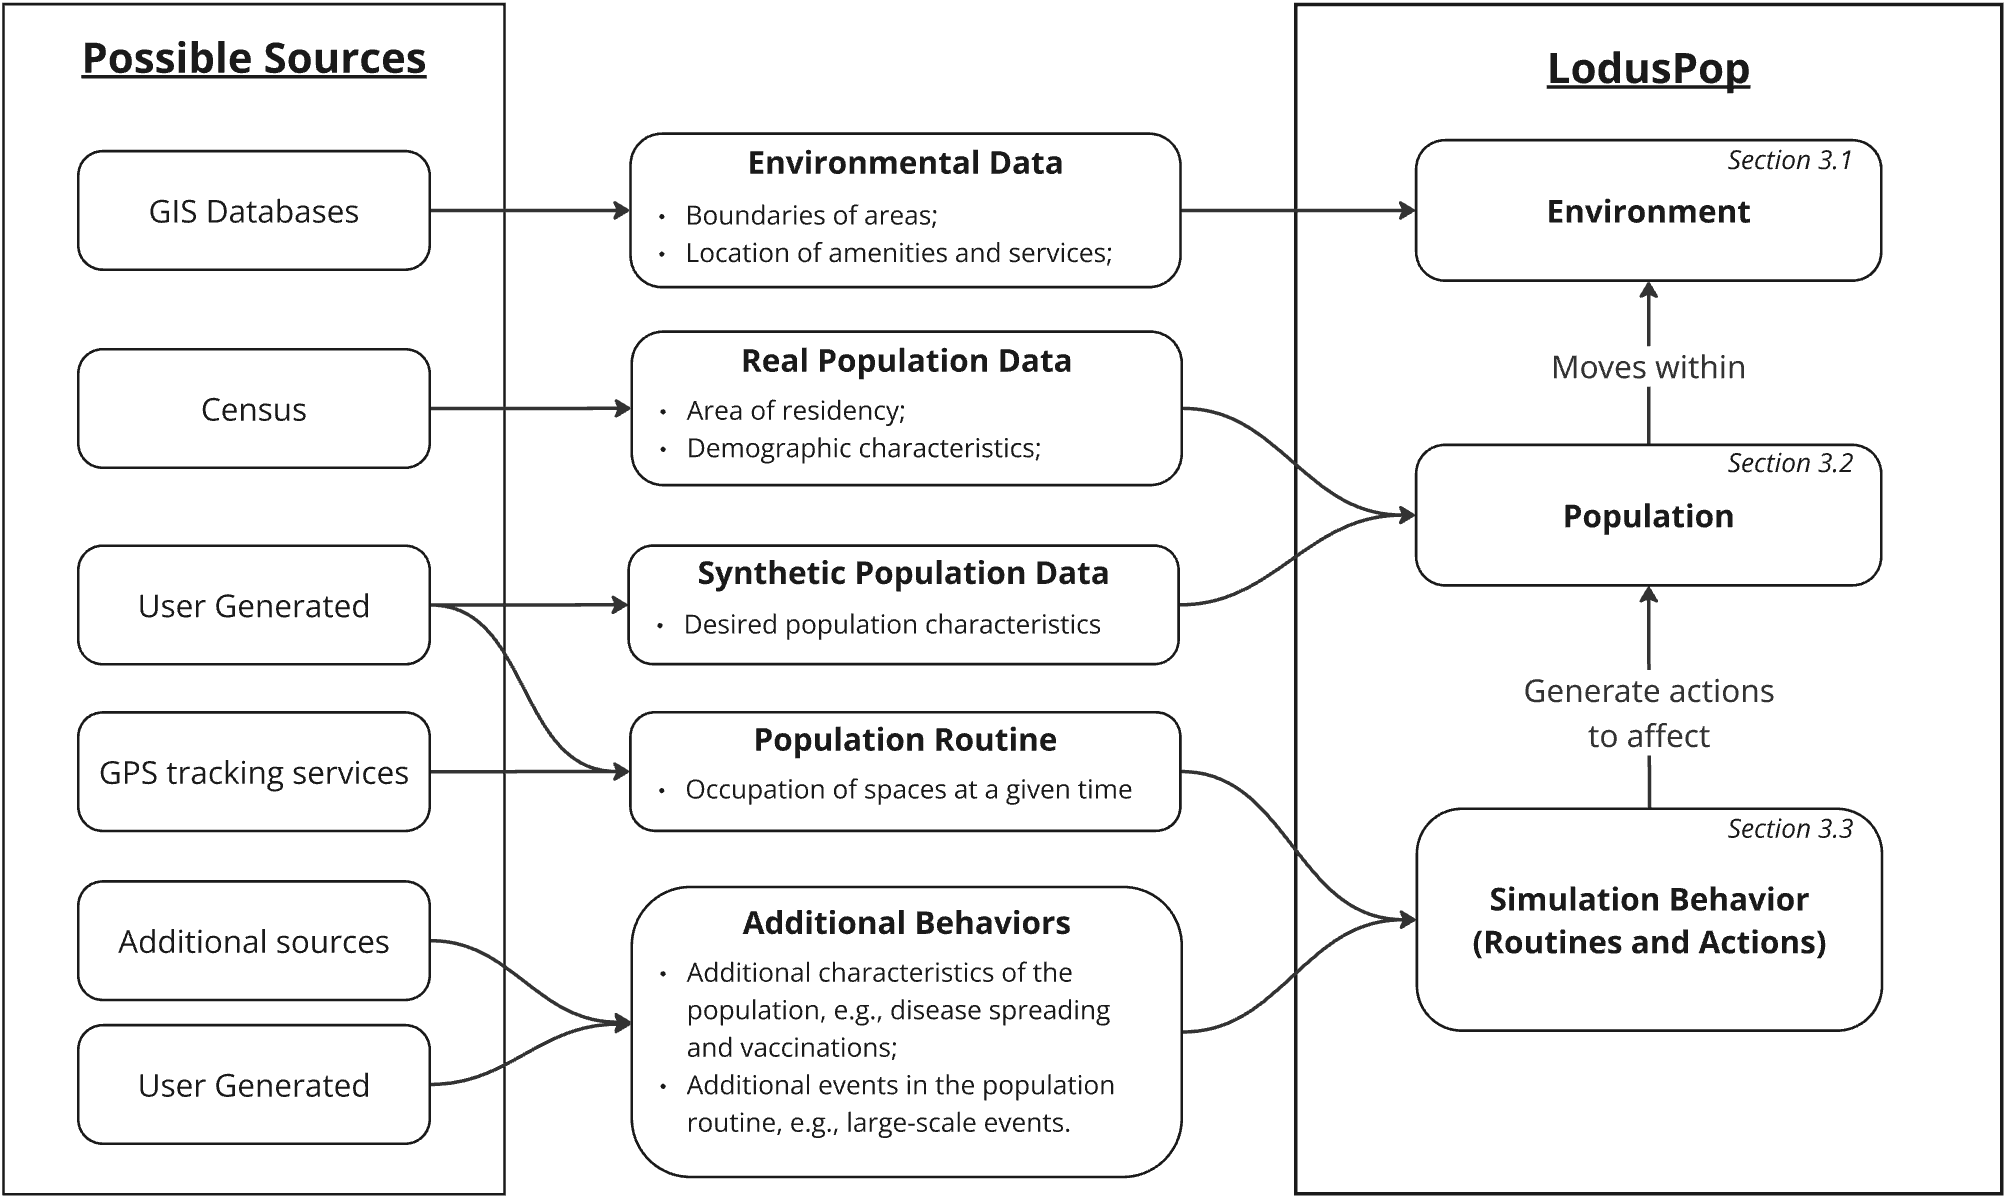
\includegraphics[width=0.98\textwidth]{Figures/DataDiagram3.png}
  \caption{\red{Flowchart illustrating the integration of data sources into the LodusPop framework. Inputs such as GIS databases, census data, user-generated data, and GPS tracking services are processed into geographic data, population characteristics, and behavioral routines. In our proposed model, routines consist of actions that influence population behavior, driving their movement through the environment. %The population and simulation behavior modules are highlighted, as they form the foundation of LodusPop and constitute the core contributions of this work.
  }
  }
  \label{fig:data_diagram}
\end{figure}

%As population mobility frameworks, in general, deal with various size scopes (e.g., neighborhoods, cities, states), we aim to bring crowd simulation strategies to human mobility simulations, in particular the capabilities of abstracting individuality in macroscopic models~\citep{thalmann2007crowd, treuille2006continuum}.
%We propose modeling the population of a simulation as blobs of people (i.e., population groups of varied sizes). In this context, Blob is an abstract structure, similar to a cloud or a legion~\citep{antonitsch2019bioclouds}, but applied to a larger population. 
%In addition, unlike BioClouds and Legion, structures formed by homogeneous populations, our blobs can contain varied individual and group characteristics, evolving in an environment with locations that can request specific population groups.

\red{Population mobility frameworks typically operate across multiple spatial scales, such as neighborhoods, cities, and states. In this work, we seek to integrate strategies from crowd simulation into human mobility modeling, particularly the ability of macroscopic models to abstract individual behaviors~\citep{thalmann2007crowd, treuille2006continuum}. To achieve this, we propose representing populations as blobs—aggregated groups of individuals of varying sizes. In this context, Blob is an abstract structure, similar to a cloud or a legion~\citep{antonitsch2019bioclouds}, but designed to represent larger and more heterogeneous populations. Unlike BioClouds and Legion, which assume homogeneous population clusters, our blobs can encompass diverse individual and group attributes and evolve within environments containing locations that demand specific population profiles.

Furthermore, our environment design builds upon the approach proposed by Silva et al.~\citep{silva2020lodus}. However, our model introduces greater flexibility, allowing regions of the simulated environment to represent different semantic entities beyond the fixed hierarchy of countries, states, regions, and cities, enabling more adaptable and context-specific representations.}

In LodusPop, we can define a set of characteristics for each blob, representing a population of a specific profile distributed in the environment and changing temporally and spatially in the simulation. For instance, one group, representing a blob, might consist of children going to school in the morning and returning home in the afternoon, illustrating spatial movement within a city. Another example involves changes in population parameters, such as healthy workers commuting to their jobs in the morning, with some individuals becoming sick during the day, resulting in healthy individuals returning home and sick individuals heading to a hospital, in this case representing a split in the blob structure.

%This paper focuses on simulating population dynamics within the LODUS environment. However, we do not present all the ideas behind the granularity of the space to provide representation in countries, states, regions, and cities (for further information, please consider~\citep{silva2020lodus}), but only data that is needed to simulate the population movement in the present work.
Our proposed model considers the following elements to provide population simulation, which will be described in the next sections. 
\begin{itemize}
    \item a) An environment modeled as a graph of regions and points of interest that the population can occupy;
    \item b) The population is modeled as blobs that can split and merge and can contain characteristics of the population; and
    \item c) a set of population movement actions and routines to describe the desired population behavior during the simulation.
\end{itemize} 



\subsection{Environment and Spatial Representation}
\label{sec:environment}

To adequate our population mobility simulation to different spatial scopes, we model the environment as an abstract graph composed of \textit{regions} and \textit{points of interest}. The regions ($R$) represent areas of physical space in the virtual world that can contain points of interest ($P$), which represent locations that motivate human travel and that can have population groups (i.e., blobs $B$). 
When setting up a simulation, users define the spatial scope that $R$ and $P$ represent. For example, in a city simulation, $R$ could correspond to districts, while $P$ might represent markets, malls, hospitals, residential buildings, and commercial centers. 


\redb{A region $R$ is represented as a set of points of interest $\{P_1, ..., P_m\}$. Each point of interest $P_i$ stores the blobs currently located there, denoted $\bm{B}_{P_i}$ and a local routine $Ro_{P_i}$
that specifies which actions occur at that location over time as the simulation evolves (\ref{sec:routines}). Table~\ref{tbl:notation_env} summarizes the notation used for regions and points of interest.} 
Additionally, Appendix~\ref{app:input} outlines the process of defining the input data necessary for designing a simulation. Appendix~\ref{app:input_environment} specifically addresses the data required to model the simulation environment.

%A region $R$ is represented as a set of $P$. In turn, $P$ represents locations that the population can occupy as they move during a simulation. A certain $P_i$ is represented by a tuple $(\bm{B}_{P_i}, Ro_{P_i})$, where $\bm{B}_{P_i}$ is a vector of zero or more population blobs currently located in $P_i$. Each $P_i$ has only one $Ro_{P_i}$, which is a local routine of actions that describes the demand for a population to be at $P_i$ over time as the simulation evolves. 

Indeed, this characterizes an inversion of responsibility compared to what usually happens in population simulations. \redb{In many agent-based approaches, populations decide where to go based on individual preferences or probabilistic rules, requiring granular data about individual movements and locations. Even in field-based models, where motion is guided by environmental potentials or vector fields, agents typically remain the entities that sample and follow these fields.
In our case, the environment is responsible for decision-making regarding the occupation of the population during the simulation, i.e., locations ask for people instead of people choosing where to go. We believe that shifting the focus to the environment as the decision-maker minimizes dependence on granular individual-level data. This shifts part of the decision logic from individuals to points of interest and regions, and is designed to minimize dependence on granular individual-level data by leveraging aggregated or generalized information about population distributions and environmental conditions. }%Instead, it leverages aggregated or generalized information about population distributions and environmental conditions to guide movement.
For example, a $P_m$ representing a market can request consumers, i.e., $P_m$ has a local routine $Ro_{P_m}$, which defines that a certain population of determined characteristics will go to the market during the simulation. $\bm{B}_{P_m}$ represents all the population blobs that are currently on the market.

Other examples in the same region $R$ can be a school that requests students, and hospitals that request patients. In these cases, school is a $P_j$ in $R$, in which $Ro_{P_j}$ is the local routine to go to the school and $\bm{B}_{P_j}$ is a specific population of students. 
\red{Similarly, the hospital is also a $P_k$ in $R$, and $Ro_{P_k}$ is a local routine that should be executed at the hospital.} 
Additionally, $\bm{B}_{P_k}$ is a particular population that goes to the hospital. \red{Figure~\ref{fig1:environment} presents a diagram of a LodusPop environment, representing regions, points of interest, and blobs.}
As humans generally tend to present cyclical behavior in their movement~\citep{gonzalez2008understanding}, repeating similar routines daily or weekly, a LodusPop simulation is also cyclical, where local routines $Ro$ repeat every time cycle of simulation. 
The user defines the temporal scope of a cycle when designing the simulation. A cycle may represent an hour, a day, a month, etc.

\begin{figure}[ht]
 \centering
  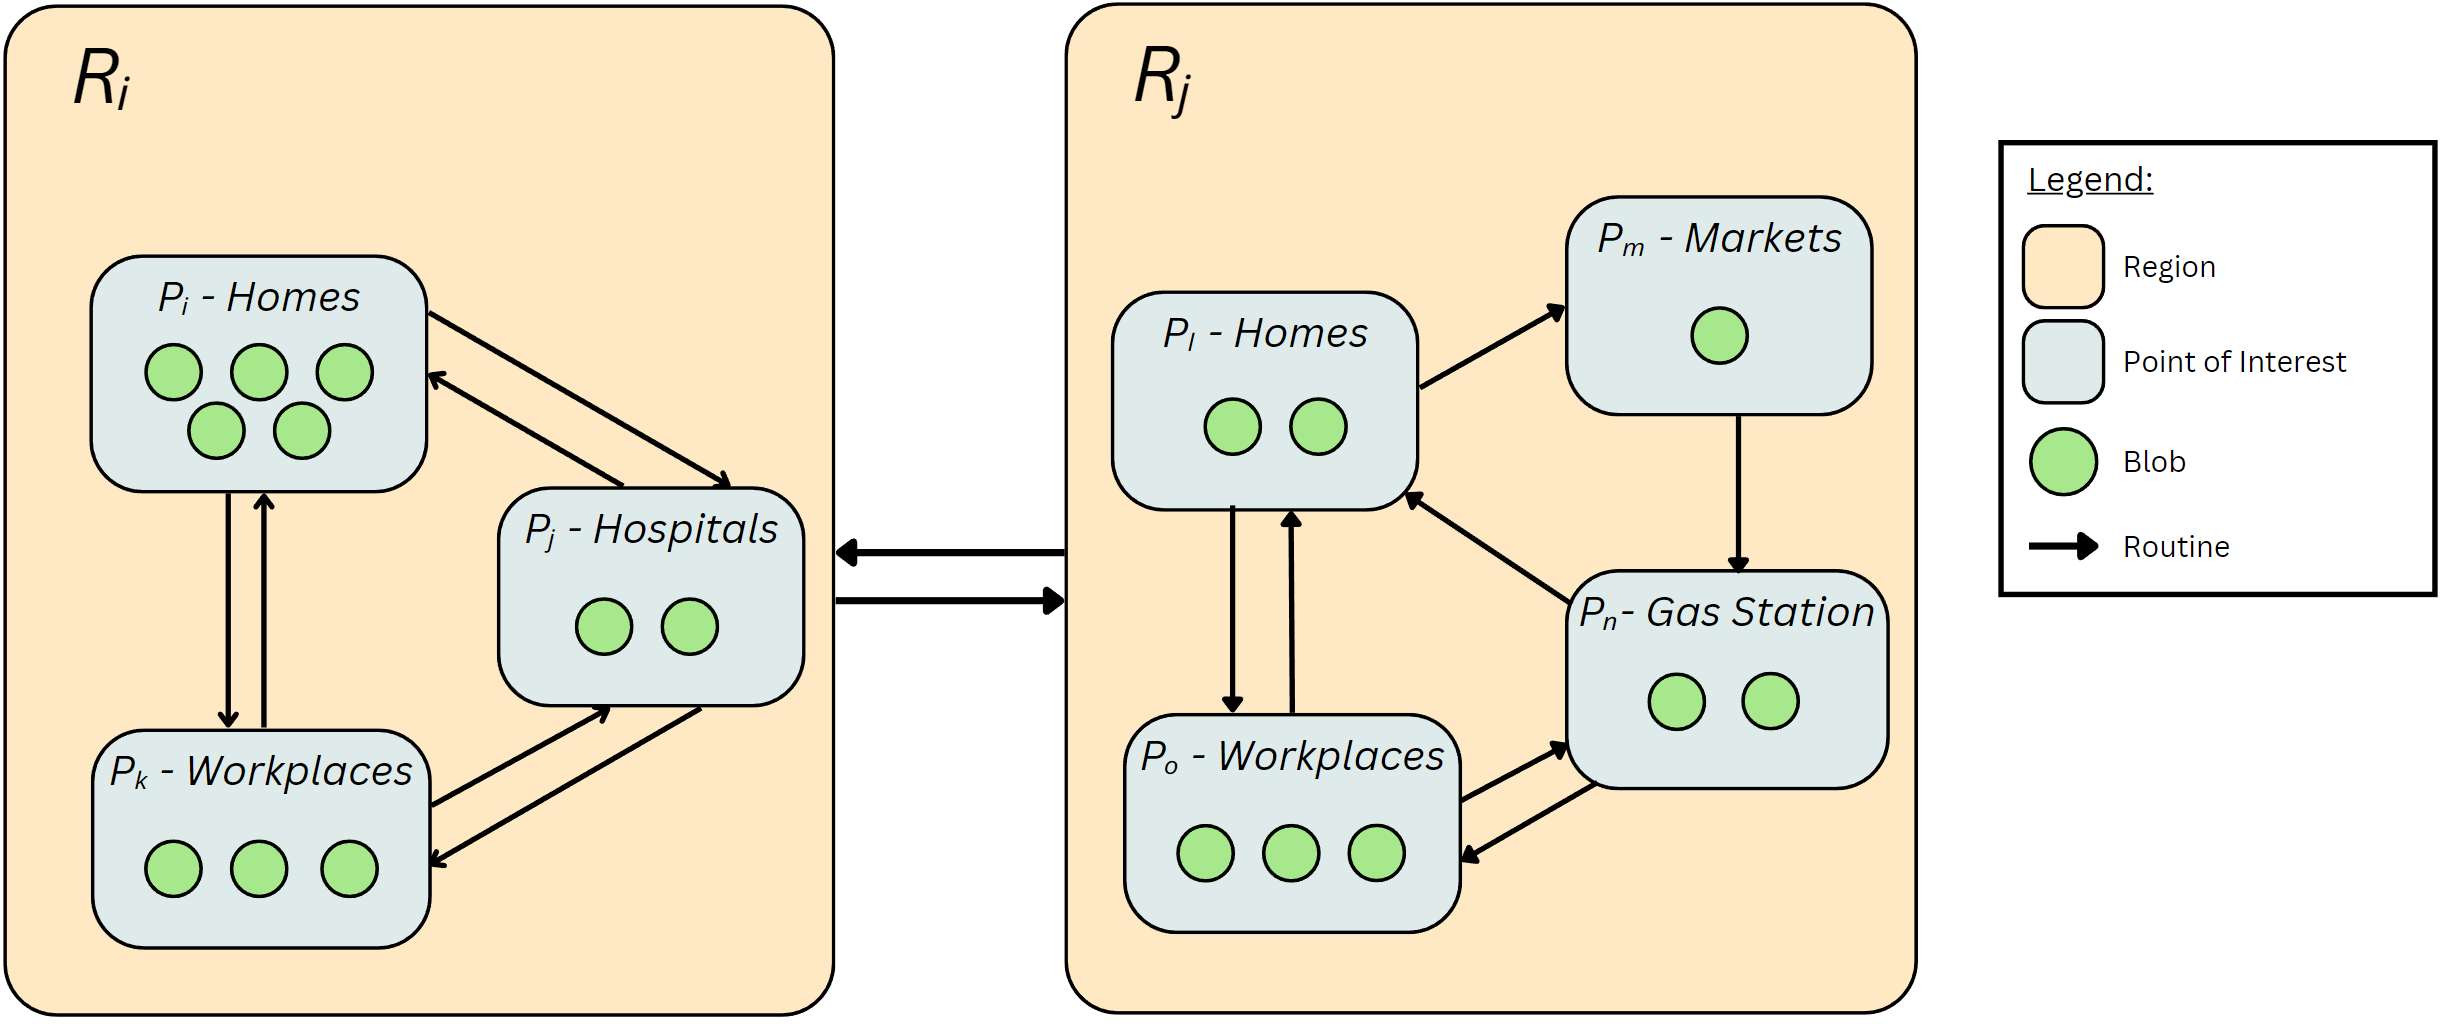
\includegraphics[width=0.98\textwidth]{Figures/Environment.png}
  \caption{\red{A diagram of a LodusPop environment. The figure presents two regions, $R_i$ and $R_j$, containing different points of interest $P$. Each point of interest may contain groups of the population (i.e., blobs), and routines are responsible for moving them in the environment during the simulation.}} 
  \label{fig1:environment}
\end{figure}



\subsection{Dynamic Availability and Dependencies}
In addition to its blobs and routine, every point of interest has a time-dependent \textit{effective availability}. Let $C_i(t)$ be the set of direct causes disabling $P_i$ at step $t$, such as an off-cycle closure or flood exposure, and let $q_i(t)=1$ exactly when $C_i(t)$ is empty. A point of interest may also declare a set $D_i^{all}$ of prerequisites that must all be enabled and one or more threshold groups $(k,G)$ requiring at least $k$ enabled prerequisites from $G$. Its effective state is
\begin{equation}
e_i(t)=q_i(t)\land
\bigwedge_{P_j\in D_i^{all}} e_j(t)\land
\bigwedge_{(k,G)\in D_i^{min}}
\left[\sum_{P_j\in G} e_j(t)\geq k\right].
\label{eq:node_availability}
\end{equation}
When no dependency rule is defined, $e_i(t)=q_i(t)$. Dependencies may be transitive, so effective states are recomputed until no state changes. Removing a cause from $C_i$ does not enable the node while another cause remains, and satisfying a direct state request does not override an unsatisfied dependency. This cause-aware formulation avoids, for example, reopening a flooded facility merely because its scheduled closure ended.

Availability records whether a location can participate in an action; it does not prescribe a universal population response. A plugin may suppress a request from a disabled origin, reject a disabled destination, retain demand in a queue, select a fallback, or reroute it. These alternatives are domain policies and are kept outside the core environment definition.



\begin{table}[h]
\redb{
\footnotesize
\centering
\caption{Mathematical notation and descriptions of the elements defined in Section~\ref{sec:environment}.}
\label{tbl:notation_env}
\begin{tabularx}{\linewidth}{@{}lcX@{}}
\toprule
\textbf{Element} & \textbf{Notation} & \multicolumn{1}{c}{\textbf{Description}} \\ \midrule
Region                                                             & $R$        & Represent areas of physical space in the virtual world that can contain points of interest. A region $R_i$ is defined as a set of $P$.  \\ \midrule
\begin{tabular}[c]{@{}l@{}}Point of\\ Interest\end{tabular}        & $P$        & Represent locations that the population can occupy as they move during a simulation. A $P_i$ is defined by a collection of population blobs ($\bm{B}_{P_i}$), its local routine ($Ro_{P_i}$), and its effective availability. \\ \midrule
\begin{tabular}[c]{@{}l@{}}Direct disable\\ causes\end{tabular}    & $C_i(t)$   & Named, independently removable causes that directly prevent $P_i$ from being available at step $t$. \\ \midrule
\begin{tabular}[c]{@{}l@{}}Dependency\\ constraints\end{tabular}  & $D_i$      & All-of and minimum-of prerequisite rules used to derive effective availability. \\ \midrule
\begin{tabular}[c]{@{}l@{}}Effective\\ availability\end{tabular} & $e_i(t)$   & Boolean state obtained from the direct causes and the effective states of all prerequisites. \\  \bottomrule
\end{tabularx}
} %end of \redb
\end{table}




\subsection{Population Representation}
\label{sec:population}
%The population in LodusPop is represented by the abstraction of people as already defined blobs $B$, always located in some point of interest.
The population in LodusPop is represented by an abstraction of people into blobs $B$, each always located at some point of interest. These blobs describe the population in groups rather than tracking individuals.
\redb{
%A blob represents a group of individuals that share the same traceable and sampled characteristics at a given point of interest. 
Formally, we denote a blob as $B = (TP, \bm{Tc}, \bm{Sc})$ where $TP$ is the total number of individuals in the blob, $\bm{Tc}$ is the collection of traceable characteristics, and $\bm{Sc})$ is the collection of sampled characteristics. Table~\ref{tbl:notation_pop} summarizes this notation and the associated terminology.

We distinguish two types of characteristics. \textit{Sampled Characteristics}, collected in $\bm{S_c}$, are attributes represented by their distribution within the blob. For example, a sampled characteristic \textit{Age} may have categories \textit{Child}, \textit{Adult} and \textit{Elder}, each associated with a certain number of individuals. By combining multiple sampled characteristics, we can jointly describe attributes such as age, level of schooling and employment status.
\textit{Traceable Characteristics}, collected in $\bm{T_c}$, are attributes whose values are explicitly stored as a single value for the entire blob, rather than as a distribution over categories. For instance, a traceable characteristic \textit{Vaccination status} with values \textit{Vaccinated} and \textit{Unvaccinated} implies that each blob in the simulation is composed entirely of vaccinated or entirely of unvaccinated individuals.
}

These characteristics allow us to specify the population in more detail, e.g., elderly people who are currently vaccinated against a given disease or the number of adults who commute to work by bus. Following the previous examples, it becomes possible to track vaccination by age group in the simulation by identifying all blobs $B$ with a \textit{Vaccinated} status and their respective \textit{Age} distributions. Figure~\ref{fig2:blob_diagram} shows a diagram of a blob, including its characteristics and associated distributions. Appendix~\ref{app:input_population} presents an example of the input data required to model the initial population in simulations.

%A blob $B$ is represented as a set of attributes that describe the population to be simulated. For example, an attribute representing the characteristic \textit{Age} may have \textit{Child}, \textit{Adult}, and \textit{Elder} as possible categories (or values), each associated with a certain number of people. Using a collection of attributes, the population can be modeled with multiple characteristics, such as age, level of schooling, and employment status. These attributes are referred to as \textit{Sampled Characteristics}, and all blobs $B$ must have at least one of them.
%Blobs can also have a second set of characteristics, named \textit{Traceable Characteristics}, modeled as pairs of values instead of categories. For example, we can model a \textit{Vaccination Status} characteristic with the possible values: \textit{Vaccinated} and \textit{Unvaccinated}, so each blob in the simulation will be composed of people who are either all vaccinated or all unvaccinated. Sampled and traceable characteristics can be created to specify better a population, e.g., elderly people who are currently vaccinated against a given disease or the number of adults who go to work by bus. 
%Following the previous examples, it becomes possible to track vaccination per age group in the simulation by identifying all blobs $B$ with a \textit{Vaccinated} status and their respective \textit{Age} distribution. \redb{Table~\ref{tbl:notation_pop} lists the mathematical notation and descriptions of the elements introduced in this section.}




%Detailing the blob $B_i$, it is defined as a tuple $(TP_i, \bm{Tc}_i, \bm{Sc}_i)$, where $TP_i$ is the total population size (scalar value), $\bm{Tc}_i$ is a vector of traceable characteristics (pairs of values), and $\bm{Sc}_i$ is a vector of sampled characteristics.
%Each traceable characteristic $j$ in $\bm{Tc}_i$ is composed of an identifier (i.e., a string) and its value (not restricted by type).
%Each sampled characteristic $k$ in $\bm{Sc}_i$ is also a tuple $(N_k, \bm{D}_k)$, where $N_k$ is the string identifier of this characteristic (e.g., age or occupation), and $\bm{D}_k$ is the vector that contains the categories of the population in that given characteristic. 
%A sample characteristic may contain any number of labeled scalar values, e.g., \textit{age} represented as the labels \textit{children}, \textit{adults} and \textit{elders}, having respectively 20, 40, and 10 individuals. The sum of populations at each distribution in $\bm{Sc}_i$ must equal the total population $TP_i$ which is part of blob definition. 
%Figure~\ref{fig2:blob_diagram} contains a diagram of a blob, representing its characteristics, and containing distributions.
%Appendix~\ref{app:input_population} presents an example of the input data required to model the initial population in simulations.


As mentioned before, during the simulation, blobs in $P_i$ are affected by the local routine $Ro_{P_i}$.
Routines can select a specific population profile to be affected, e.g., moving only children to school, i.e., people from a particular sample attribute ``Age'' in the category ``child'' should go from $P_i$ to $P_j$.
This type of operation in the population $B_i$ of a certain $P$ uses a population template. 

\redb{A population template $T$ specifies which individuals are affected by an action and in what quantity. We represent it as $T = (T_Q, \bm{T_{Tc}}, \bm{T_{Sc}})$, which specifies i) the quantity of people to be affected, ii) an optional a set of predicates on traceable characteristics, and iii) is an optional set of predicates and distributions on sampled characteristics. When applied to a set of blobs, a template behaves as a filter that identifies the subset of individuals that satisfy all predicates and are counted towards $T_Q$.}
%where $T_Q$ is the quantity of people to be affected (for example, an absolute number or a fraction of the eligible population), 
%$\bm{T_{Tc}}$ is an optional a set of predicates on traceable characteristics, and  $\bm{T_{Sc}}$ is an optional set of predicates and distributions on sampled characteristics. When applied to a set of blobs, a template behaves as a filter that identifies the subset of individuals that satisfy all predicates and are counted towards $T_Q$. }
%A blob $B_i$ is only affected by the template $T$ if its traceable or sampled properties are specified in $T$. Indeed, $T$ operates as a filter to select a population from $B$.

\begin{figure}[ht]
 \centering
  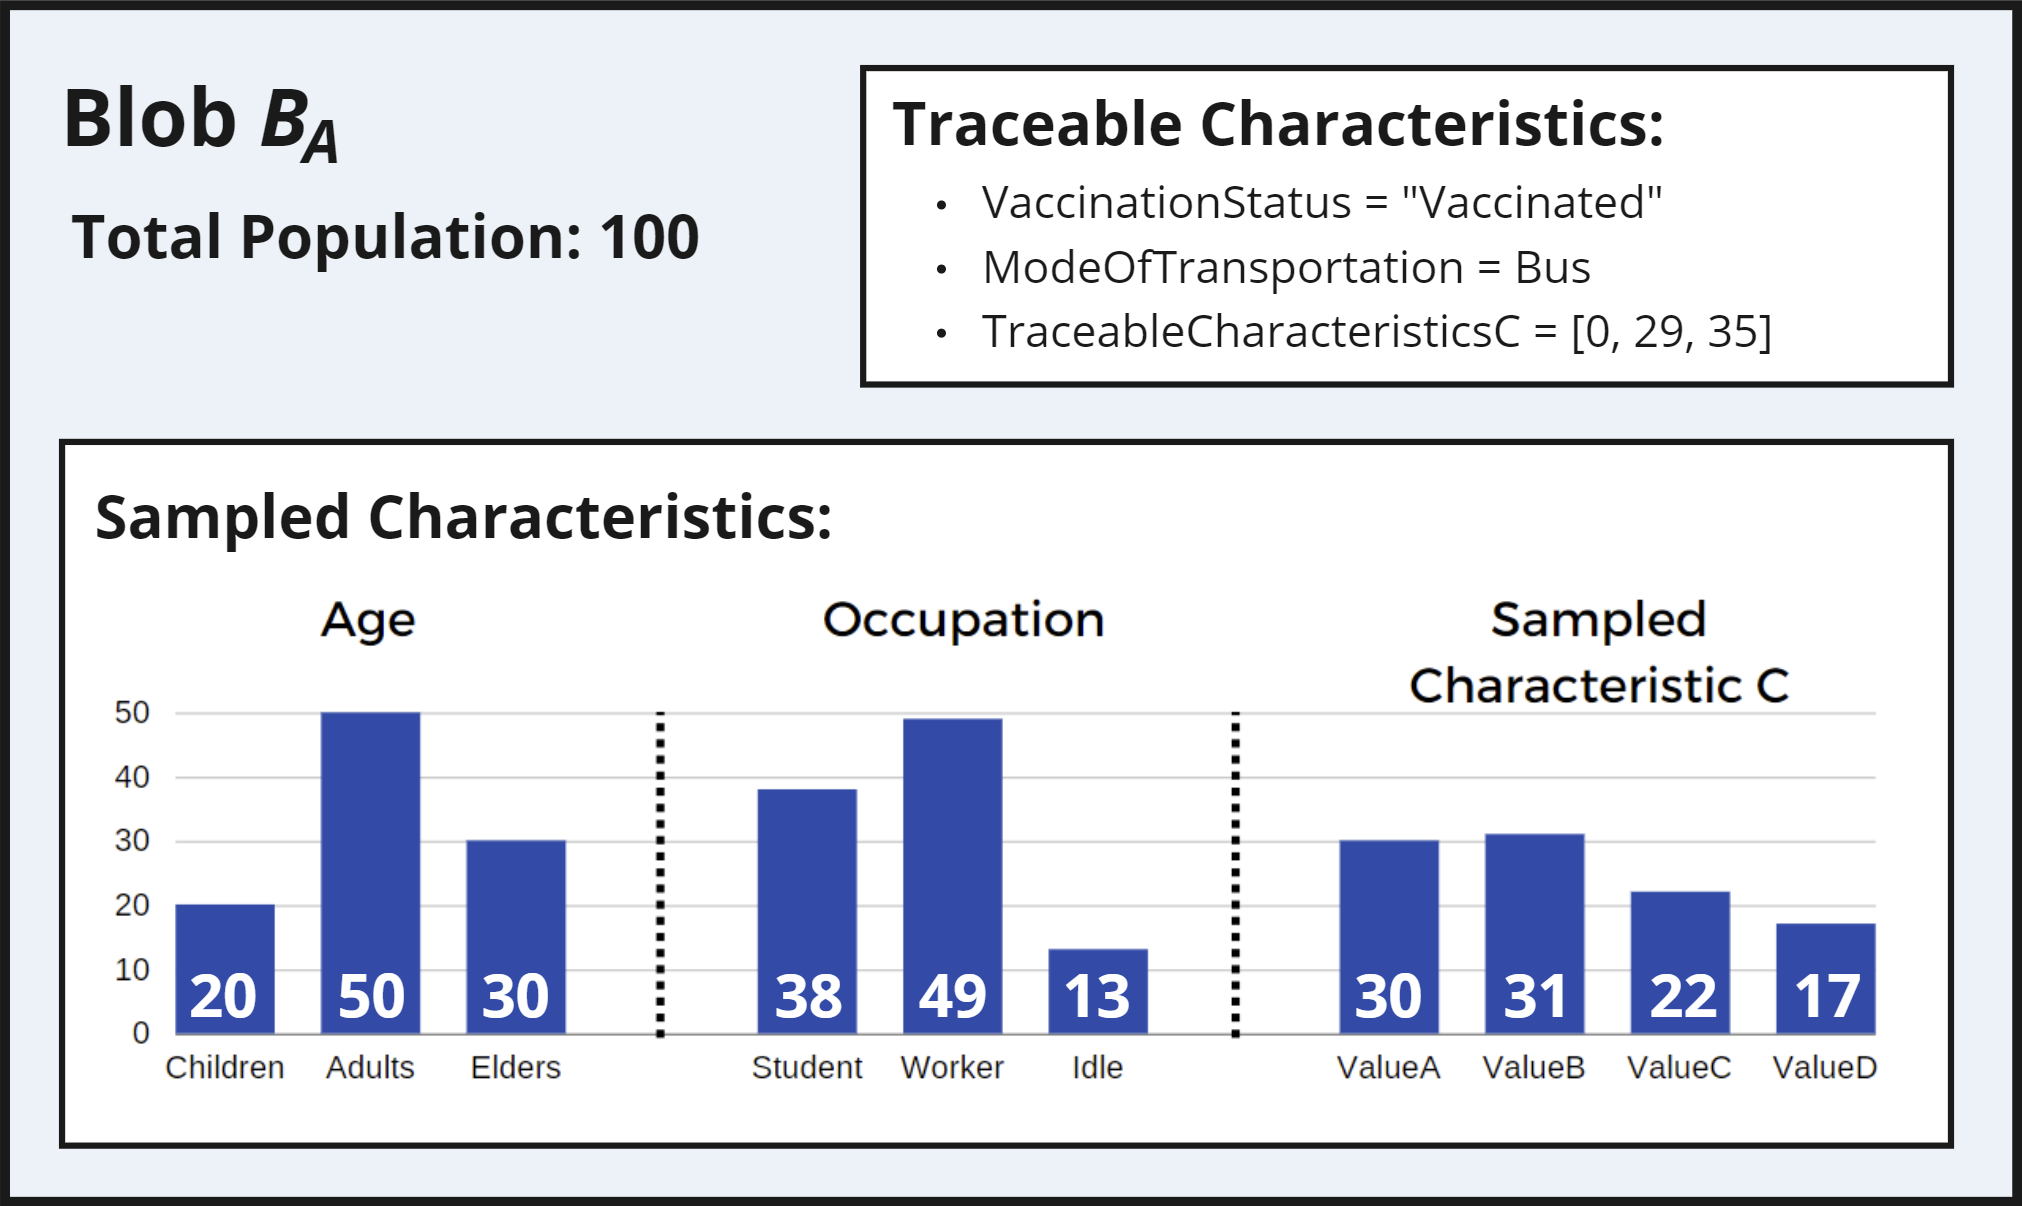
\includegraphics[width=0.9\textwidth]{Figures/BlobDiagram.png}
  \caption{Diagram of a Blob $B_A$ containing 100 people, three traceable characteristics, and three sampled characteristics. Traceable characteristics describe the entire blob population and can have any value type. The distribution of each sampled characteristic sum should be equal to the total population of the blob.} 
  \label{fig2:blob_diagram}
\end{figure}

Consider a blob $B_j$ with two sampled characteristics: \textit{i)} \textit{Age}, which includes the possible values \textit{Children}, \textit{Adults}, and \textit{Elders}, and \textit{ii)} \textit{Occupation}, with possible values \textit{Student} and \textit{Worker}. A template $T$ that specifies \textit{Age=Adults} in its collection of sampled characteristics will target only the specified group within $B_j$, in this case, only adults. If the template $T$ does not include a filter for the second sampled characteristic (Occupation), all occupation categories in $B_j$ are affected. The number of affected individuals in categories such as Students and Workers is determined proportionally based on their distribution within $B_j$. For instance, if $B_j$  contains more students than workers, a larger proportion of students will be selected. This process continues until the total number of individuals defined in $T$ is selected or until there are no remaining eligible individuals in $B_j$.

% Splits
When a blob is operated using a population template $T$, it is possible that only a portion of its population may be affected, e.g., a blob $B_i$ that has 75 people and only 20 are selected in $T$. If the operation is to move to another $P$, then such 20 people will create a new blob. This operation generates a split, i.e., the original blob will be separated into two smaller ones. 
In such an example, a template with quantity $T_Q = 20$ selects 20 people from $B_i$ and splits it by creating a new blob $B_j$, which is moved to a different $P$. 
The same occurs when modifying a blob's $\bm{Tc}$s. For example, another blob $B_k$ has 90 \textit{Healthy} people, 
and 20 are selected, using $T$, to be infected by a disease. The split occurs, and a \textit{InfectionStatus} of $B_l$ (newly created blob) is changed to \textit{Infected}.

% Merge
In addition to split operations, blobs can also be merged, combining their total populations $TP$. 
Each sampled characteristic of the resulting blob is the sum of the respective characteristics of the merged blobs. A merge can only occur between blobs currently in the same $P$ and with the same values in all their traceable characteristics. This restraint allows us to merge only populations that share the same traceable features.
% Figure
Figure~\ref{fig3:blob_operations_with_template} presents a diagram of blobs affected by two templates, resulting in splits and merges. The first scenario, depicted at the top of the figure, demonstrates the relocation of a population. %In 1a), the initial blob $B_i$ has a population of 100 located in $P_i$. In 1b), a template $T$ selects 30 individuals, resulting in the split of $B_i$ and the creation of $B_j$. In 1c), $B_j$ is transferred to $P_j$. 
The second scenario illustrates changes in traceable characteristics of a population.% In 2a), two blobs, $B_i$ containing 100 unvaccinated individuals (depicted in red) and $B_j$ containing 50 vaccinated individuals (depicted in green), coexist in $P_i$. In 2b), a template $T$ selects 20 unvaccinated individuals, affecting only $B_i$ and creating $B_k$. In 2c), the traceable characteristic "VaccStatus" of $B_k$ is modified to "Vaccinated." In 2d, $B_k$ is merged with $B_j$ as they now share the same characteristics and exist within the same $P_i$.

\begin{figure}[ht]
 \centering
  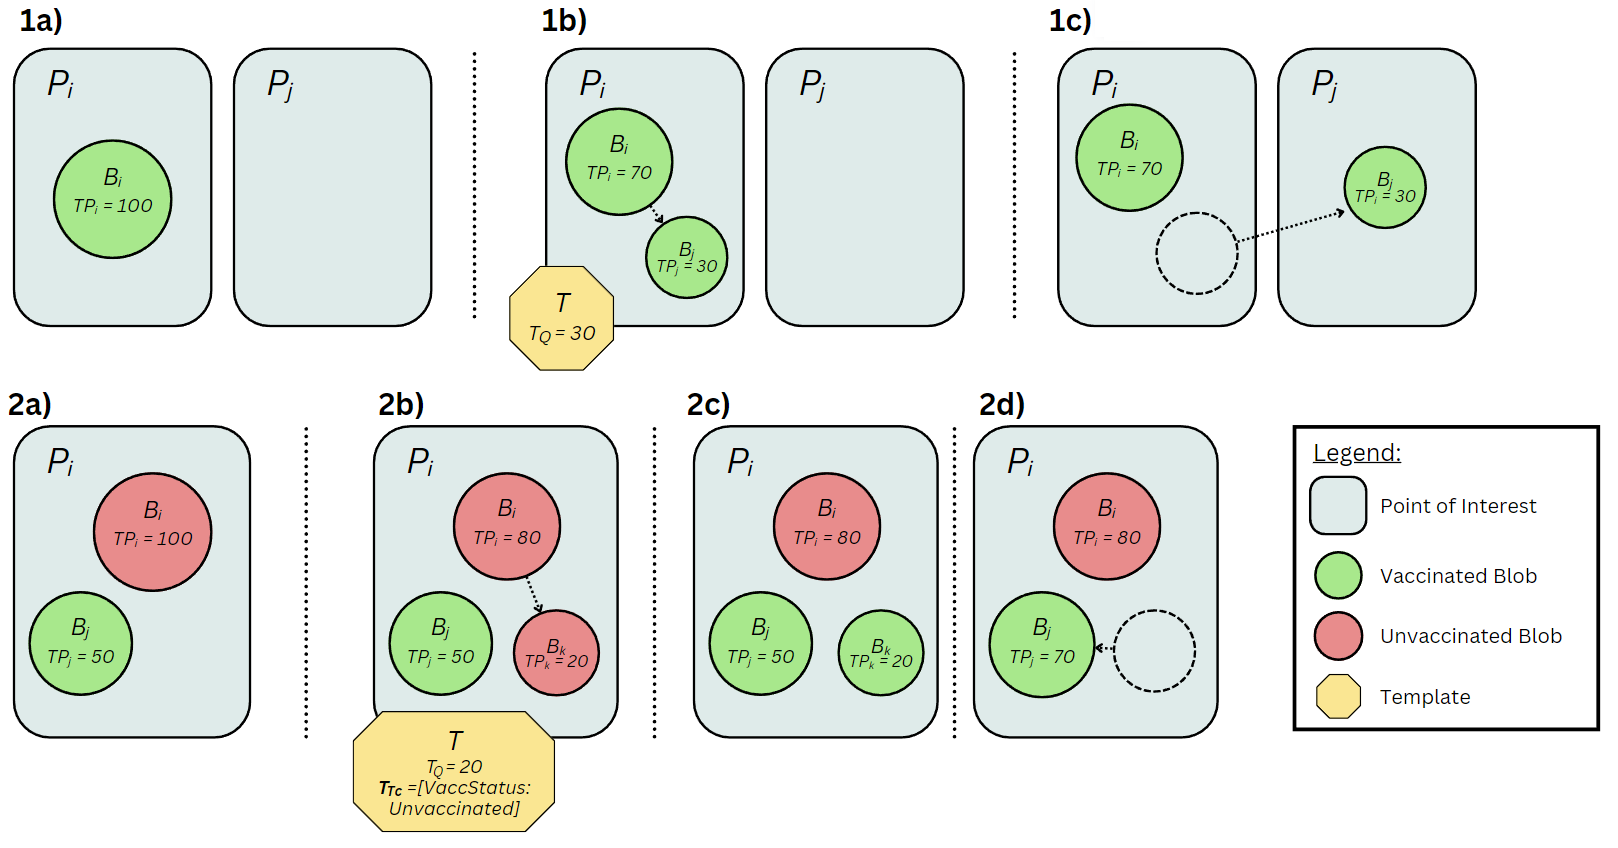
\includegraphics[width=0.99\textwidth]{Figures/BlobOperations.png}
  \caption{
  Diagram presenting two scenarios of blobs being modified. The first scenario (1) (on the top) shows a population being moved to another location. In 1a, the initial blob $B_i$ has a population of 100. In 1b, a template $T$ selects 30 people, splitting $B_i$ and creating $B_j$. In 1c, $B_j$ is moved to $P_j$. The second scenario (2) shows a population's traceable characteristics changed. In 2a, there are two blobs, $B_i$ containing 100 unvaccinated people (in red), and $B_j$ containing 50 vaccinated people (in green). In 2b, a template $T$ selects 20 unvaccinated people, affecting only $B_i$ and splitting it into $B_k$. In 2c, the traceable characteristic \textit{VaccStatus} of $B_k$ is changed to \textit{Vaccinated}. In 2d, $B_k$ is merged into $B_j$ since they now share the same characteristics and are in the same $P_i$.
  } 
  \label{fig3:blob_operations_with_template}
\end{figure}

\begin{table}[h]
\redb{
\footnotesize
\centering
\caption{Mathematical notation and descriptions of the elements defined in Section~\ref{sec:population}.}
\label{tbl:notation_pop}
\begin{tabularx}{\linewidth}{@{}lcX@{}}
\toprule
\textbf{Element}                                                             & \textbf{Notation} & \multicolumn{1}{c}{\textbf{Description}}                                                                                                                                                                                                                                                                                     \\ \midrule
Blob                                                               & $B$        & Represent an abstraction of the population. A $B_i$ is defined as its total population ($TP_i$), a collection of traceable characteristics ($\bm{Tc}_i$), and a collection of sampled characteristics ($\bm{Sc}_i$)                                                                                                         \\ \midrule
\begin{tabular}[c]{@{}l@{}}Traceable\\ Characteristic\end{tabular} & $Tc$       & Characteristic of a blob defined as an identifier (i.e., a string) and its value (not restricted by type).                                                                                                                                                                    \\ \midrule
\begin{tabular}[c]{@{}l@{}}Sampled\\ Characteristic\end{tabular}   & $Sc$       & Characteristic with a categorical distribution over the blob population. Defined as a string identifier and a collection of its possible categories, each associated with a certain number of people.                                                                                                                             \\ \midrule
\begin{tabular}[c]{@{}l@{}}Population\\ Template\end{tabular}      & $T$        & Specifies which individuals are affected by an action and in what quantity, operating as a filter to select a population from a $B$.                 \\ \bottomrule
\end{tabularx}
} %end of \redb
\end{table}



\subsection{Actions, Routines, and Simulation Time}
\label{sec:routines}

\redb{All behavioral dynamics in LodusPop are driven by routines, which associate discrete time steps with actions that operate on blobs.
We consider a simulation organized into cycles of fixed length 
$d$ steps. Within a cycle, time is indexed by an integer $t \in \{0, ..., d-1\}$, which we refer to as the cycle step. 

A (local or global) routine is a finite set of pairs $R = \{(t, A)\}$, where $t$ is a cycle step and $A$ is an action to be executed at that step.
For each point of interest $Pi$, the local routine is denoted $Ro_i$ and specifies the actions that should be performed by $Pi$.
The Global Routine $GRo$ has the same structure but applies its actions to all points of interest in the environment.

Each action $A$ is defined as $A = (N, T, \bm{V})$, where $N$ is an identifier for the action type (e.g., MOV or CH); $T$ is a population template as defined in Section~\ref{sec:population}, selecting the subset of a blob that will be affected; and $\bm{V}$ is a vector of additional values (parameters) used by the action. 
Table ~\ref{tbl:notation_rout} summarizes the notation introduced in this section.

In the core implementation, LodusPop provides two built-in action types:
\textit{move population} (MOV), which moves a subset of a blob between points of interest; and \textit{change traceable characteristic} (CH), which modifies the traceable characteristics of a subset of a blob.

A MOV action expects its parameter vector $\bm{V}$ to specify an origin and a destination point of interest. For example, the local routine of $P_i$ may include the pair $(t = 15, A)$, where $A = (MOV, T_i, V_i)$, with $T_i=(T_Q=20, T_{Tc}=\emptyset, T_{Sc}=\{Age=Child\})$, and $V_i$ encoding $P_i$ as origin and $P_j$ as destination. At cycle step $t = 15$, this action selects 20 children from the blobs at $P_i$ , splits them into a new blob, and moves that blob to 
$P_j$.

A CH action expects $\bm{V}$ to contain the name of a traceable characteristic and its new value. For instance, the local routine of $P_j$ may include $(t = 25, A')$, with $A' = (CH, T_j, V_j)$, where $T_i=(T_Q=20, T_{Tc}=\{Status=Unvaccinated\}, T_{Sc}=\emptyset)$, and $\bm{V_j}$ encodes the update ``Status := Vaccinated''. At cycle step $t=25$, this action selects 20 unvaccinated individuals from the blobs at $P_j$, splits them into a new blob, and changes the traceable characteristic Status of that blob to Vaccinated. Figure~\ref{fig3:blob_operations_with_template} illustrates both the movement and characteristic-change scenarios.

}

%Routines model the repeating temporal behavior of population $B$ located in any given $P$. The local routine of $P_i$ is defined as $Ro_{P_i}\xrightarrow{}\{t,A_i\}^\ast$, where $t$ is the time in the simulation that action $A_i$ should be performed. A given action $A_i$ is defined as a tuple $(N_{i}, T_{i}, \bm{V}_{i})$, where $N_{i}$ is an identifier for the action type, $T_{i}$ is a population template describing the profile and quantity of people being affected (as described in the last section), and $\bm{V}_{i}$ is a collection of values that can be used in action.

%LodusPop contains two types of actions: \textit{move population} (MOV), and \textit{change traceable characteristic} (CH).
%The \textit{move population} action type is responsible for moving a group of people in the environment and must receive the origin and destination of the movement, i.e., $P_i$ and $P_j$, respectively.
%For example: $Ro_{P_i}=\{15, \{MOV, T_i=\{20, \{\},\{age=child\}\}, P_j\}\}$, i.e., at time 15 of the simulation, 20 people from $B_i$ located at $P_i$ will move to $P_j$.
%The \textit{change traceable characteristic} action type is responsible for modifying the $\bm{Tc}$s of blobs. It must receive the identifier of the traceable characteristic being changed and its new value. One example is following described:  $Ro_{P_j}=\{25, \{CH, T_j=\{20,\{status=unvaccinated\}, \{\}\}, status=vaccinated\}\}$, i.e., at time 25 of simulation, 20 people from $B_j$ located at $P_j$ will change this status of vaccination. Figure~\ref{fig3:blob_operations_with_template} presents a diagram of blobs affected by the two detailed actions. The first scenario represents a \textit{move population} action, where a blob is moved from $P_i$ to $P_j$, and the second scenario presents a \textit{change traceable characteristic} action.

% Global routines and Queueing
The same action representation is used by the Global Routine $GRo$. For example, a MOV or CH entry in $GRo$ is executed at the specified cycle step 
$t$ for all points of interest simultaneously, enabling the modeling of global phenomena such as random walks or disease spread. Appendix~\ref{app:input_routine} provides an example of the input data used to encode both local routines and the Global Routine.

%LodusPop is also an additional resource for modeling the global behavior of a simulation.The Global Routine can be used to model global events, e.g., random walks and the spread of diseases.The Global Routine is defined as $GRo\xrightarrow{}\{t,A\}^\ast$, where $t$ is the time in the simulation that action $A$ is performed by all $P$s in the environment. Appendix~\ref{app:input_routine} presents an example of the input data required to model a Global Routine ($GRo$) and the local routines for specific points of interest.

% New action types with Plugins
%New action types can be included in the simulator using plugins. A plugin can add another action type and a function to consume it. Actions included by plugins have the exact definition as previously described. Considering a new action $A_j$, the system is responsible for matching the identifier for the action type $N_{A_j}$ with the function that should consume it, sending the population template $T_{j}$ and additional values $\bm{V}_{j}$ as parameters the function. Appendix~\ref{app:plugin} provides an example of how plugins can be used to introduce new action types into simulations.

To achieve repeating temporal behavior, the simulation iterates over cycle steps $t = 0, ..., d-1$ within each cycle. At the beginning of each step 
$t$, the simulator collects all actions $(t,A)$ from $GRo$ and from every local routine. For each action, it:
\begin{enumerate}
    \item uses the template $T$ to select the affected population from the current blobs;
    \item applies the action semantics (e.g., move or characteristic change), which may split existing blobs or create new ones; and
    \item performs, at the end of the step, a merge operation at each point of interest, combining blobs that share identical traceable characteristics.
\end{enumerate}

Figure~\ref{fig:simulation_diagram} illustrates the simulation behavior over a single cycle. Appendix~\ref{app:simulator} presents an example of a simulation script that manages the overall control of the simulation flow. \redb{In the current implementation, actions scheduled for the same cycle step are executed sequentially in the order in which they are listed in the input, and we apply the same ordering to actions in the global routine $GRo$. 
Each action is treated as an atomic operation: it selects a population according to its template based on the current blob configuration, applies the corresponding modifications, and immediately updates the state before the next action is evaluated. As a consequence, the same blob (or its descendants) may be affected by multiple actions within a single cycle step, but the later actions always see the state resulting from earlier ones in that step.}


%To achieve a repeating temporal behavior for $P$s, the simulation execution comprises cycles that repeat every $d$ step, with each step named a \textit{cycle step}.
%The simulation designer can define the temporal scope of a simulation by specifying the semantics of a cycle step and the total cycle duration $d$. For instance, a cycle with $d = 24$ could represent a 24-hour day, where each cycle step corresponds to one hour, or a two-year period, where each step represents a month.
%For a given point of interest $P_k$, all actions in its local routine $Ro_{P_k} \xrightarrow{}\{t,A\}^\ast$ are executed once per cycle, where $t$ denotes the cycle step at which an action $A$ is performed. The same principle applies to the global routine $GRo$.
%Appendix~\ref{app:simulator} presents an example of a simulation script that manages the overall control of the simulation flow.

%Figure~\ref{fig:simulation_diagram} illustrates the simulation behavior process. \redb{In the current implementation, actions scheduled for the same cycle step are executed sequentially. For each point of interest $P_k$, we process all actions in its local routine $Ro_{P_k}$ in the order in which they are listed in the input, and we apply the same ordering to actions in the global routine $GRo$. 
%Each action is treated as an atomic operation: it selects a population according to its template $T$ based on the current blob configuration, applies the corresponding move or characteristic change (possibly splitting blobs), and immediately updates the state before the next action is evaluated.
%As a consequence, the same blob (or its descendants) may be affected by multiple actions within a single cycle step, but the later actions always see the state resulting from earlier ones in that step. After all actions at a given cycle step have been processed,} each point of interest examines its blobs in $\bm{B}_{P}$ for potential merging, combining blobs that share identical values for all traceable characteristics.


%Figure~\ref{fig:simulation_diagram} illustrates the simulation behavior process. At the start of each cycle step $t$, all actions scheduled for execution at that step are identified from the Global Routine ($GRo$) and the Local Routines of each $P$. For each action, the affected population is selected based on their template. Subsequently, each blob is modified according to the action type. These updates may result in the blob splitting, such as moving a subset of the population to a new point of interest or altering the characteristics of a portion of the blob (as shown in Figure~\ref{fig3:blob_operations_with_template}). Finally, each point of interest examines its blobs in $\bm{B}_{P}$ for potential merging, combining blobs that share identical values for all traceable characteristics.


\begin{figure}[ht]
 \centering
  
\includegraphics[width=0.99\textwidth]{Figures/SimulationBehaviorDiagram.png}
  \caption{Diagram of the simulation behavior, illustrating the identification and execution of actions from global and local routines. 
  \redb{At each cycle step, all actions scheduled for that step are collected and executed sequentially in the order defined by the simulation input. Each action modifies blobs by moving them or changing their traceable characteristics and may cause splits; subsequent actions in the same step operate on this updated state.} At the end of the step, blobs with identical traceable characteristics in the same point of interest are merged.} 
  \label{fig:simulation_diagram}
\end{figure}



\begin{table}[h]
\redb{
\footnotesize
\centering
\caption{Mathematical notation and descriptions of the elements defined in Section~\ref{sec:routines}.}
\label{tbl:notation_rout}
\begin{tabularx}{\linewidth}{@{}lcX@{}}
\toprule
\textbf{Element}                                                             & \textbf{Notation} & \multicolumn{1}{c}{\textbf{Description}} \\ \midrule
\begin{tabular}[c]{@{}l@{}}Local\\ Routine\end{tabular}            & $Ro$       & Model the repeating temporal behavior of a population $B$ located in any given $P$. It is defined as $\{t,A_i\}^\ast$, where $t$ is the time in the simulation that action $A_i$ should be performed.                                                                                                               \\ \midrule
\begin{tabular}[c]{@{}l@{}}Global\\ Routine\end{tabular}           & $GRo$      & Modeling the global behavior of a simulation. Similar to a Local Routine, but it is applied to all $P$s in the simulation                                                                                                                                                                                           \\ \midrule
Action                                                             & $A$        & Represents an action to be performed in the population, either moving or changing its characteristics. A $A_i$ is defined as an identifier for the action type ($(N_{i}$), a population template to select the population to be affected ($T_{i}$), and a collection of values to be used by the action ($\bm{V}_{i})$. \\ \bottomrule
\end{tabularx}
} %end of \redb
\end{table}

% Tabela completa
%Table~\ref{tbl:notation} provides an overview of the mathematical notation and descriptions for elements presented in this section, e.g., a region ($R$) and a point of interest ($P$). The table serves as a reference for the key elements and their definitions.

\begin{comment}
    

\begin{table}[h]
\redb{
\footnotesize
\centering
\caption{Mathematical notation and descriptions of the elements defined in Section~\ref{sec:proposed_model}.}
\label{tbl:notation}
\begin{tabularx}{\linewidth}{@{}lcX@{}}
\toprule
\textbf{Element}                                                             & \textbf{Notation} & \multicolumn{1}{c}{\textbf{Description}}                                                                                                                                                                                                                                                                                     \\ \midrule
Region                                                             & $R$        & Represent areas of physical space in the virtual world that can contain points of interest. A region $R_i$ is defined as a set of $P$.                                                                                                                                                                              \\ \midrule
\begin{tabular}[c]{@{}l@{}}Point of\\ Interest\end{tabular}        & $P$        & Represent locations that the population can occupy as they move during a simulation. A $P_i$ is defined by a vector of population blobs ($\bm{B}_{P_i}$) and its local routine ($Ro_{P_i}$)                                                                                                                         \\ \midrule
Blob                                                               & $B$        & Represent an abstraction of the population. A $B_i$ is defined as its total population ($TP_i$), a vector of traceable characteristics ($\bm{Tc}_i$), and a vector of sampled characteristics ($\bm{Sc}_i$)                                                                                                         \\ \midrule
\begin{tabular}[c]{@{}l@{}}Traceable\\ Characteristic\end{tabular} & $Tc$       & Represents a characteristic of the population in a blob. It is defined as an identifier (i.e., a string) and its value (not restricted by type).                                                                                                                                                                    \\ \midrule
\begin{tabular}[c]{@{}l@{}}Sampled\\ Characteristic\end{tabular}   & $Sc$       & Represents a characteristic of the population in a blob. It is defined as a string identifier and a vector of its possible categories, each associated with a certain number of people.                                                                                                                             \\ \midrule
\begin{tabular}[c]{@{}l@{}}Population\\ Template\end{tabular}      & $T$        & Operates as a filter to select a population profile from a $B$. A $T$ is defined as the number of people being affected by the operation ($T_Q$), a vector of traceable characteristics ($\bm{T_{Tc}}$), and a vector of sampled characteristics ($\bm{T_{Sc}}$)                \\ \midrule
\begin{tabular}[c]{@{}l@{}}Local\\ Routine\end{tabular}            & $Ro$       & Model the repeating temporal behavior of a population $B$ located in any given $P$. It is defined as $\{t,A_i\}^\ast$, where $t$ is the time in the simulation that action $A_i$ should be performed.                                                                                                               \\ \midrule
\begin{tabular}[c]{@{}l@{}}Global\\ Routine\end{tabular}           & $GRo$      & Modeling the global behavior of a simulation. Similar to a Local Routine, but it is applied to all $P$s in the simulation                                                                                                                                                                                           \\ \midrule
Action                                                             & $A$        & Represents an action to be performed in the population, either moving or changing its characteristics. A $A_i$ is defined as an identifier for the action type ($(N_{i}$), a population template to select the population to be affected ($T_{i}$), and a vector of values to be used by the action ($\bm{V}_{i})$. \\ \bottomrule
\end{tabularx}
} %end of \redb
\end{table}
\end{comment}



\subsection{Plugins and Domain Policies}
New action types can be added via plugins. A plugin registers an additional identifier $N$ together with a function that consumes actions of that type. Plugin actions retain the same structure $A=(N,T,V)$. The simulation still uses the population template $T$ to select the affected individuals and passes $T$ and $\bm{V}$ to the plugin’s function. Appendix~\ref{app:plugin} illustrates how plugins can be used to introduce custom action types into simulations.

Plugins may also schedule changes to node availability. A state-change action identifies one node, or a set of nodes by type and region, the state being requested, and the direct cause being added or removed. After the direct change, Equation~\ref{eq:node_availability} is reconciled transitively. Subsequent actions in the same simulation step observe the resulting effective state, consistent with the sequential action semantics described below.

The effect of this state on population behavior is deliberately defined by the consuming plugin. In the experiments of this thesis, plugins use effective availability to suppress demand at an unavailable origin, refuse admission to an unavailable service, select an enabled fallback facility, retain patients in a capacity queue, or reroute activity visits to a safe point of interest. Service capacities, queues, flood thresholds, patient stays, destination substitution, and commute lifecycles are therefore extensions of the action semantics rather than new fields of a blob or universal properties of every $P$.



The core--plugin boundary is intentional. Blobs, population templates, actions, routines, and effective availability are reusable framework concepts. Capacity, queues, flooding thresholds, patient stays, destination substitution, and commute lifecycles are introduced only by the plugins that require them. Consequently, a behavior demonstrated in one experiment does not silently become a universal response in another domain.

\subsection{Inputs, Outputs, and Integrity Invariants}

The simulator consumes environment, population, routine, and plugin configurations and produces population-state, node-state, movement, and domain-event records. These outputs support occupancy series, origin--destination flows, admission histories, queues, unmet-demand reasons, and rerouting records. Every experiment family supplements the common population-conservation requirement with domain checks, such as demand accounting, enabled-destination movement, capacity enforcement, exact attendance allocation, or commute-return integrity. Appendix~\ref{app:input} presents concrete input and simulator examples.

\section{Evaluation Design and Porto Alegre Case Context}
\label{sec:extended_evaluation}

\subsection{Evaluation Questions}
The recent experiments extend the original evaluation along two application strands. The health-service strand asks how capacity, routing, recovery time, spatial distribution, and supporting infrastructure affect access to inpatient and dialysis services. The mobility strand asks how the loss of homes and destinations affects routine activity and commuting and whether a destination-substitution policy restores the requested activity. These experiments share the LodusPop core but not a single artificial ``master scenario.'' Each family retains the time semantics, demand rules, capacities, and outcomes needed by its research question.

All conclusions are based on contrasts between modeled scenarios. A reference condition is paired with one or more controlled modifications, such as increased demand, an unavailable clinic, flood exposure, or enabled rerouting. This design supports statements about the effect of an assumption within the model. It does not by itself establish that the simulated demand, routing, or adaptation reproduces observed behavior.



\subsection{Comparative-Scenario Methodology}

The evaluation is organized as a sequence of capabilities rather than as a chronology of publications. Each chapter pairs a modeling question with the relevant plugin, scenario design, metrics, and results. Published results are retained as originally reported, while recent batches are identified separately through their provenance and run metadata. This organization permits old and new evidence to support the same research question without implying that all experiments share one environment, time interpretation, or validation status.

\subsection{Spatial Environments}

\subsubsection{Original Neighborhood-Level Environment}
\label{sec:case_scenario}

LodusPop, designed to work with real-world data, was tested to model the population behavior of Porto Alegre, Brazil. Following our proposed definitions for the environment (Section~\ref{sec:environment}), we modeled each neighborhood of the city as a region ($R$) that contains a set of points of interest ($P$). 
Environmental data representing the boundaries of each neighborhood was obtained through a dataset made available by Porto Alegre's city hall\footnote{Neighborhood boundaries Shapefile are available at (under ``Bairros (LC 12.112/16)'': \url{https://prefeitura.poa.br/carta-de-servicos/mapas-digitais-da-smamus}}.
Figure~\ref{fig4:city_view} presents the neighborhoods of Porto Alegre. All 94 neighborhoods of the city are included in our experiments. Four specific neighborhoods are highlighted for their additional routines, which are utilized in our large-scale experiments (Section~\ref{sec:large_scale}).

\begin{figure}[ht]
 \centering
  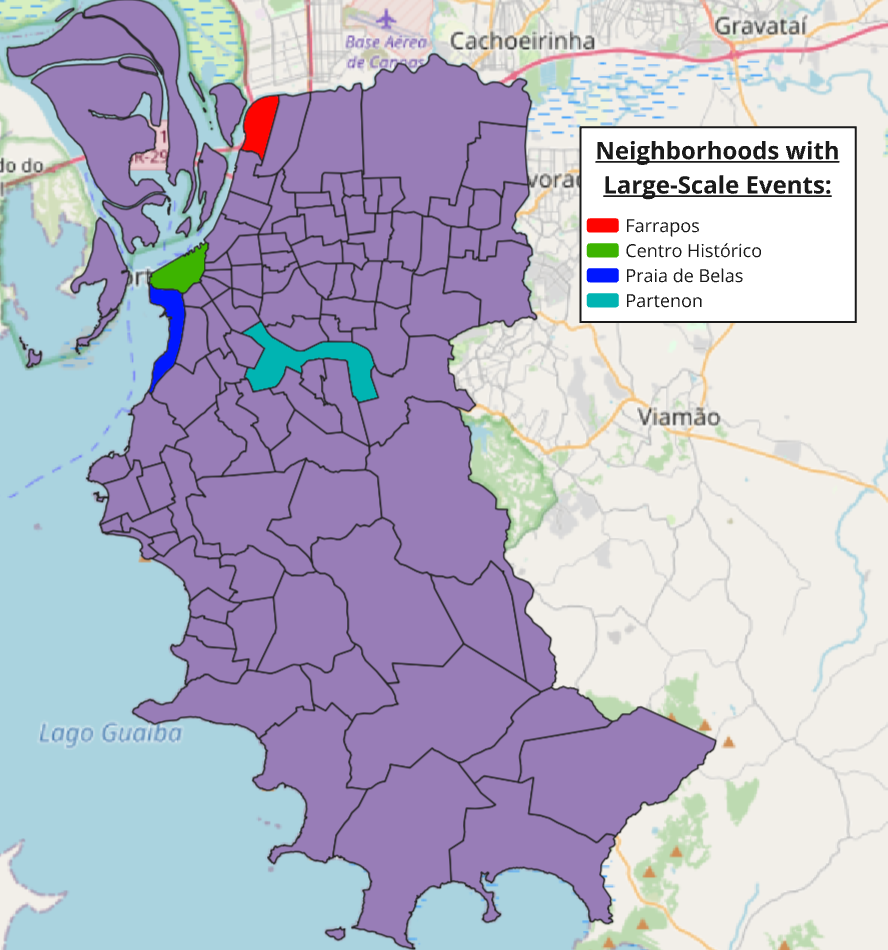
\includegraphics[width=0.6\textwidth]{Figures/CityViewNeighborhoods.png}
  \caption{The 94 neighborhoods of Porto Alegre, Brazil. All 94 neighborhoods of the city are included in all our experiments, with four specific neighborhoods highlighted for their additional routines, utilized in our large-scale experiments (Section~\ref{sec:large_scale}).} 
  \label{fig4:city_view}
\end{figure}

We utilized the OpenStreetMap database~\footnote{OpenStreetMaps is available at: \url{https://www.openstreetmap.org/}} to extract the geographic coordinates (latitude and longitude) of buildings and amenities within Porto Alegre that could serve as points of interest for the population, such as schools and pharmacies.
These points of interest were distributed across the city's neighborhoods. Each region in the model includes the following $P$s: \textit{home}, \textit{work}, \textit{school}, \textit{marketplace}, \textit{pharmacy}, and \textit{gas\_station}. Additionally, some regions may feature other $P$s, such as \textit{shopping\_malls}, \textit{hospitals}, \textit{universities} or \textit{stadiums}.
The modeled environment comprises 94 $R$s and a total of 504 $P$s. For the experiments described in this paper, each region contains at most one $P$ of each type, such as one \textit{home} and one \textit{pharmacy} per neighborhood. This setup was dictated by the available data, which provided information on population distribution at the neighborhood level but did not specify finer-grained details within neighborhoods. However, this is not a limitation of the proposed model. When more granular data is available, simulation designers can enhance the environment by adding multiple home $P$s within a single region and allocating neighborhood populations accordingly. Appendix~\ref{app:input_environment} provides an example of the syntax needed to inform data for modeling an environment in our simulations.

To model the population in our simulations, we collect data from governmental sources, including the most recent completed census at the time of this publication\footnote{Census Conducted by the Brazilian Institute of Geography and Statistics (IBGE). The data is available at:  \url{https://cidades.ibge.gov.br/brasil/rs/porto-alegre/panorama}}. Census data provided citywide information on the total population, the number of economically active individuals (i.e., workers), the number of students, and the age distribution of the population. However, this information lacked specificity at the neighborhood level.
To address this, additional data was gathered from city administration surveys, which included neighborhood-level details on total population and age distribution~\footnote{Surveys conducted by the Observatory of the City of Porto Alegre (ObservaPOA). Data is available at: \url{http://www.observapoa.com.br/}}\footnote{Surveys conducted by the Empresa Pública de Tecnologia da Informação e Comunicação da Prefeitura de Porto Alegre (PROCEMPA). Data is available at: \url{https://portoalegreemanalise.procempa.com.br/}}.
This information was used to define sampled characteristics for the population, with the following identifiers and categories:
\begin{itemize}
    \item $Age$: Child, Young, Adult, and Elder;
    \item $Occupation$: Student, Worker, and Other.
\end{itemize}

Porto Alegre's total population is $1,409,351$. Since \textit{occupation} data was only available at the city level, all neighborhoods were assigned the same distribution: \textit{students} comprise approximately $21.575\%$ of the population, \textit{workers} $54.706\%$, and \textit{other} $23.718\%$.
The \textit{age} distribution was mapped using the age pyramid, with each category representing a specific range: \textit{child} (0–14 years), \textit{young} (15–24 years), \textit{adult} (25–59 years), and \textit{elder} (60+ years). Each neighborhood has its own unique \textit{age} distribution, while the overall population consists of approximately $18.724\%$ \textit{children}, $15.706\%$ \textit{young}, $50.507\%$ \textit{adults}, and $15.061\%$ \textit{elders}. 

For each neighborhood, a blob was initialized at the corresponding \textit{home} $P$, with its total population determined based on the available neighborhood data and its sampled characteristics determined according to the previously described \textit{age} and \textit{occupation} distributions.
Each blob was also assigned a traceable characteristic, \textit{region of origin}, which indicates where the population resides and begins within the simulation. This traceable characteristic enables the identification of a blob's origin throughout the simulation and ensures that the population returns to their respective residences after completing daily activities. Moreover, blobs originating from different regions cannot be merged, as their traceable characteristics remain distinct, preserving information about their place of origin.
Appendix~\ref{app:input_population} provides an example of the input data necessary for modeling an initial population in our simulations.
For all experiments, a \textit{cycle} was defined as 24 \textit{cycle steps}, representing a full day and its hours, respectively. The following sections present results obtained from various simulation scenarios, illustrating the model's capacity to capture population dynamics effectively.




\subsubsection{Census-Sector Environments}
\label{evaluation:spatial}

Table~\ref{tbl:spatial_representations} distinguishes the three principal spatial representations. The original published scenario uses one home per neighborhood. The recent inputs place homes at census-sector locations within regions, so several homes can coexist in a neighborhood. The 13-region environment is a reduced study area used for the flood matrix and reduced dialysis network, while the 94-region environment provides complete-city coverage for selected no-flood mobility, inpatient, and dialysis configurations.

\begin{table}[ht]
\centering
\footnotesize
\caption{Spatial representations used in the thesis. Counts describe the stored environments used by the reported studies.}
\label{tbl:spatial_representations}
\begin{tabularx}{\linewidth}{@{}lrrX@{}}
\toprule
\textbf{Representation} & \textbf{Regions} & \textbf{Home nodes} & \textbf{Purpose} \\ \midrule
Original neighborhood scenario & 94 & 94 & Published random-walk, large-event, epidemic, and performance experiments; one aggregated home per neighborhood. \\ \midrule
Reduced census-sector scenario & 13 & 435 & Flood and adaptation matrix and reduced dialysis experiments; multiple home nodes per region. \\ \midrule
Complete census-sector scenario & 94 & 2,711 & Complete-city inpatient and dialysis configurations and the no-flood Popular Times evaluation. \\ \bottomrule
\end{tabularx}
\end{table}

The finer representation changes scenario inputs and the distances from which populations may be selected; it does not alter the definitions of regions, points of interest, blobs, templates, or actions. Domain inputs add hospitals, dialysis clinics, water-treatment facilities, workplaces, schools, marketplaces, restaurants, and pharmacies as ordinary points of interest with type-specific attributes consumed by plugins.



\subsection{Population, Facilities, and External Data}
The census-sector population files allocate residents to home nodes and retain population characteristics used by movement plugins. The original and recent experiments therefore use the same population abstraction at different input granularities. Popular Times V2 combines initial home populations with fixed weekly hourly profiles for marketplaces, restaurants, and pharmacies. Levy Walk V2 allocates worker and student attendance targets across work and school destinations and divides movements into packets of at most 50 people.

The inpatient environment incorporates hospital locations and January 2024 bed-capacity data derived from the LODUS-Health CNES dataset~\citep{souza2026lodushealth}. Capacity is separated into public (SUS) and private pools. The dialysis inputs add clinics, opening schedules, treatment capacities, and water-treatment nodes. Demand magnitudes, recovery schedules, facility allocations, and routing mappings are experiment configuration, even when facility locations or capacities originate in an external dataset.

The flood experiments use the repository's time-indexed water-level series and node exposure attributes. At each step, the flood plugin may add or remove a flood disable cause. This design keeps the environmental observation, the threshold that maps it to availability, and the movement response as separate layers.



\subsubsection{Disruption and Dependency Inputs}
Direct availability changes cover scheduled closures, experiment-specific outages, and flood exposure. Every cause is tracked independently. Dependency rules are then evaluated using the effective states defined in Equation~\ref{eq:node_availability}. In the dialysis scenarios, clinics can depend on water-treatment facilities selected through shared attributes. Disabling a required facility propagates a dependency blocker to the clinic; restoring one direct cause does not remove unrelated blockers.

Availability does not automatically move population. The dialysis plugin excludes disabled clinics from admission, the inpatient plugin can use an enabled fallback, Popular Times V2 can suppress or reroute visits, and Levy Walk V2 records unavailable origins, unavailable destinations, temporary returns, blocked returns, and repatriation. This division allows the same node-state mechanism to support different domain responses.



\subsection{Scenario Time Semantics}
The mobility and dialysis studies use 24 hourly steps per daily cycle. Popular Times and Levy Walk V2 run for 56 days, whereas the dialysis catalog runs for 10 days. Inpatient care uses 12 abstract admission/discharge steps arranged as three cycles of four; those steps should not be interpreted as hours. 

Hourly steps therefore indicate clock time only in the mobility and dialysis families. The inpatient steps encode admission and discharge intervals defined by that experiment. Cross-study interpretation uses each family's own temporal unit rather than converting unlike intervals into a common rate.

\subsection{Replications, Metrics, and Validation}
Table~\ref{tbl:extended_batches} summarizes the completed experiment batches. Matched seeds reduce unrelated stochastic variation when two configurations are compared. Deterministic configurations are run once and are not assigned artificial confidence intervals. Repeated stochastic conditions are summarized by their reported means and 95\% intervals.

\begin{table}[ht]
\centering
\footnotesize
\caption{Recent experiment batches included in the thesis.}
\label{tbl:extended_batches}
\begin{tabularx}{\linewidth}{@{}lrrX@{}}
\toprule
\textbf{Batch} & \textbf{Scenarios} & \textbf{Runs} & \textbf{Principal outcomes} \\ \midrule
Inpatient care & 7 & 210 & Coverage, overflow, queue length, admission delay, specialty/payer service, and distance. \\ \midrule
Dialysis resilience & 12 & 361 & Treatment coverage, overdue demand, waiting exposure, admission distance, and disabled clinic-hours; one extra K03 record is retained. \\ \midrule
Popular Times V2 core & 10 & 130 & Visit fulfillment, travelers, distance, occupancy, population conservation, and node-state validity. \\ \midrule
Destination adaptation & 2 & 31 & Rerouted and unmet visits, added displacement, receiving load, and fulfillment. \\ \midrule
Levy Walk V2 & 5 & 150 & Commute fulfillment, unmet reasons, moved population, distance, return lifecycle, and activity-visit fulfillment. \\ \bottomrule
\end{tabularx}
\end{table}


Validation includes population conservation, enabled-node movement checks, exact cycle-level attendance where specified, demand accounting, and specialized integrity checks. All 130 Stage 4, 31 Stage 5, and 150 Stage 6 mobility runs passed their respective invariants; the inpatient package passed 2,052 integrity checks and five determinism checks.



\subsection{Data Provenance and Modeling Assumptions}
Observed, derived, and synthetic inputs are reported separately. Geographic locations, census-sector population inputs, hospital capacities, and the water-level series provide empirical context, subject to their collection dates and preprocessing. Visit rates, demand profiles, outage schedules, thresholds, recovery times, synthetic facilities, CID mappings, and some routing allocations are model configurations. In particular, the synthetic Santa Ana capacity and the CID-based inpatient demonstration are not observations of clinical practice.

Stochastic repetitions quantify variability produced by the implemented sampling process, not uncertainty in every input parameter. Some demand components are deterministic and therefore produce identical fulfillment values across seeds. External validity requires calibration and comparison with observed mobility or service data and is discussed in Section~\ref{discussion:validity}.

The numerical tables in Sections~\ref{sec:health_resilience} and \ref{sec:flood_mobility} are transcribed from the preserved repository summaries: \texttt{results/dialysis/analysis/scenario\_summary.csv}, \texttt{results/inpatient\_care/analysis/report.md}, \texttt{docs/results/popular\_times\_v2\_stage4/REPORT.md}, \texttt{docs/results/popular\_times\_v2\_stage5/REPORT.md}, and \texttt{output\_logs/popular\_times\_v2\_stage6/REPORT.md}. Raw run directories and metadata remain the audit sources when an alternative aggregation is required.



\section{Routine Mobility and Spatial Granularity}
\label{sec:routine_mobility}

\subsection{Neighborhood-Level Baseline Scenario}

The original neighborhood-level environment and population are defined in Section~\ref{sec:case_scenario}. This first evidence family asks whether routines and plugins can generate interpretable movement from aggregated homes before introducing census-sector origins or infrastructure disruption. The original published numerical results are reproduced without retrospective modification.

\subsection{Original Levy Random-Walk Experiment}
\label{sec:random_walk}

Gonzalez et al.~\citep{gonzalez2008understanding} provide valuable insights into the dynamics of urban populations, which serve as a foundation for our abstracted urban mobility model. They highlight two significant observations: first, individuals tend to visit a select few locations repeatedly, and second, there is a certain level of randomness in their daily movements, akin to a Lévy flight random walk.
A Lévy flight is a random walk pattern characterized by jumps of varying lengths, following a Lévy heavy-tailed probability distribution. In practical terms, this means that the Lévy flight predominantly consists of short jumps, with fewer long jumps.

To simulate this behavior, we have implemented a Lévy plugin, which introduces a new action type called the \textit{levy walk}. Appendix~\ref{app:plugin} presents an example of how new action types can be incorporated into our simulations using plugins. This action involves sampling distances from a Lévy distribution and moving a certain portion of the population from a certain origin $P_i$ to a destination $P_j$ corresponding to the sampled distance.
For each $P$, we calculate a histogram of distances to other $P$s, grouping them into bins based on a specified distance grouping value. Figure~\ref{fig5:node_distances} illustrates the histogram of distances between $P$s, with each bin representing a range of 500 meters.

\begin{figure}[ht]
 \centering
  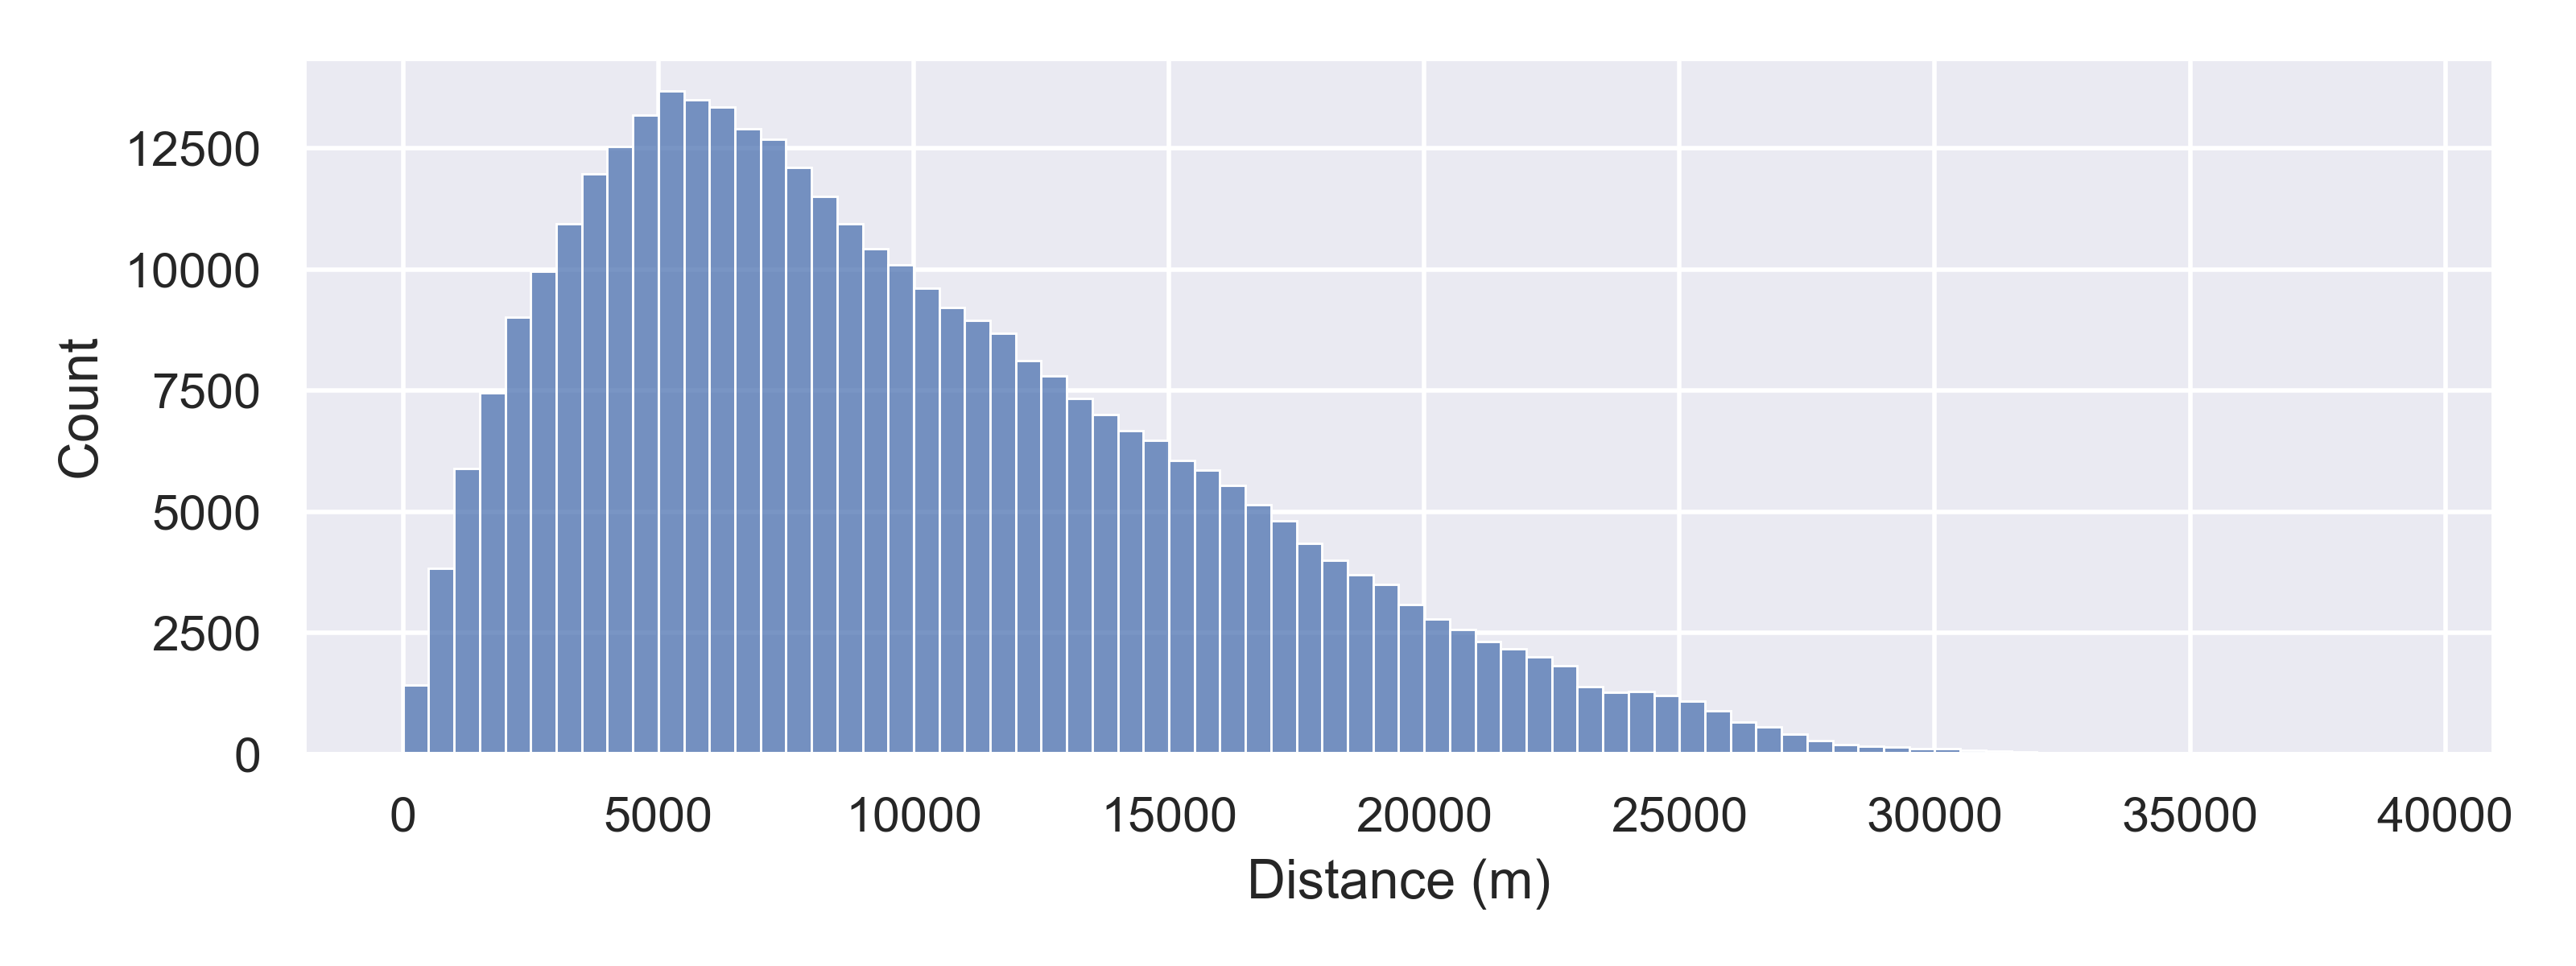
\includegraphics[width=0.95\textwidth]{Figures/NodeDistances.png}
  \caption{ Histogram of distances between points of interest ($P$s). Each bin represents a range of 500 meters.} 
  \label{fig5:node_distances}
\end{figure}

When the \textit{levy walk} action is triggered, the population at the origin $P_i$ is uniformly divided into packets to be moved. Upon sampling a distance, the \textit{levy walk} action randomly assigns a population packet to one of the $P$s within that distance group. Since the Lévy distribution is heavy-tailed (see Figure~\ref{fig6:levy_distributions}), it is possible to sample a distance that exceeds the farthest $P$, even if it is not very probable. In such cases, another distance is sampled from the distribution. Similarly, if there are no available $P$s within the sampled distance group, a new distance will be sampled.

A \textit{levy walk} action $A_i$ incorporates additional parameters $\bm{V}_{i}$ (Section~\ref{sec:routines}) to enhance its functionality. These parameters include the scale parameter ($levy\_scale$), which governs the Lévy distribution; the movement probability parameter ($levy\_prob$), which determines the likelihood of a population packet being moved; the packet size parameter ($levy\_pkt$), representing the group size that undergoes the random walk; and an optional label parameter ($levy\_label$), enabling the selection of specific types of $P$s as potential destinations. 
Additionally, a \textit{levy walk} action $A_i$ requires a population template $T_{i}$ to specify the desired population profile being affected.
These parameters enable the simulation of random walk behavior across multiple scales: spatial scales, by adjusting the $levy\_scale$ parameter to match the simulated environment, and population scales, by modifying $levy\_pkt$, which allows for the movement of large populations or individual entities (i.e., a blob with a total population of 1).

In our experiments, we design a global routine ($GRo$) that utilizes \textit{levy walk} actions to disperse the working and student populations across the city throughout the day. Actions targeting workers relocate the population from a ``home" $P_h$ to a ``work" $P_w$, utilizing a population template with criteria such as $Occupation = Worker$ and $Age = [Young, Adult, Elder]$. These actions occur at each cycle step, with a higher movement probability ($levy\_prob$) during the morning and afternoon (specifically, steps 7 through 18).
Actions targeting students relocate the population from a ``home" $P_h$ to a ``school" $P_s$, using a population template with criteria such as $Occupation = Student$ and $Age = [Child, Young, Adult]$. These actions are executed only at specific cycle steps. Furthermore, the simulation routine includes \textit{move population} actions in all ``work" and ``school" $P$s, returning a portion of their current population to their respective ``home" $P$ of each blob they contain. In both cases, the \textit{region of origin} traceable characteristic of each blob allows us to identify the ``home'' $P$s where students and workers originate and return at the end of the day.

Subsequently, we conducted experiments by varying the $levy\_scale$ parameter in all \textit{levy walk} actions to assess the population movements throughout the simulation. We define ``displacement" as the movement of an individual from one $P_i$ to another $P_j$, as part of the levy plugin.
In the case of a blob $B_i$ with a total population $TP_i = 250$, each movement between points of interest accounts for 250 displacements. All simulations maintain a population packet size of $levy\_pkt = 250$, and the $P$s are grouped based on the distance to an origin $P$, with intervals of 500 meters, as depicted in Figure~\ref{fig5:node_distances}.

The experimental results are illustrated in Figure~\ref{fig6:levy_distributions}. All simulations consider a total population of $1,409,351$. The x-axis represents the distance traveled during each displacement, grouped into 500-meter intervals.
The y-axis indicates the total number of displacements that occurred at each levy configuration. The graph demonstrates that different values of the $levy\_scale$ parameter produce distinct distributions, where higher values yield more widely dispersed distributions of displacements, as observed in a simulation where $levy\_scale = 10$.

\begin{figure}[ht]
 \centering
  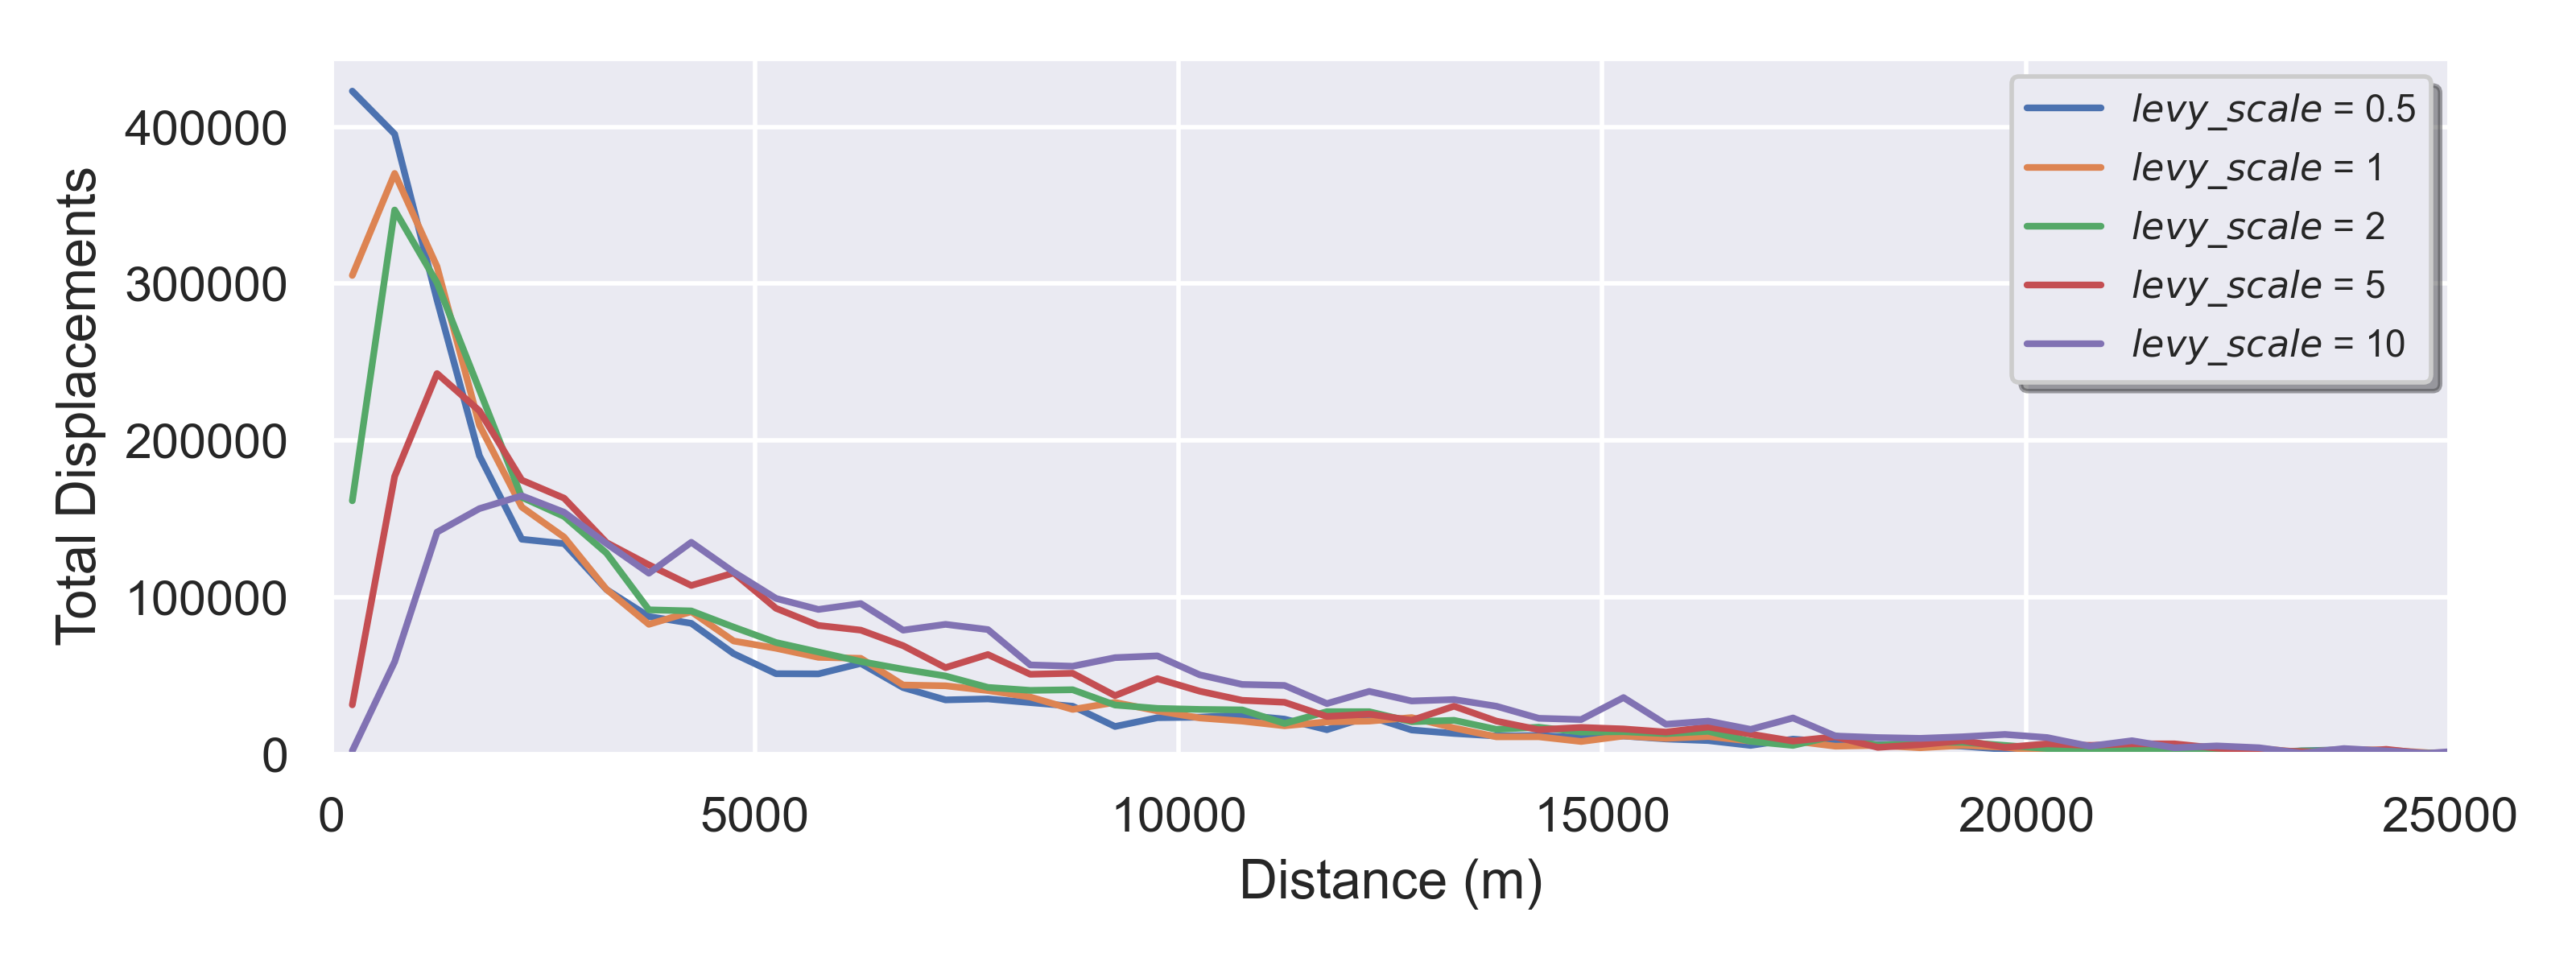
\includegraphics[width=0.95\textwidth]{Figures/Levy_Distributions.png}
  \caption{ Population displacement experiments. The x-axis represents the distance traveled during a displacement and is grouped in ranges of 500 meters. The y-axis represents the total number of displacements that traveled a certain distance. All simulations consider a total population of $1,409,351$; a population packet size of $levy\_pkt = 250$, which represents the group size that undergoes the random walk; and $P$s grouped by distance in ranges of 500 meters, as presented in Figure~\ref{fig5:node_distances}.} 
  \label{fig6:levy_distributions}
\end{figure}
%python .\movement_displacement_comparison.py --p levy_parameter_tests_94 --b 500 --e WorkSchool94-BW_500-S_250  WorkSchool94-BW_500-S_500 WorkSchool94-BW_500-S_1000  WorkSchool94-BW_500-S_2500 WorkSchool94-BW_500-S_5000 --x 25000 --l "Scale = 0.5" "Scale = 1" "Scale = 2" "Scale = 5" "Scale = 10"

For the remaining experiments in this work, we adopt a scale parameter of $levy\_scale = 2$ (represented by the green line in Figure~\ref{fig6:levy_distributions}). This particular value was determined empirically, as approximately $50\%$ of the displacements observed in simulations using this parameter occurred within a 2km radius of the origin $P$. Such displacements align with typical daily movements within a single neighborhood or between neighboring neighborhoods. However, this value can be adjusted to suit different environments, depending on the needs of the simulation designers. 

Furthermore, we introduce an additional parameter, named $Restriction$, for the \textit{levy walk} action to model movement restrictions.
This parameter acts as a factor that reduces the total population being moved by each \textit{levy walk} action, e.g., an $Restriction = 0.25$ would cause a \textit{levy walk} action to move only $\approx75\%$ of the population it would without the restriction. It allows for the simulation of varying population flows on different days of the week (e.g., weekends with different flow patterns than weekdays) or the simulation of population lockdown during a pandemic scenario. Figure~\ref{fig7:movement_restriction} illustrates the results obtained by conducting a baseline experiment (without any restriction) and three other experiments involving different levels of movement restrictions. As previously mentioned, all simulations consider a scale parameter of $levy\_scale = 2$.

\begin{figure}[ht]
 \centering
  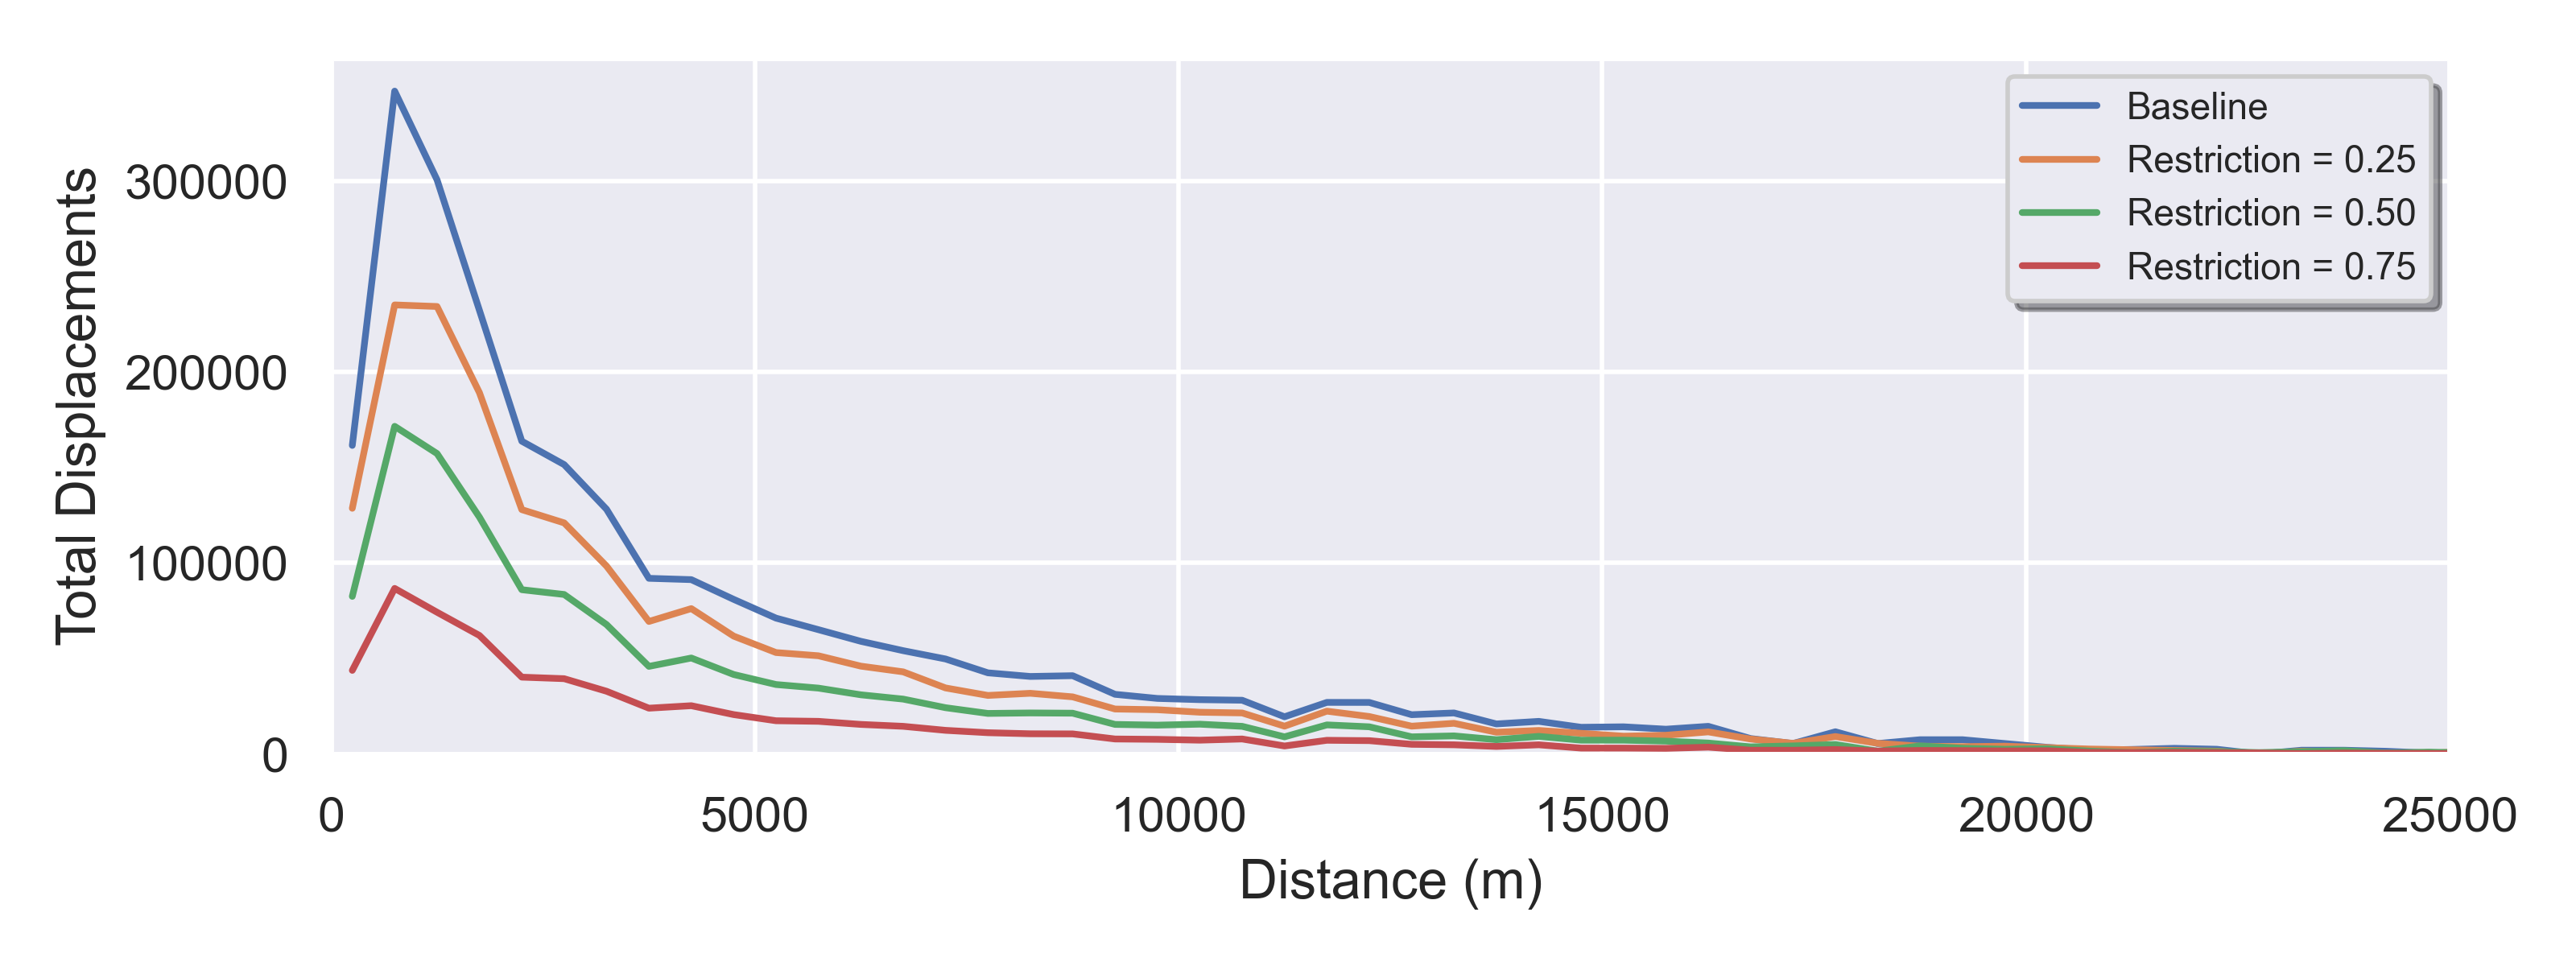
\includegraphics[width=0.98\textwidth]{Figures/MovementRestriction.png}
  \caption{Simulation of Movement Restriction with the \textit{levy walk} action. All simulations consider a scale parameter of $levy\_scale = 2$. The $Restriction$ parameter acts as a factor that reduces the total population being moved by each \textit{levy walk} action.} 
  \label{fig7:movement_restriction}
\end{figure}
%python .\movement_displacement_comparison.py --p isolation_tests --b 500 --e Baseline Baseline-Iso_25 Baseline-Iso_50 Baseline-Iso_75 Baseline-Iso_100 --l Baseline "Restriction = 0.25" "Restriction = 0.50" "Restriction = 0.75" "Restriction = 1.00" --x 25000




\subsection{Census-Sector Mobility and Popular Times}
Popular Times V2 models weekly hourly visits to marketplaces, restaurants, and pharmacies. Demand is derived from the initial population associated with each home node and fixed weekly profiles. Travelers are sourced from enabled homes, occupy a destination for one hour, and then return to their prior node. The reduced environment contains 13 regions and 435 census-sector homes; the complete environment contains 94 regions and 2,711 homes.

The flood schedule can affect homes, activity points of interest, or both. A disabled home is not used as a source, while a disabled destination either suppresses its request or, in the adaptation condition, redirects it to the nearest enabled point of interest of the same type. Legacy Levy movement can be enabled alongside these visits to change the population distribution from which travelers are sourced.



\subsection{Popular Times Baseline Results}

The Stage 4 no-flood baseline separates scheduled activity demand from flood response. In the reduced 13-region Levy-on configuration, all requested visits are fulfilled, with 17.9997 travelers per capita and a mean sourcing-distance measure of 81.9953 per request. The deterministic Levy-off configuration also achieves complete fulfillment. The five-seed complete 94-region no-flood evaluation likewise achieves complete fulfillment, demonstrating that the same visit mechanism operates with 2,711 census-sector home nodes. Flooded conditions from the same matrix are examined in Section~\ref{sec:flood_mobility} because they test environmental disruption rather than baseline demand generation.

\subsection{Commuting and Levy Walk V2 Baseline}

Levy Walk V2 changes the mobility question from opportunistic movement to explicit worker and student attendance. Cycle-level targets are allocated across census-sector homes and assigned work or school destinations, with movements divided into packets of at most 50 people. In the no-flood Stage 6 condition, commute fulfillment is 100%, mean commute distance is 1,393.53~m, and Popular Times activity fulfillment is also 100%. The full disruption and return lifecycle is evaluated in Section~\ref{sec:flood_mobility}.

\subsection{Mobility and Resolution Synthesis}

The original Levy experiment demonstrates configurable stochastic displacement from neighborhood aggregates, whereas Popular Times introduces scheduled activity demand from census-sector homes and Levy Walk V2 introduces assigned attendance. Together they show that spatial refinement changes origins and possible distances without changing the blob representation. They do not establish that one movement rule is behaviorally superior: the mechanisms answer different questions and rely on different input assumptions.

\section{Demand Shocks and Population-State Interventions}
\label{sec:interventions}

\subsection{Extension Mechanisms}

The original event and epidemic studies demonstrate two distinct plugin patterns. A demand shock changes which locations request population and when, while a state intervention changes traceable characteristics that affect later actions. Both operate through the same action, template, split, merge, and routine interfaces defined in Section~\ref{sec:proposed_model}.

\subsection{Large-Scale Event Scenarios}
\label{sec:large_scale}

We also investigate the ability to simulate occasional events that disrupt the population's daily routines, such as sports matches or musical concerts that occur on a weekly or monthly basis.
To evaluate the impact of these large-scale events on mobility patterns, we compare their effects against a baseline scenario with no events. Furthermore, we examine how multiple concurrent events compete for the available population, highlighting the dynamics of population distribution.

To simulate these events, we implemented an additional plugin, which introduces a new action type called \textit{gather population}. This action involves gathering the population from nearby $P$s and relocating them to a designated destination $P_d$. 
A \textit{gather population} action $A_j$ considers a $gather\_quantity$ additional parameter (in $\bm{V}_{j}$)  to describe the total population to be relocated towards the destination $P_d$. 
The population quantity to be moved from each nearby $P$ is determined by the population available at the origin $P$ and the distance to the destination.
Once the population quantity that should be moved from each origin $P$ is determined, the \textit{gather population} action is further broken down into multiple \textit{move population} actions. Each of these \textit{move population} actions is responsible for transferring the population from an origin $P$ to the destination $P_d$, ensuring that each origin $P$ contributes to the movement.

For these experiments, we consider the routines of workers and students as a baseline simulation, utilizing a scale parameter of $levy\_scale = 2$ as described in Section~\ref{sec:random_walk}.
Furthermore, we incorporate four large-scale events into the simulation, each occurring at a specific cycle step. These events are characterized by a \textit{gather population} action, which requests the movement of 500,000 individuals to a designated destination $P$. The details of the events are specified as follows, considering the regions illustrated in Figure~\ref{fig4:city_view}: 

\begin{itemize}
    \item Event $(A)$: A sports event taking place at the Farrapos region stadium;
    \item Event $(B)$: A sports event happening at the Praia de Belas region stadium;
    \item Event $(C)$: A commercial event held at the marketplace in the Centro Histórico region; and
    \item Event $(D)$: A cultural event occurring at our University in the Partenon region.
\end{itemize}

All events are scheduled to occur at cycle step 19, i.e., at 7:00 PM. Given that the city's total population is 1,409,351, and the events require a total of 2,000,000 individuals, the events will compete for the available population if they all occur simultaneously in a single simulation.
In addition, we model a scenario where some large-scale events take place at different cycle steps. In this alternate scenario, event C occurs at cycle step 9 (i.e., 9:00 AM), while event D occurs at cycle step 14 (i.e., 2:00 PM).

Table~\ref{tbl:results_displacement} provides an overview of the simulation results, including the total population displacements, the average displacement per city inhabitant, and the proportion of total displacements compared to the baseline simulation. Baseline means the ``normal life'' of the city, and the different scenarios in the table indicate the population displacements as a function of the existence of the events. For instance, the ``Baseline+AB'' scenario considers the Baseline in addition to Event A and Event B. In the two last lines of Table~\ref{tbl:results_displacement}, we show the results of the Baseline with the existence of the four large-scale events occurring at the same time and with some occurring at different cycle steps.


\begin{table}[ht]
\footnotesize
\centering
\caption{Results of the large-scale event simulations. Data includes the total population displacements, the average displacement per inhabitant of the city, and a proportion of total displacements compared to the baseline simulation. The ``Baseline+AB'' scenario, for example, considers the Baseline in addition to Event A and Event B.}
\label{tbl:results_displacement}
\begin{tabular}{@{}lccc@{}}
\toprule
Experiment Name        & \begin{tabular}[c]{@{}c@{}}Total\\ Displacements\end{tabular} & \begin{tabular}[c]{@{}c@{}}Average Displacements\\ per inhabitant\end{tabular} & \begin{tabular}[c]{@{}c@{}}Increase over\\ Baseline\end{tabular}  \\ \midrule
Baseline               & 2,570,658                                                                                                                                                 & 1.8240                                                                                                                                                 & ---             \\ \midrule
Baseline+A             & 3,290,469                                                                                                                                                 & 2.3347                                                                                                                                                 & 28.00\% \\ %1.2800           \\
Baseline+B             & 3,300,782                                                                                                                                                 & 2.3421                                                                                                                                                 & 28.40\% \\ %1.2840           \\
Baseline+C             & 3,289,002                                                                                                                                                 & 2.3337                                                                                                                                                 & 27.94\% \\ %1.2794           \\
Baseline+D             & 3,281,102                                                                                                                                                 & 2.3281                                                                                                                                                 & 27.64\% \\ \midrule %1.2764           \\ \midrule
Baseline+AB            & 3,786,856                                                                                                                                                 & 2.6870                                                                                                                                                 & 47.31\% \\ %1.4731           \\
Baseline+AC            & 3,748,417                                                                                                                                                 & 2.6597                                                                                                                                                 & 45.82\% \\ %1.4582           \\
Baseline+AD            & 3,804,017                                                                                                                                                 & 2.6991                                                                                                                                                 & 47.98\% \\ %1.4798           \\
Baseline+BC            & 3,738,497                                                                                                                                                 & 2.6526                                                                                                                                                 & 45.43\% \\ %1.4543           \\
Baseline+BD            & 3,839,126                                                                                                                                                 & 2.7240                                                                                                                                                 & 49.34\% \\ %1.4934           \\
Baseline+CD            & 3,826,094                                                                                                                                                 & 2.7148                                                                                                                                                 & 48.84\% \\ \midrule %1.4884           \\ \midrule
Baseline+ABC           & 4,042,413                                                                                                                                                 & 2.8683                                                                                                                                                 & 57.25\% \\ %1.5725           \\
Baseline+ABD           & 4,109,929                                                                                                                                                 & 2.9162                                                                                                                                                 & 59.88\% \\ %1.5988           \\
Baseline+ACD           & 4,069,223                                                                                                                                                 & 2.8873                                                                                                                                                 & 58.29\% \\ %1.5829           \\
Baseline+BCD           & 4,081,563                                                                                                                                                 & 2.8961                                                                                                                                                 & 58.78\% \\ \midrule %1.5878           \\\midrule
Baseline+ABCD          & 4,235,926                                                                                                                                                 & 3.0056                                                                                                                                                 & 64.78\% \\ %1.6478           \\ 
Baseline+ABCD+DiffStep & 4,638,329                                                                                                                                                 & 3.2911                                                                                                                                                 & 80.43\% \\ \bottomrule %1.8043           \\ \bottomrule
\end{tabular}
\end{table}



Figure~\ref{fig8:results_displacements} presents the results of the simulation of large-scale events.
Figure~\ref{fig8a:results_displacement_single} visualizes the results of five simulations: the Baseline simulation (no events), a simulation with only Event A, a simulation with only Event B, only Event C, and only Event D. 
As indicated by the data in Table~\ref{tbl:results_displacement}, simulations where only a single large-scale event occurs yield a similar number of total displacements. However, the different locations where each event occurred (i.e., different destination $P$s) and the available population nearby cause each simulation to have other total displacement counts for different distances. For example, the ``Baseline+A'' simulation (shown in orange in Figure~\ref{fig8a:results_displacement_single}) presents an increased total displacement count near the $20,000m$ distance.

\begin{figure}[!htbp]
  \centering
  \subfloat[Experiments include the Baseline scenario (no events), a scenario with only Event A, only Event B, only Event C, and only Event D.]
  {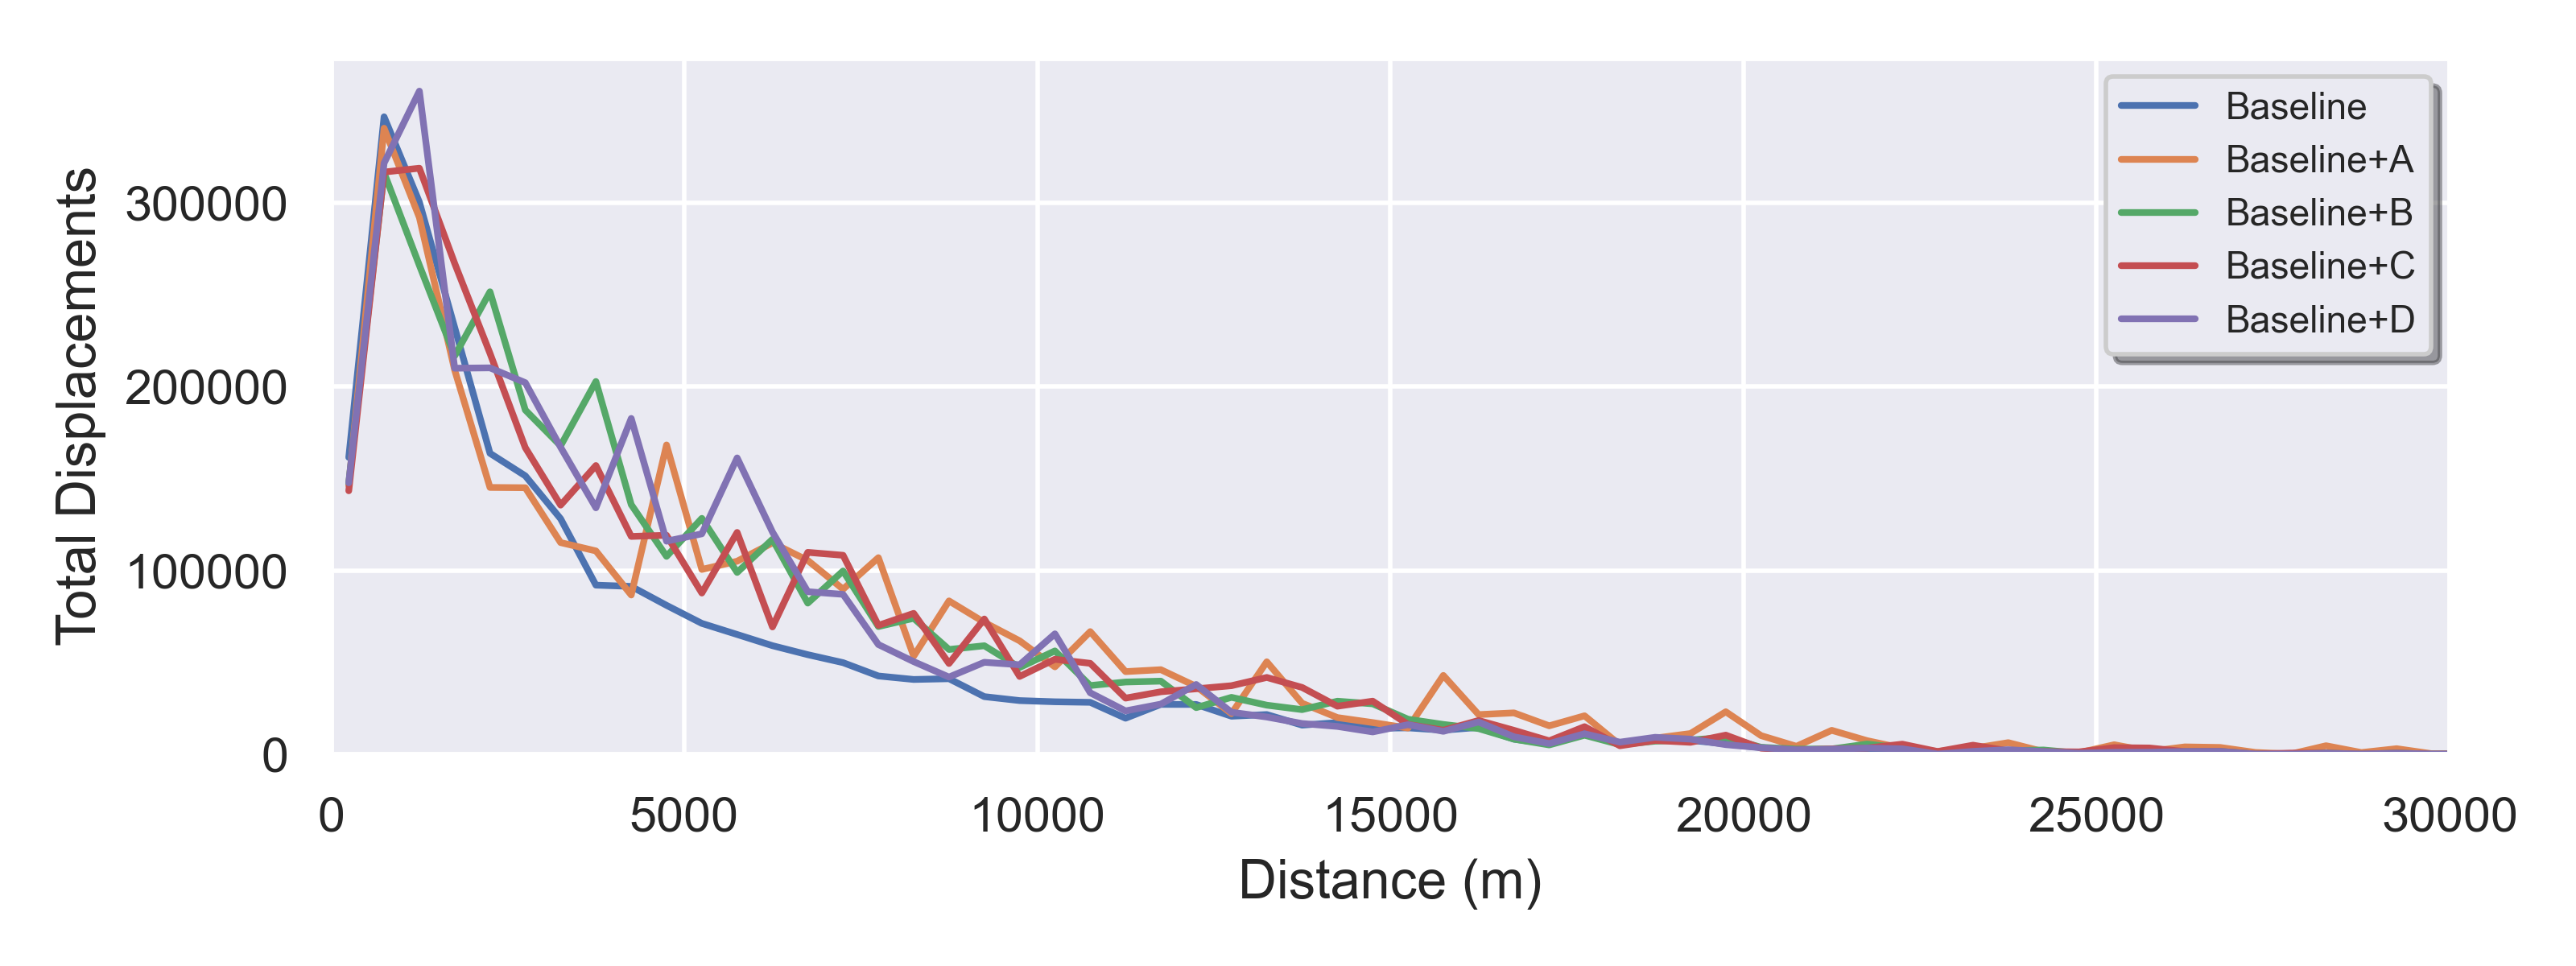
\includegraphics[width=0.95\textwidth]{Figures/Displacement_SingleEvent.png}
  \label{fig8a:results_displacement_single}}\\
  %python .\movement_displacement_comparison.py --p large_scale_event --b 500 --e Baseline Baseline+A_Dist Baseline+B_Dist Baseline+C_Dist Baseline+P_Dist --l Baseline Baseline+A Baseline+B Baseline+C Baseline+D --x 30000
  \subfloat[Experiments include the Baseline scenario and four other scenarios with three events occurring at the same cycle step (i.e., only one event missing in each).]
  {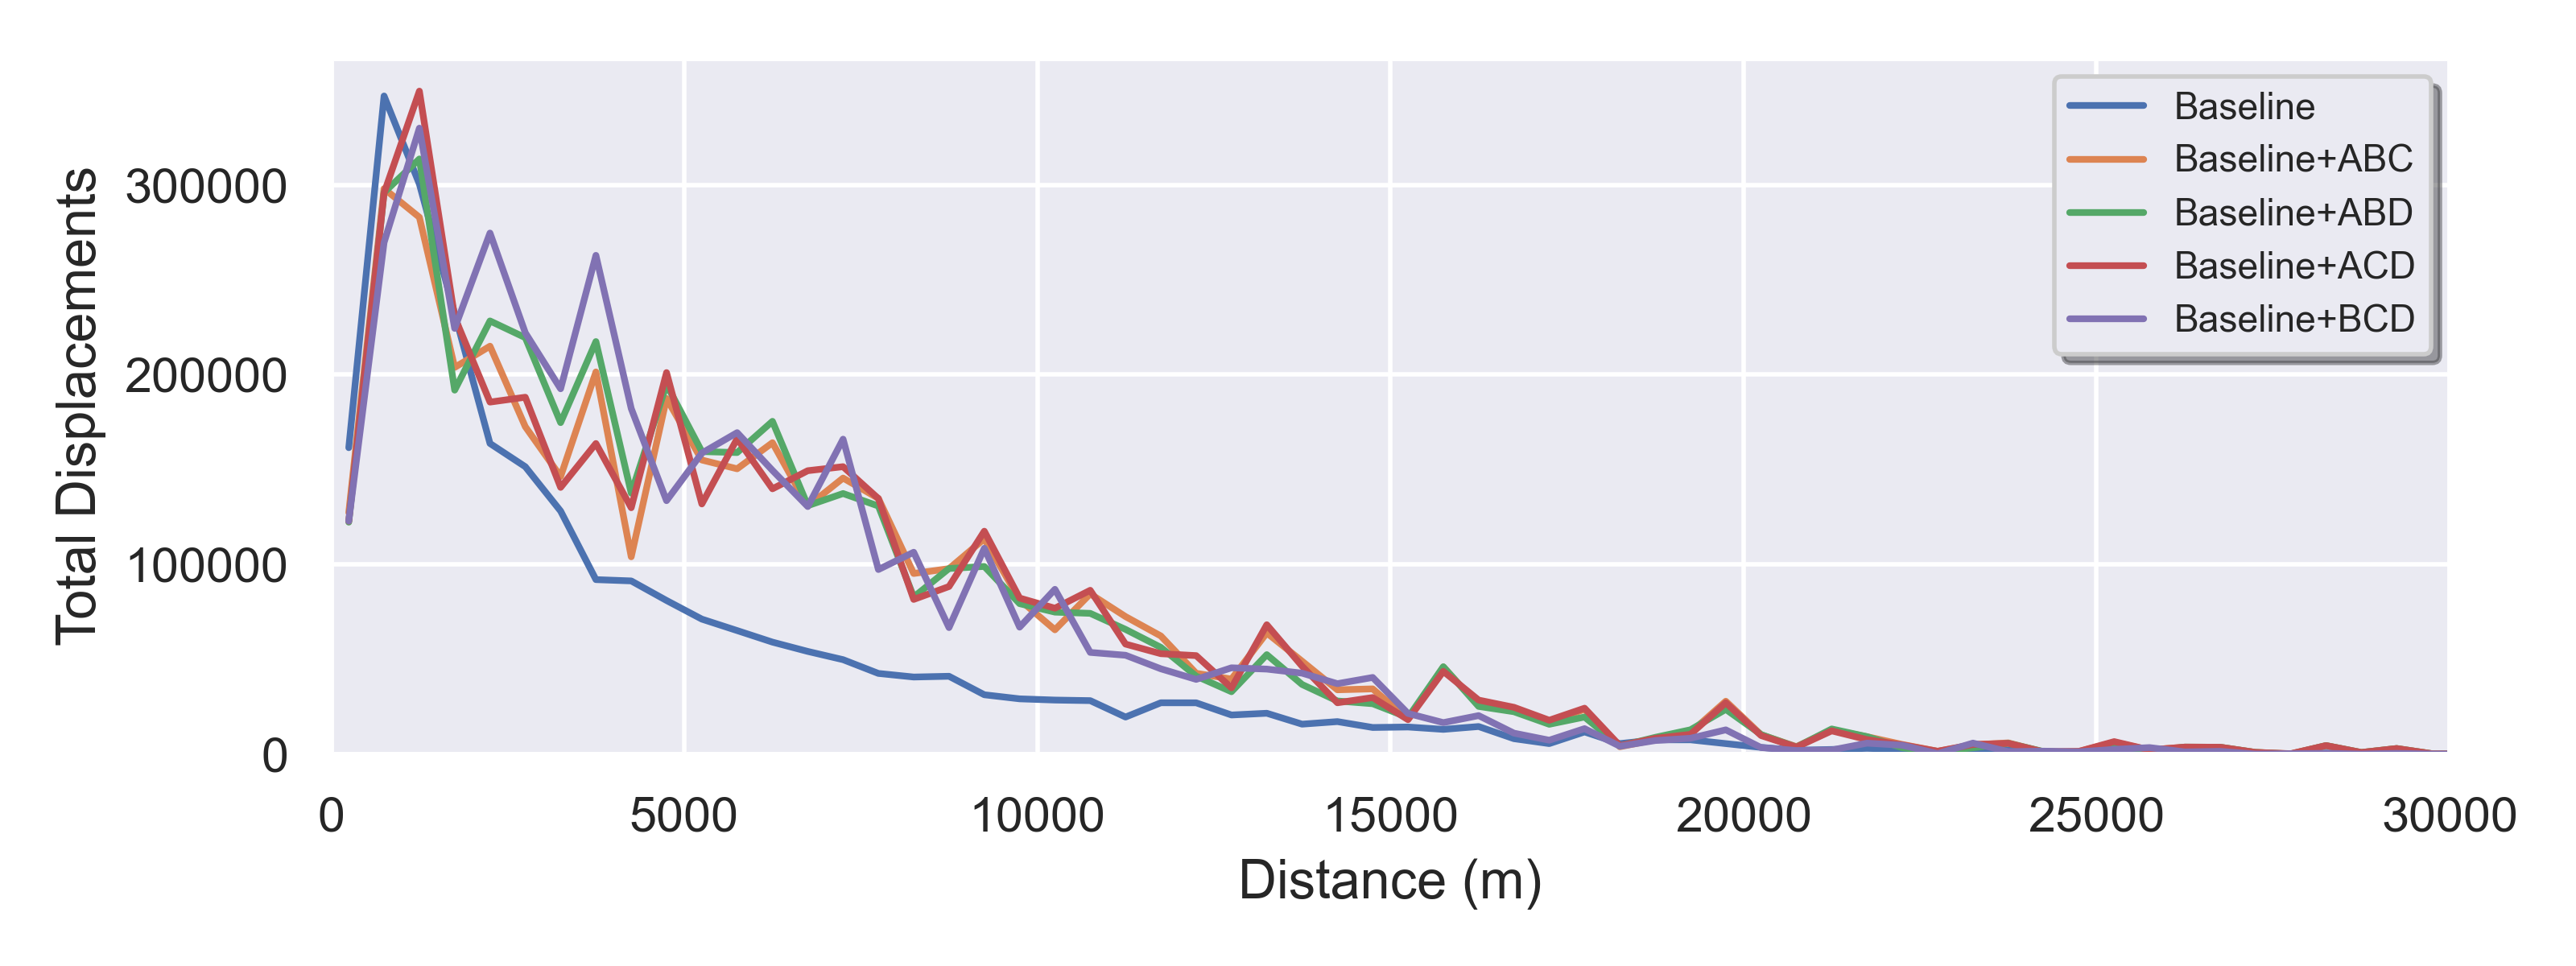
\includegraphics[width=0.95\textwidth]{Figures/Displacement_ThreeEvents.png}
  %python .\movement_displacement_comparison.py --p large_scale_event --b 500 --e Baseline Baseline+ABC_Dist Baseline+ABP_Dist Baseline+ACP_Dist Baseline+BCP_Dist --l Baseline Baseline+ABC Baseline+ABD Baseline+ACD Baseline+BCD --x 30000
  \label{fig8b:results_displacement_three}}\\
  \subfloat[Experiments include the Baseline scenario, the Baseline in addition to all four events occurring at the same cycle step, and the Baseline in addition to all four events with some occurring at different cycle steps (DiffStep).]
  {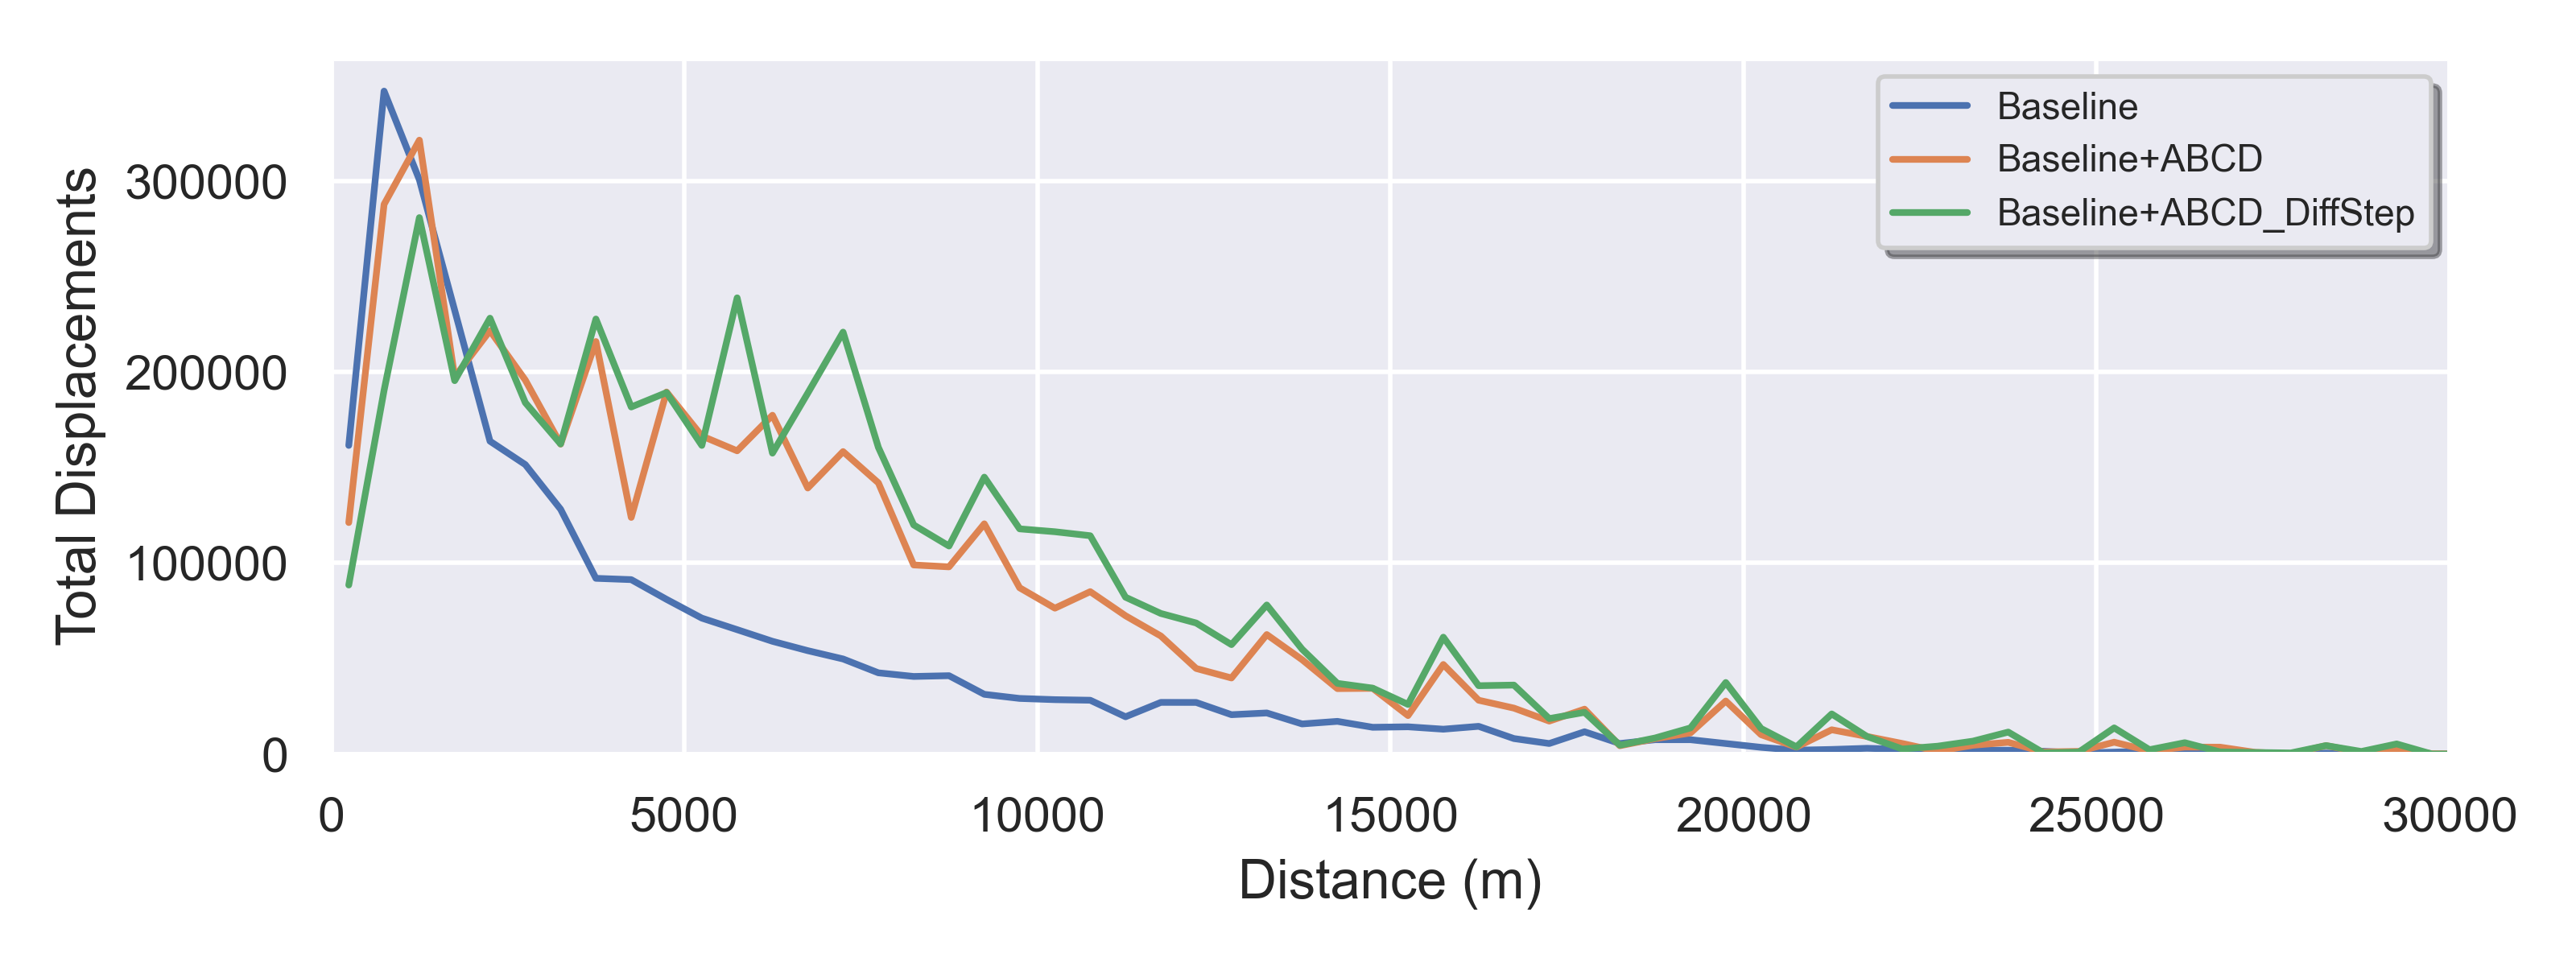
\includegraphics[width=0.95\textwidth]{Figures/Displacement_AllEvents.png}
  \label{fig8c:results_displacement_all}}
  %python .\movement_displacement_comparison.py --p large_scale_event --b 500 --e Baseline Baseline+ABCP_Dist Baseline+DiffStep_ABCP_Dist --l Baseline Baseline+ABCD Baseline+ABCD_DiffStep --x 30000
  \caption{Simulation of large-scale events.}
 \label{fig8:results_displacements}
\end{figure}

Figure~\ref{fig8b:results_displacement_three} illustrates the results of five simulations, starting with the baseline simulation and followed by simulations with three events occurring at the same cycle step (i.e., only one event missing in each). 
As expected, and as indicated by the data in Table~\ref{tbl:results_displacement}, the inclusion of additional events led to an increase in total displacements compared to the baseline simulation. However, it is important to note that although each event requests the movement of 500,000 individuals, the total displacements of three events do not increase by 1,500,000 compared to the baseline simulation. This is because individuals can move directly from their respective origin $P$s (such as work or school) to the event $P$s. Thus, workers can travel from their ``work" $P$s to the event directly, and students can travel from their ``school" $P$s to the event without the need to return to their ``homes" before going to the events. Moreover, Events A, B, and C separately contribute to $\approx730,000$ additional displacements to the baseline simulation, as shown in ``Baseline+A", ``Baseline+B", and ``Baseline+C" in Table~\ref{tbl:results_displacement}, respectively.
In simulations where the three events occur simultaneously (i.e., ``Baseline+ABC''), the events will compete for the available population in nearby neighborhoods, resulting in a reduced total population attending each event. Such result is presented in the last column of Table~\ref{tbl:results_displacement}, where the number of displacements increased over the baseline is $57.25\%$ for simulation ``Baseline+ABC''. This is a lower amount than the sum of increased displacements of simulations ``Baseline+A", ``Baseline+B", and ``Baseline+C", which were $28.00\%$, $28.40\%$, and $27.94\%$, respectively.

Figure~\ref{fig8c:results_displacement_all} presents the results of three simulations: the baseline simulation, a simulation with all four events occurring simultaneously, and a simulation with some events taking place at different cycle steps. As demonstrated by the data in Table~\ref{tbl:results_displacement}, the simulation where events occurred at different cycle steps exhibited a significantly higher number of displacements than the simulation with all four events happening simultaneously. This increase in the number of displacements
can be attributed to two factors. Firstly, there is reduced competition for the available population when events are staggered. Secondly, individuals have the opportunity to attend multiple events throughout the day, increasing their individual displacements.



\subsection{Epidemic Contagion}
\label{sec:contagion}

Next, we explore our model's ability to simulate behaviors observed over extended temporal scales, focusing on their long-term effects on the population. Specifically, we model the spread of an infectious disease as the population moves throughout the city, analyzing its progression over multiple simulation cycles, which represent consecutive days. Additionally, we evaluate the impact of public policies, such as vaccination campaigns and population lockdowns, on mitigating the disease's spread.

To achieve this, we have implemented an additional plugin that introduces an \textit{infection} action type. This action is based on the SIR model~\citep{kermack1927contribution}, which classifies individuals into one of three states: Susceptible, Infected, or Removed. The ``Removed" state includes individuals who can no longer contribute to further contagion, either due to acquiring immunity (recovered) or death. The numerical dynamics of the SIR model are defined by Equations~\ref{eq:deltaS}, \ref{eq:deltaI}, and \ref{eq:deltaR}.

\begin{equation}
\label{eq:deltaS}
   { \frac{dS}{dt} } =- { \frac{\beta I S}{N} },
\end{equation}

\begin{equation}
\label{eq:deltaI}
   { \frac{dI}{dt} } = { \frac{\beta I S}{N} } - {\gamma I},
\end{equation}

\begin{equation}
\label{eq:deltaR}
   { \frac{dR}{dt} } = {\gamma I},
\end{equation}
where, $\frac{dS}{dt}$, $\frac{dI}{dt}$ and $\frac{dR}{dt}$ represent the rate of change over time for the susceptible, infected, and recovered populations, respectively, in a total population of $N$ individuals. The parameters $\beta$ and $\gamma$ represent the infection and removal rates, respectively. The basic reproduction ratio, denoted as $R_0$, is defined as $R_0 = {\frac{\beta}{\gamma}}$. It is important to note that the total population $N$ remains constant in the SIR model, maintaining equality throughout the simulation.

To monitor the progression of the infection within the population, we introduced a traceable characteristic called \textit{SIR Status} for all blobs in the simulations. This characteristic can take one of three possible values: ``Susceptible", ``Infected", or ``Removed". As outlined in Section~\ref{sec:population}, each blob in the simulation consists of individuals who share the same \textit{SIR Status} value. However, blobs with different \textit{SIR Status} values can coexist within the same $P$, allowing for the simultaneous representation of susceptible, infected, and removed individuals at a given location.

In the context of epidemic simulations, we utilize the routines of workers and students as the baseline, employing a scale parameter of $levy\_scale = 2$ as described in Section~\ref{sec:random_walk}. Additionally, we incorporate the \textit{infection} action into the global routine $GRo$, which occurs at every cycle step. When triggered, the \textit{infection} action identifies the current population with each SIR status in a given $P$ and applies Equations~\ref{eq:deltaS}, \ref{eq:deltaI}, and \ref{eq:deltaR} based on the $\beta$ and $\gamma$ parameters. We conducted experiments considering different values for the basic reproduction ratio ($R_0$), as this value can vary across different countries and cities. We specifically selected $R_0$ values of 2.6, 3.07, and 6.0 based on research conducted on Brazil's COVID-19 data~\citep{dutra2020covidR0, deSouza2020covirR0, dutra2021covidR0}\footnote{Additional research on $R_0$ on Brazilian state capitals available \href{https://www.blogs.unicamp.br/meiodecultura/2022/01/09/covid-19-e-rt-unico/}{HERE}
}.
For all experiments, we set $\gamma = {\frac{1}{15}}$, indicating that individuals transition from the ``Infected" to the ``Removed" state over a 15-day period. The values of $\beta$ are defined as 0.1733, 0.204, and 0.4, respectively, to correspond with the $R_0$ values of 2.6, 3.07, and 6.0. 

As part of the simulation setup, we empirically determined that each region of the environment begins with 50 randomly selected individuals classified as ``Infected," 0 individuals classified as ``Removed," and the remaining population classified as ``Susceptible." This equates to a total of 4,700 individuals initially categorized as ``Infected" across all regions.
The simulations were run for a period of 500 cycles, where each cycle consists of 24 cycle steps representing days and hours of the day, respectively. 


Figure~\ref{fig:cumulative_infected} illustrates the results of the simulations conducted with different basic reproduction ratios ($R_0$). The x-axis denotes the simulation cycle (i.e., day), while the y-axis shows the cumulative number of infected individuals up to that point, including those who transitioned from the ``Susceptible" to the ``Infected" state, as well as the initial infected population (4700). As depicted, higher values of $R_0$ directly influence the speed of infection spread and the cumulative number of infected individuals throughout the simulation.

\begin{figure}[ht]
 \centering
  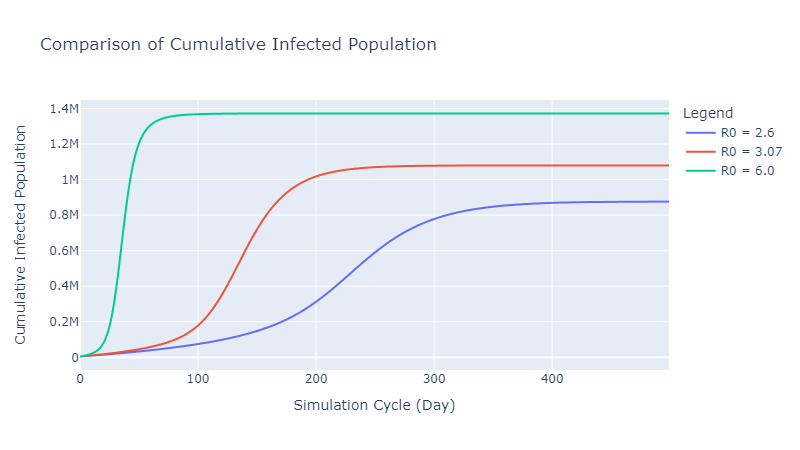
\includegraphics[width=0.95\textwidth]{Figures/InfectedR0.png}
  \caption{Simulations conducted with different basic reproduction ratios ($R_0$). The x-axis represents the simulation cycle (i.e., day), while the y-axis represents the cumulative infected population up to that point in the simulation.} 
  \label{fig:cumulative_infected}
\end{figure}
%python .\infection_sum_comparison.py --p infection_tests --e R0-2.6 R0-3.07 R0-6.0 --l "R0 = 2.6" "R0 = 3.07" "R0 = 6.0" --s 0 --x "Simulation Cycle (Day)" --y "Cumulative Infected Population"

For the remaining experiments, we will consider a baseline value of $R_0 = 2.6$ for the simulations. Figure~\ref{fig:sir_population_status} displays the total population amount for each possible value of the ``SIR Status" traceable characteristic over time in a simulation with $R_0 = 2.6$. It can be observed that despite reaching a cumulative infected population of 875,962 people (as shown in Figure~\ref{fig:cumulative_infected}), the peak of the infection occurred on day 247, with a total of 81,528 infected individuals at that point.

\begin{figure}[ht]
 \centering
  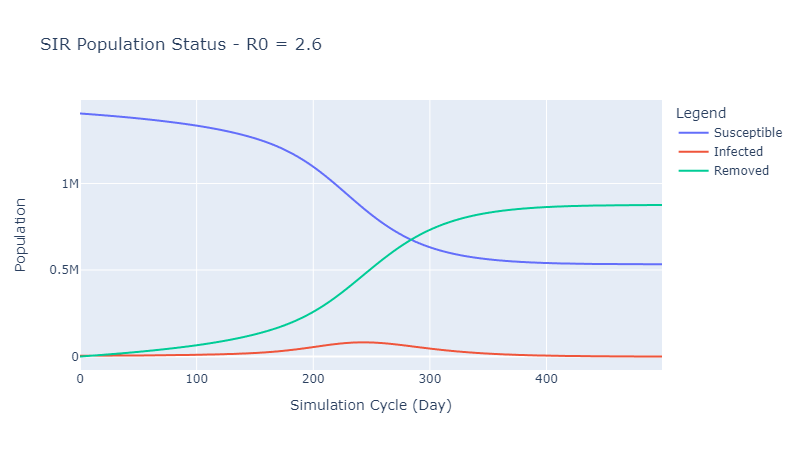
\includegraphics[width=0.95\textwidth]{Figures/SIRPopulationStatus.png}
  \caption{ Population count over time for each ``SIR Status" traceable property value in a simulation with $R_0 = 2.6$} 
  \label{fig:sir_population_status}
\end{figure}
%python .\experiment_global_population.py --p infection_tests --e R0-2.6 --c Susceptible Infected Removed --s 0 --x "Simulation Cycle (Day)" --t "SIR Population Status - R0 = 2.6"



\subsection{Vaccination and Movement Restrictions}
Next, we extend the simulation to include additional behaviors related to epidemic contagion, specifically population vaccination as a measure to mitigate the spread of the disease. To facilitate this, we introduce a traceable characteristic called \textit{vaccine level} to all blobs in the simulation. This property is represented by an integer value. Additionally, we implement a new action called \textit{vaccinate}. When this action is triggered, a portion of the population is moved to a nearby ``pharmacy" $P$, which is available in all regions of the environment. At the pharmacies, the population receives a dose of the vaccine, resulting in an increase of their \textit{vaccine level} by 1. This signifies that they have been vaccinated and their resistance to the transmission of the virus has improved. Subsequently, the newly vaccinated population returns to their respective $P$s, such as workers returning to their ``work" $P$.

In our simulations, we explore various vaccination configurations by considering different dose counts, which represent the number of doses available to the population, as well as the effectiveness of each dose. Table~\ref{tbl:vaccine_configuration} summarizes the vaccination settings used in our experiments, where the Dose Count ranges from 1 to 3. The Effectiveness parameter indicates the efficacy of each dose in mitigating the spread of the infection.

All blobs in simulations with vaccinations contain a \textit{vaccine level} corresponding to an Effectiveness value in Table~\ref{tbl:vaccine_configuration}. Whenever a blob with \textit{SIR Status = Susceptible} gets infected, the amount of people that should be infected is defined by Equation~\ref{eq:deltaI}. The Effectiveness works by multiplying the result of Equation~\ref{eq:deltaI} by $1-Effectivess$, i.e., an $Effectivess=0.4$ reduces the amount of people changing from ``Susceptible" to ``Infected" by $40\%$. Starting Day indicates the simulation cycle at which each dose begins to be administered to the population. It is important to note that the second and third doses, if available, can only be administered to individuals who have already received the previous dose. Configurations A through C represent increasing effectiveness as more doses are administered, while Configuration D represents an ideal vaccine with 100\% effectiveness in preventing infection.

Building upon the parameters defined in previous experiments, all vaccination experiments utilize the routines of workers and students as the baseline, employing a scale parameter of $levy\_scale = 2$ and an \textit{infect} action with $R_0 = 2.6$. The global routine $GRo$ also includes the \textit{vaccinate} action, performed at selected cycle steps during the morning and afternoon of each day. To determine the number of individuals to be moved to ``pharmacy" $P$s on each simulation day, we gathered data on the daily number of COVID-19 vaccines administered in Porto Alegre\footnote{Dashboard of Brazilian vaccination data available \href{https://vacina.saude.rs.gov.br/}{HERE} (text in Brazilian Portuguese)}. This data is then proportionally distributed among the regions in the environment based on their respective populations.

\begin{table}[ht]
\centering
\caption{Configuration of vaccines for experiments. Dose Count represents the number of doses available for the population. Effectiveness represents how effective each dose is in reducing the spread of the infection. Starting Day represents the day (i.e., simulation cycle) when each dose starts being administered to the population. The second and third doses can only be applied to people who already received the previous dose. While VaccinationA, B, and C state for the doses, VaccinationD simulates a scenario where the effectiveness of the vaccine is 100\%.}
\label{tbl:vaccine_configuration}
\begin{tabular}{@{}lccc@{}}
\toprule
Vaccination Config & \multicolumn{1}{l}{Dose Count} & Effectiveness  & Starting Day  \\ \midrule
VaccinationA       & 1                              & {[}0.4{]}           & {[}50{]}           \\
VaccinationB       & 2                              & {[}0.4, 0.7{]}      & {[}50, 150{]}      \\
VaccinationC       & 3                              & {[}0.4, 0.7, 1.0{]} & {[}50, 150, 250{]} \\
VaccinationD       & 1                              & {[}1.0{]}           & {[}50{]}           \\ \bottomrule
\end{tabular}
\end{table}

Figure~\ref{fig:vaccines} showcases the results of the vaccination simulations. Despite the ``VaccinationA" configuration having an effectiveness of only 0.4, a significant impact on the cumulative infected population can be observed compared to the baseline. The baseline simulation resulted in a total of 875,962 infected individuals, whereas the ``VaccinationA" configuration achieved a notably lower count of 440,569 infected individuals. The incorporation of additional doses in the ``VaccinationB" and ``VaccinationC" configurations further decreased the cumulative infected population, resulting in 360,607 and 355,124 infected individuals, respectively. 
Although ``VaccinationC'' contains an effectiveness of $1.0$, this efficacy is only realized when the population undergoes the third dosage, initiated on day 250 of the simulation. Consequently, ``VaccinationB'' and ``VaccinationC'' are very similar until day 250, at which point the third dosage of ``VaccinationC'' begins to exert its influence, resulting in a small difference in the cumulative infected population of both simulations.
\red{Notably, the ``VaccinationD" configuration, representing an ideal vaccine, demonstrates the lowest number of infections, with only 170,978 individuals affected.}

\begin{figure}[ht]
 \centering
  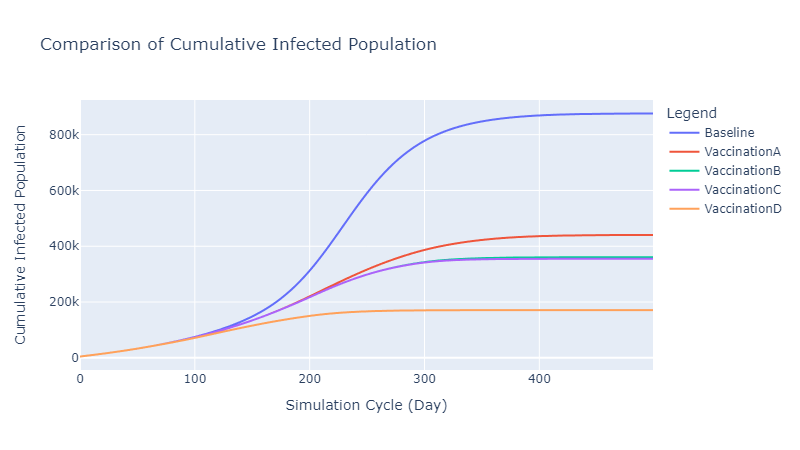
\includegraphics[width=0.95\textwidth]{Figures/InfectedVaccines.png}
  \caption{Simulations of different vaccination configurations, as described in Table~\ref{tbl:vaccine_configuration}. All simulations consider a basic reproduction rate of $R_0 = 2.6$.} 
  \label{fig:vaccines}
\end{figure}

\red{Finally, we explore the incorporation of movement restrictions in our epidemic contagion experiments to simulate lockdown behavior. The movement restriction is described in Section~\ref{sec:random_walk} and illustrated in Figure~\ref{fig7:movement_restriction}.} 
These experiments encompass a combination of three movement restriction values (no restriction, 0.5, and 0.75) that represent percentages of the population who do not leave their living neighborhoods, along with two vaccination scenarios: no vaccination; or ``VaccinationC", which includes three doses. 
We chose to compare the ``VaccinationC'' configuration rather than ``VaccinationD'' because ``VaccinationC'' exhibits a more realistic behavior. In ``VaccinationC'', the effectiveness of the vaccine increases with the number of doses a person receives. In contrast, ``VaccinationD'' represents an idealized vaccine with a fixed effectiveness of $1.0$ achieved in a single dose.

Figure~\ref{fig:vaccines_restrictions} illustrates the results obtained from our simulations. The imposition of movement restrictions reduces the cumulative infected population compared to the baseline scenario (no restriction and no vaccination). However, including population vaccination (experiment ``VaccC") exhibits more significant effectiveness in reducing the infected population compared to simulations with only movement restrictions. Moreover, the combination of movement restriction and vaccination demonstrates the most favorable outcomes, with the simulation containing a movement restriction of 0.75 and vaccination resulting in only 140,941 infected individuals.

%SO: an fig abaixo eu acharia legal comparar com vacin D que tu disseste antes que doi ideal
%GA: no caso trocar C por D ou também incluir D? Posso adicionar mas preciso pegar os resultados no lab, arquivos muito grandes pro git
\begin{figure}[ht]
 \centering
  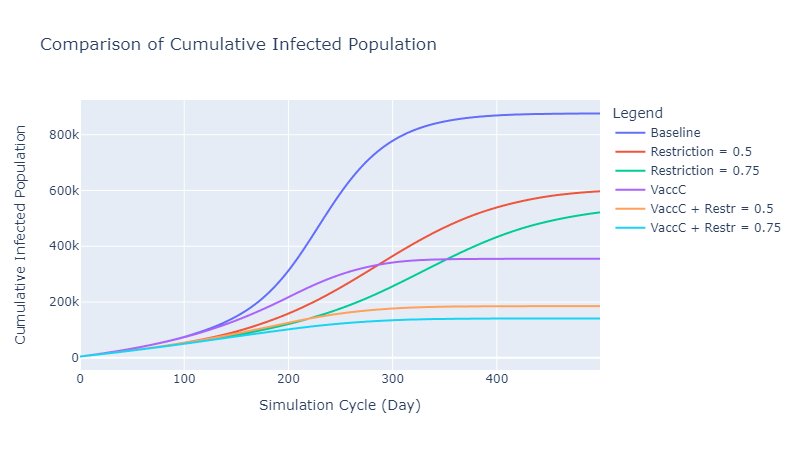
\includegraphics[width=0.95\textwidth]{Figures/InfectedVaccineRestriction.png}
  \caption{ Simulations of epidemic contagion. Experiments include a combination of three movement restriction values (no restriction, 0.5 and 0.75) to represent a lockdown and two vaccination scenarios (no vaccination or ``VaccinationC"). All simulations consider a basic reproduction rate of $R_0 = 2.6$.} 
  \label{fig:vaccines_restrictions}
\end{figure}




\subsection{Intervention Synthesis}

Large events produce temporary concentration and competition for the population available at a particular step. Epidemic contagion instead produces persistent changes in traceable state across hundreds of cycles, and vaccination or movement restrictions alter subsequent transitions and mobility. The studies jointly demonstrate extensibility of demand and population state, but their outputs remain results of the published scenario assumptions rather than calibrated forecasts.

\section{Environmental Disruption and Destination Adaptation}
\label{sec:flood_mobility}

\subsection{Modeling Flood Exposure}

The flood experiments apply time-indexed water levels and node exposure attributes to the effective-availability mechanism in Section~\ref{sec:proposed_model}. A flood cause can disable homes, activity points of interest, workplaces, or schools. Availability alone does not prescribe a response: the consuming plugin may suppress demand, record an unavailable origin or destination, delay a return, or select an explicit fallback.

\subsection{Popular Times Flood Matrix}
The Stage 4 matrix contains 130 runs over 56 simulated days. Levy-off configurations are deterministic and run once. The 13-region Levy-on configurations use matched seeds 0--29, and the 94-region Levy-on no-flood configuration uses five seeds. All runs pass population-conservation and enabled-node movement checks.

Flooding activity destinations suppresses 83,445 requested visits, reducing fulfillment from 100\% to 96.49\%. Flooding homes alone maintains complete visit fulfillment but increases sourcing distance because travelers must be drawn from other enabled homes. Enabling legacy Levy movement changes sourcing distance but not the amount of requested activity fulfilled. Table~\ref{tbl:popular_core} reports the principal 13-region Levy-on conditions. The 94-region comparison is limited to the no-flood baseline and also achieves complete fulfillment.

\begin{table}[ht]
\centering
\footnotesize
\caption{Stage 4 13-region Levy-on outcomes over 30 matched seeds.}
\label{tbl:popular_core}
\begin{tabularx}{\linewidth}{@{}lrrrX@{}}
\toprule
\textbf{Flood exposure} & \textbf{Fulfillment} & \textbf{Travelers/capita} & \textbf{Distance/request} & \textbf{Interpretation} \\ \midrule
None & 1.0000 & 17.9997 & 81.9953 & Reference \\ 
POIs & 0.9649 & 17.3672 & 76.2669 & Destination demand suppressed \\ 
Homes & 1.0000 & 17.9997 & 88.9408 & Full demand sourced farther away \\ 
Homes and POIs & 0.9649 & 17.3672 & 76.8287 & POI loss determines fulfillment \\ \bottomrule
\end{tabularx}
\end{table}



\subsection{Activity-Destination Adaptation}
Stage 5 evaluates nearest-enabled, same-type POI substitution for the combined home-and-POI flood condition. The deterministic Levy-off run and 30 matched Levy-on runs all pass their invariants. In every run, all 83,445 visits previously suppressed by a disabled destination are rerouted, restoring fulfillment from 96.49\% to 100\%. Mean additional POI displacement is 297.89~m per rerouted traveler, and the maximum receiving load is 92 travelers. These values measure the cost and concentration produced by the implemented nearest-safe policy; they do not demonstrate that residents would select the same alternatives in practice.



\subsection{Flood-Aware Commuting Model}
Levy Walk V2 replaces opportunistic legacy movement with explicit worker and student attendance. Cycle-level targets are allocated exactly across homes and hourly departure profiles. Trips are divided into packets of no more than 50 people. The plugin audits demand suppressed at disabled origins, unavailable or imminently flooded destinations, temporary return homes, blocked returns, and later repatriation.



\subsection{Stage 6 Disruption Results}
Stage 6 contains five 13-region families with seeds 0--29 and 56 simulated days. All 150 runs pass both the Popular Times and Levy Walk V2 validations. Table~\ref{tbl:levy_v2} shows that commute fulfillment falls under each flood mode and is lowest when all node types are exposed. Popular Times rerouting restores activity visits in the combined condition but does not restore work and school attendance.

\begin{table}[ht]
\centering
\footnotesize
\caption{Stage 6 outcomes over 30 matched seeds; brackets contain 95\% intervals.}
\label{tbl:levy_v2}
\begin{tabularx}{\linewidth}{@{}lXXX@{}}
\toprule
\textbf{Scenario} & \textbf{Commute fulfillment} & \textbf{Mean commute distance (m)} & \textbf{Activity fulfillment} \\ \midrule
No flood & 1.0000 [1.0000--1.0000] & 1,393.53 [1,392.87--1,394.19] & 1.0000 \\ 
Destinations flooded & 0.9354 [0.9352--0.9355] & 1,343.80 [1,343.03--1,344.56] & 0.9649 \\ 
Homes flooded & 0.9406 [0.9404--0.9408] & 1,390.89 [1,390.10--1,391.69] & 1.0000 \\ 
All node types flooded & 0.8915 [0.8912--0.8917] & 1,335.82 [1,335.02--1,336.62] & 0.9649 \\ 
All flooded, POIs rerouted & 0.8905 [0.8903--0.8908] & 1,335.82 [1,334.98--1,336.67] & 1.0000 \\ \bottomrule
\end{tabularx}
\end{table}

Cross-version results are labeled combined model revisions. Levy Walk V2 changes commute demand and lifecycle semantics, and destination flooding now includes work and school. Similarity in the shared Popular Times metrics therefore checks compatibility, but differences do not isolate an algorithmic improvement over the legacy Levy action.



\subsection{Disruption and Adaptation Synthesis}
The three stages separate disruption from response. Stage 4 quantifies unmet demand when unavailable destinations are simply suppressed. Stage 5 adds an explicit substitution rule and measures its travel and receiving-load consequences. Stage 6 shows that the same rule can restore activity visits while assigned work and school trips remain disrupted. The broader result is not that one category is intrinsically discretionary, but that substitutability must be represented explicitly for each destination type. A model that silently replaces all unavailable destinations would hide this assumption and overstate adaptation.



\section{Health and Critical-Service Resilience}
\label{sec:health_resilience}

\subsection{From Population Health to Service Access}

The epidemic experiments in Section~\ref{sec:interventions} model population state and transmission. The studies in this chapter instead model access to scarce services. Inpatient and dialysis plugins introduce capacity, admission, waiting, recurring demand, failure, and recovery policies without promoting them to universal properties of every point of interest. The three health-related families therefore demonstrate complementary framework capabilities, but their infection and service-access metrics are not directly comparable.

\subsection{LODUS-Health Lineage}
LODUS-Health introduced a Porto Alegre hospital dataset, a configurable bed-occupancy simulation, a web interface, and medical-text generation~\citep{souza2026lodushealth}. It provides the conceptual and data basis for the recent inpatient work. The present evaluation does not merge its original figures or simulation outcomes with the new batch. Instead, the January 2024 capacity source and the idea of moving cohorts from homes to hospitals are carried forward into a new plugin with explicit payer pools, lengths of stay, overflow and queue policies, and auditable demand records.

The dialysis study uses the same general pattern---population demand traveling from homes to geographically located services---but introduces recurring treatment, clinic schedules, admission capacity, recovery, flooding, and infrastructure dependencies. The two studies therefore test related access questions while retaining distinct service semantics and metrics.



\subsection{Inpatient-Care Model and Scenario Design}
Inpatient demand is represented by cohorts sharing an origin, diagnosis or specialty category, payer, preferred destination, and length of stay. Each hospital exposes separate SUS and private capacity pools. Discharges release capacity after the configured stay. A disabled preferred hospital may be replaced by an enabled configured fallback, but the experiments do not assume unconstrained dynamic load balancing.

The \textit{overflow} policy admits all eligible demand and records occupancy beyond the configured bed count. It is a counterfactual for measuring latent shortage, not an operational policy. The \textit{queue} policy enforces capacity and retains unserved cohorts in a first-in, first-out queue. Seven scenarios cover reference and high demand under both policies, a fixed two-facility allocation under both policies, and a small queue-based CID-routing demonstration. Each scenario uses seeds 0--29.



\subsection{Inpatient-Care Results}
Table~\ref{tbl:inpatient_results} reports the batch summary. Reference demand is almost fully served under the queue policy. Under high demand, unconstrained overflow reveals an average peak excess of 333.8 patients, while enforcing capacity reduces mean coverage to 52.10\% and leaves an average final queue of 1,336.5. The fixed two-facility configuration raises queue-policy coverage to 97.08\% and reduces the final queue to 77.2 patients. The CID demonstration achieves 96.13\% mean coverage and a population-weighted mean admission distance of 3.16~km.

\begin{table}[ht]
\centering
\footnotesize
\caption{Inpatient-care outcomes over 30 seeds. Intervals are the reported P05--P95 ranges.}
\label{tbl:inpatient_results}
\begin{tabularx}{\linewidth}{@{}lXXXX@{}}
\toprule
\textbf{Scenario} & \textbf{Coverage} & \textbf{Peak overflow} & \textbf{Final queue} & \textbf{Mean delay} \\ \midrule
Reference overflow & 1.0000 [1.0000--1.0000] & 0.4 [0.0--2.5] & 0.0 & 0.00 \\ 
Reference queue & 0.9996 [0.9972--1.0000] & 0.0 & 0.2 [0.0--1.5] & 0.00 \\ 
High-demand overflow & 1.0000 [1.0000--1.0000] & 333.8 [320.4--349.1] & 0.0 & 0.00 \\ 
High-demand queue & 0.5210 [0.5105--0.5297] & 0.0 & 1,336.5 [1,312.0--1,365.8] & 2.44 [2.34--2.56] \\ 
Two-facility overflow & 1.0000 [1.0000--1.0000] & 52.5 [37.5--70.0] & 0.0 & 0.00 \\ 
Two-facility queue & 0.9708 [0.9570--0.9809] & 0.0 & 77.2 [50.5--113.5] & 0.14 [0.09--0.21] \\ 
CID-routing queue & 0.9613 [0.9151--1.0000] & 0.0 & 8.7 [0.0--19.1] & 1.14 [1.02--1.26] \\ \bottomrule
\end{tabularx}
\end{table}

The two-facility result demonstrates the consequence of a configured spatial allocation, not an inferred optimal policy. Santa Ana's psychiatric capacity is synthetic. The CID demand and mappings are also synthetic, and the six-origin demonstration is too small to support clinical conclusions. Patients admitted or waiting at the final step are horizon-censored, and the original per-step distributions from the earlier dissertation experiments were not retained; exact reproduction of those earlier timings is therefore outside the scope of this batch.



\subsection{Dialysis-Service Model and Scenario Design}
The dialysis plugin creates patients with recurring treatment demand every three days, assigns them to home nodes, and admits due patients to enabled clinics subject to schedules and per-step capacity. Unserved patients remain due, allowing treatment coverage, waiting exposure, and overdue demand to be measured. Admission events retain the home origin, receiving clinic, and distance.

The K00--K11 catalog compares a reduced 13-region service network with a complete-city network. Conditions include reference and moderate demand, above-capacity demand, a persistent outage, rapid recovery after four hours, a historical clinic-flood pattern, a synthetic water-treatment failure, combined disruptions, and two failure topologies with matched aggregate capacity loss. Disruptions begin on the third simulated day, and the primary comparisons use matched seeds 0--29.



\subsection{Dialysis-Service Results}
Reference and moderate-demand scenarios K00, K01, and K10 complete every due treatment. Above-capacity K07 attains 93.02\% coverage despite no facility outage. The persistent Moinhos outage in K02 reduces coverage to 68.52\%, whereas four-hour recovery in K03 restores 100\% coverage. The historical clinic-flood condition K04 also maintains complete coverage through available alternatives.

The synthetic water-treatment failure in K05 and the combined reduced-network disruption in K06 each reduce coverage to 50\%. In the complete network, the corresponding combined disruption K11 maintains 71.43\% coverage. Thus, a larger network improves the modeled outcome but does not eliminate the effect of widespread dependent failures.

Failure topology changes travel even when coverage and nominal lost capacity are similar. K08 removes one high-capacity clinic and K09 removes several lower-capacity clinics; both maintain complete coverage, but mean admission distance rises from 1.768~km in K08 to 2.037~km in K09. The comparison indicates that aggregate capacity alone does not characterize the spatial burden imposed by a disruption.

\begin{table}[ht]
\centering
\footnotesize
\caption{Mean dialysis outcomes. Each scenario has 30 primary seeds; K03 retains one additional completed record.}
\label{tbl:dialysis_results}
\begin{tabularx}{\linewidth}{@{}llrrX@{}}
\toprule
\textbf{ID} & \textbf{Condition} & \textbf{Coverage} & \textbf{Distance (km)} & \textbf{Interpretive role} \\ \midrule
K00 & Reduced reference & 1.0000 & 1.716 & Reference demand \\ 
K01 & Reduced moderate & 1.0000 & 1.836 & Disruption control \\ 
K02 & Persistent Moinhos outage & 0.6852 & 2.090 & Persistent isolated failure \\ 
K03 & Four-hour recovery & 1.0000 & 1.833 & Recovery contrast \\ 
K04 & Historical clinic flood & 1.0000 & 1.768 & Clinic exposure \\ 
K05 & Synthetic water failure & 0.5000 & 1.845 & Cascading dependency \\ 
K06 & Combined reduced failure & 0.5000 & 1.845 & Compound disruption \\ 
K07 & Reduced above capacity & 0.9302 & 1.854 & Demand stress \\ 
K08 & One high-capacity failure & 1.0000 & 1.768 & Concentrated topology \\ 
K09 & Matched small failures & 1.0000 & 2.037 & Distributed topology \\ 
K10 & Complete moderate & 1.0000 & 6.537 & Complete-network control \\ 
K11 & Complete combined & 0.7143 & 7.052 & Complete-network disruption \\ \bottomrule
\end{tabularx}
\end{table}



\subsection{Health-Service Synthesis}
The two health studies expose complementary aspects of access. Inpatient care shows the difference between latent shortage and an enforced queue, and it shows how a configured distribution of demand across facilities can change coverage and delay. Dialysis shows how recurring service, recovery time, failure topology, and supporting infrastructure affect treatment completion and travel. Across both, total capacity is necessary but insufficient: where capacity is located, whether it is available, and how demand is routed determine the modeled burden. Coverage, overflow, queues, overdue treatments, and distance remain domain-specific measures and are not collapsed into a single resilience score.



\section{Computational and Analytical Support}
\label{sec:computational_analysis}
\label{sec:visualization}

\subsection{Scope of the Computational Evaluation}

The computational measurements reproduced below cover the original random-walk, large-event, epidemic, and vaccination configurations. They characterize those published runs on one machine; they are not presented as benchmarks for every recent experiment or as head-to-head comparisons with another simulator.

\subsection{Published Runtime and Memory Results}
\label{sec:quant_perf}

\redc{To complement the qualitative case studies, we present a quantitative evaluation of LodusPop’s computational efficiency. All benchmarks use the Porto Alegre city model described in Section~\ref{sec:case_scenario} (94 regions, 504 points of interest, and a total population of $1,409,351$). Each configuration was executed five times, and average values are reported.

Table~\ref{tab:perf} reports quantitative information for each \textit{Case Study} and \textit{Configuration}, as follows: (i) \textit{Max Blob Count}, the maximum number of blobs observed during the run; (ii) \textit{Number of Cycles}, where a cycle corresponds to one simulated day in our setup, with 24 cycle steps; (iii) \textit{Avg Sim Time (s)}, the average total real-time required to complete the run; (iv) \textit{Time Per Cycle (s)}, the average runtime per simulated day; (v) \textit{MemProfile Avg Peak (MiB)}, the average peak resident memory of the Python process\footnote{Calculated with Memory Profiler v0.61.0: \url{https://pypi.org/project/memory-profiler/}}; and (vi) \textit{TraceMalloc Avg Peak (MiB)}, the average peak traced Python allocations\footnote{Calculated with TraceMalloc: \url{https://docs.python.org/3/library/tracemalloc.html}}. We interpret \textit{Max Blob Count} as an indicator of simulator workload: more frequent splits increase the number of population units to process and reduce merge opportunities, typically raising both runtime and memory consumption.

Using the random walk configuration of $levy\_scale=2$ (Section~\ref{sec:random_walk}) as the baseline simulation for the remaining case studies and configurations, the simulator completes a full run in $5.211s$ on average, with \emph{MemProfile Avg Peak} of $234.9$~MiB, and a \textit{TraceMalloc Avg Peak} of $58.565$~MiB. Introducing movement restrictions (Section~\ref{sec:random_walk}) slightly reduces \textit{Time Per Cycle} (down to $4.795s$ at $Restriction =0.75$), while peak memory remains essentially unchanged. This indicates that reduced mobility mainly decreases the number of executed move operations, without substantially changing blob splitting, as expected.

Large-scale events (Section~\ref{sec:large_scale}) increase runtime because they introduce additional gathering actions that relocate populations across distant locations. \textit{Time Per Cycle} rises from $6.144s$ (average simulations with one event) to $12.172s$ (simulation with four simultaneous events). These scenarios tend to produce fewer blobs, as populations aggregate around event locations, yet \textit{MemProfile Avg Peak} and \textit{TraceMalloc Avg Peak} remain close to the baseline ($\approx 235$~MiB and $\approx 59$~MiB, respectively). This indicates that the dominant cost comes from executing the large-scale gathering operations by pulling individuals from multiple regions and points of interest, rather than from an increase in blob count.

Epidemic contagion and vaccination simulations (Section~\ref{sec:contagion}) are more demanding because additional traceable characteristics (e.g., SIR status and vaccine level) increase population heterogeneity, causing more frequent splits and reducing merge opportunities. In our model, blobs can only merge when their traceable attributes match; as the simulation progresses, individuals become distributed across multiple states (susceptible, infected, removed) and vaccination levels, so blobs with different traceable characteristics cannot be merged back together.
For infection-only experiments, 500-cycle runs require $9.899$--$11.654s$ per cycle, and \textit{MemProfile Avg Peak} increases to roughly $1.72$--$1.80$~GiB. Vaccination scenarios further intensify splitting: VaccinationC reaches a \textit{Max Blob Count} of $23,355$ and requires $33.455s$ per cycle, with \textit{MemProfile Avg Peak} of $2.86$~GiB. Overall, \textit{Time Per Cycle} closely follows increases in \textit{Max Blob Count}, reinforcing that split and merge behaviors are key components of computational cost.

%Limitações das medidas
These measurements reflect the simulator execution on a single machine and are therefore hardware-dependent. The results are intended as a quantitative evaluation of the presented case studies, providing direct support for the efficiency and scalability claims within their scope, rather than as a head-to-head comparison with other simulation frameworks. 
All experiments were run on a machine with an AMD Ryzen 5 5600X CPU, an NVIDIA GeForce RTX 2060 GPU, 16GB DDR4 2666MHz (CL19) RAM, and a KINGSTON SNV3S1000G SSD, using Python v3.13.6 on Microsoft Windows 11 Education (Version 10.0.262000).}

\begin{table}[ht]
\redc{
\footnotesize
\centering
\caption{\redc{Quantitative performance evaluation of LodusPop. We use the Random Walk mobility configuration (Lévy-flight simulation with $levy\_scale=2$; Section~\ref{sec:random_walk}) as the baseline reference for the remaining case studies and configurations. For each case study and configuration, we report the maximum blob count observed during execution, the number of simulated cycles (days), the average total simulation time over five runs, the corresponding time per cycle, and peak memory usage measured via MemProfile (process RSS) and TraceMalloc (Python allocation tracing).}}
\label{tab:perf}
\begin{tabular}{@{}clllllll@{}}
\toprule
Case Study                                                                                                               & \multicolumn{1}{c}{Configuration} & \multicolumn{1}{c}{\begin{tabular}[c]{@{}c@{}}Max Blob\\ Count\end{tabular}} & \multicolumn{1}{c}{\begin{tabular}[c]{@{}c@{}}Number\\ of Cycles\end{tabular}} & \multicolumn{1}{c}{\begin{tabular}[c]{@{}c@{}}Avg Sim\\ Time (s)\end{tabular}} & \multicolumn{1}{c}{\begin{tabular}[c]{@{}c@{}}Time Per\\ Cycle (s)\end{tabular}} & \multicolumn{1}{c}{\begin{tabular}[c]{@{}c@{}}MemProfile\\ Avg Peak\\ (MiB)\end{tabular}} & \multicolumn{1}{c}{\begin{tabular}[c]{@{}c@{}}TraceMalloc\\ Avg Peak\\ (MiB)\end{tabular}} \\ \midrule
\begin{tabular}[c]{@{}c@{}}Baseline\\ (Random Walk)\\Case Study 1\end{tabular}                                                                                                                & $levy\_scale = 2$                          & 2857                                                                         & 1                                                                              & 5.211                                                                          & 5.211                                                                            & 234.912                                                                                 & 58.565                                                                                   \\ \midrule
\multirow{3}{*}{\begin{tabular}[c]{@{}c@{}}Movement \\Restriction (Fig~\ref{fig7:movement_restriction})\\Case Study 1\end{tabular}}                                         & Restriction = 0.25                & 2871                                                                         & 1                                                                              & 5.074                                                                          & 5.074                                                                            & 234.957                                                                                 & 58.577                                                                                   \\
                                                                                                                       & Restriction = 0.50                & 2864                                                                         & 1                                                                              & 4.958                                                                          & 4.958                                                                            & 234.935                                                                                 & 58.527                                                                                   \\
                                                                                                                       & Restriction = 0.75                & 2883                                                                         & 1                                                                              & 4.795                                                                          & 4.795                                                                            & 235.234                                                                                 & 58.516                                                                                   \\ \midrule
\multirow{5}{*}{\begin{tabular}[c]{@{}c@{}}Large-Scale Events\\ (Fig~\ref{fig8:results_displacements} and Table~\ref{tbl:results_displacement})\\Case Study 2\end{tabular}}                                 & Average of 1 Event                & 2671                                                                         & 1                                                                              & 6.144                                                                          & 6.144                                                                            & 235.355                                                                                 & 58.767                                                                                   \\
                                                                                                                       & Average of 2 Events               & 2651                                                                         & 1                                                                              & 7.986                                                                          & 7.986                                                                            & 235.297                                                                                 & 58.892                                                                                   \\
                                                                                                                       & Average of 3 Events               & 2651                                                                         & 1                                                                              & 9.910                                                                          & 9.910                                                                            & 235.530                                                                                 & 59.061                                                                                   \\
                                                                                                                       & 4 Events                          & 2651                                                                         & 1                                                                              & 12.172                                                                         & 12.172                                                                           & 235.825                                                                                 & 59.217                                                                                   \\
                                                                                                                       & 4 Events at Different Times       & 2079                                                                         & 1                                                                              & 11.153                                                                         & 11.153                                                                           & 235.355                                                                                 & 59.146                                                                                   \\ \midrule
\multirow{3}{*}{\begin{tabular}[c]{@{}c@{}}Infection (Fig~\ref{fig:cumulative_infected})\\Case Study 3\end{tabular}}                                          & $R_0$ = 2.6                          & 8840                                                                         & 500                                                                            & 5826.840                                                                       & 11.654                                                                           & 1798.114                                                                                & 1554.886                                                                                 \\
                                                                                                                       & $R_0$ = 3.07                         & 8830                                                                         & 500                                                                            & 5630.155                                                                       & 11.260                                                                           & 1741.606                                                                                & 1520.793                                                                                 \\
                                                                                                                       & $R_0$ = 6.0                          & 8818                                                                         & 500                                                                            & 4949.313                                                                       & 9.899                                                                            & 1718.252                                                                                & 1480.354                                                                                 \\ \midrule
\multirow{4}{*}{\begin{tabular}[c]{@{}c@{}}Vaccination\\ (Fig~\ref{fig:vaccines} and Table~\ref{tbl:vaccine_configuration})\\Case Study 3\end{tabular}}                                        & VaccA                             & 16495                                                                        & 500                                                                            & 8991.828                                                                       & 17.984                                                                           & 2246.849                                                                                & 2057.299                                                                                 \\
                                                                                                                       & VaccB                             & 20840                                                                        & 500                                                                            & 11346.181                                                                      & 22.692                                                                           & 2250.278                                                                                & 2318.228                                                                                 \\
                                                                                                                       & VaccC                             & 23355                                                                        & 500                                                                            & 16727.571                                                                      & 33.455                                                                           & 2862.153                                                                                & 2512.703                                                                                 \\
                                                                                                                       & VaccD                             & 12542                                                                        & 500                                                                            & 7620.026                                                                       & 15.240                                                                           & 1750.923                                                                                & 1883.745                                                                                 \\ \midrule
\multirow{4}{*}{\begin{tabular}[c]{@{}c@{}}Vaccination and\\Restriction (Fig~\ref{fig:vaccines_restrictions})\\Case Study 3\end{tabular}} & $R_0$ = 2.6; Restriction = 0.50      & 9011                                                                         & 500                                                                            & 4008.347                                                                       & 8.017                                                                            & 1983.816                                                                                & 1743.626                                                                                 \\
                                                                                                                       & $R_0$ = 2.6; Restriction = 0.75      & 8320                                                                         & 500                                                                            & 4566.876                                                                       & 9.134                                                                            & 1681.857                                                                                & 1472.081                                                                                 \\
                                                                                                                       & VaccC; Restriction = 0.50         & 16722                                                                        & 500                                                                            & 9279.227                                                                       & 18.558                                                                           & 2628.414                                                                                & 2313.595                                                                                 \\
                                                                                                                       & VaccC; Restriction = 0.75         & 15429                                                                        & 500                                                                            & 8139.657                                                                       & 16.279                                                                           & 2540.851                                                                                & 2240.514                                                                                 \\ \bottomrule
\end{tabular}
} %  end of redc
\end{table}



\subsection{Simulation Outputs and Origin--Destination Flows}
LodusPop records complementary views of a run. Population and node-state logs describe occupancy, characteristics, effective availability, and disable causes over time. Movement records retain origin, destination, step, and moved population. Domain loggers add demand, admission, queue, rerouting, and unmet-reason events. These records can be aggregated into node, region, census-sector, and origin--destination tables without changing the simulated state.

An origin--destination matrix reports how much population moved between two units during a step, cycle, or complete run. It does not encode the route between their representative coordinates. This distinction is important for interpreting both the immersive and geographic-flow tools.



\subsection{Immersive Virtual-Reality Visualization}
Teixeira et al.~\citep{teixeira2024visualization} developed a Unity application for the Meta Quest 2 that loads an OpenStreetMap-derived environment, monitored nodes, and formatted LODUS output. Users can inspect occupancy at the current step or over time, group regions of interest, and view moving healthy and infected populations within a three-dimensional map. Capacity-oriented displays highlight potential overcrowding.

The demonstration used 13 regions of interest, seven steps, and randomly generated displacement and infection events. It therefore evaluates whether the prototype can ingest and present the data format. It does not validate a hospital-demand process, contamination model, or planning intervention. The study itself identifies controlled user studies as future work for usability and analytical effectiveness.



\subsection{Interactive Geographic Flow Visualization}
The student-led geographic flow tool~\citep{silva2026geospatial} uses React, TypeScript, MapLibre, and DuckDB-WASM to query and display origin--destination data in the browser. It supports selection of territorial units, incoming and outgoing flows, density controls, demographic filters, coordinated indicators and charts, multiscale aggregation, reusable configuration profiles, and local caching.

Its principal evaluation uses 2021 England and Wales census commuting at Middle Layer Super Output Area and Lower Tier Local Authority levels. A simulated Porto Alegre dataset tests reuse with another geography. Lines connect territorial centroids and therefore show aggregate relationships rather than traveled paths. The reported latency evaluation is exploratory and does not replace a controlled performance or user study.



\subsection{Application to Recent Experiments}
The recent loggers already produce compatible aggregate relations: home--clinic flows for dialysis, origin--hospital flows for inpatient care, home--POI flows for Popular Times, and home--work or home--school flows for Levy Walk V2. Node-state records can additionally identify when a destination was disabled and why. These interfaces make integration with the geographic-flow tool feasible and allow immersive views to animate formatted transfers.

No completed study in this thesis evaluates those recent batches inside either visualization application. Their compatibility is therefore presented as a supported integration path, not as an experimental result. A future evaluation should define analytical tasks, compare views, recruit intended users, and measure accuracy, time, confidence, and usability.



\subsection{Capabilities, Limitations, and Author Contributions}
Visualization supports inspection, communication, and anomaly discovery. It can reveal concentrated flows, unexpected receivers, overcrowded nodes, and changes over time. It cannot establish that the generating assumptions match observed behavior. Geographic aggregation can conceal within-area variation, centroid lines can imply nonexistent routes, and three-dimensional animation can give synthetic data an unwarranted appearance of realism.

The immersive prototype is collaborative published work by Teixeira, the thesis author, and their coauthors; this thesis does not claim that it was developed solely by the thesis author. The geographic flow application and manuscript were developed by Gustavo Willian Martins da Silva as student-led work under the thesis author's supervision. The present thesis contributes the integration and critical synthesis of these artifacts with the recent LodusPop outputs.



\section{Discussion}
\label{sec:discussion}
\subsection{Answers to the Research Questions}
\label{discussion:questions}

\textbf{RQ1---representation across granularities.} The same region, point-of-interest, blob, template, and action abstractions support both the original neighborhood scenario and the recent census-sector home distributions. Moving from 94 aggregated homes to 435 or 2,711 census-sector homes changes the input graph and possible travel distances, not the population model. The experiments therefore demonstrate representational reuse. They do not establish that every spatial resolution is equally accurate; the appropriate resolution remains constrained by data and the phenomenon being studied.

\textbf{RQ2---extension without changing the core.} Disease states, hospital admissions, recurring dialysis demand, activity visits, commuting, and flood response are implemented by plugins consuming the same population and environment interfaces. Cause-aware availability and dependencies provide the common environmental state needed by several plugins. Capacity, queues, rerouting, and return lifecycles remain domain-specific. This boundary is the principal architectural answer to RQ2.

\textbf{RQ3---versatility and limits.} The original and recent studies cover substantially different timescales, destination types, population selections, and outcome metrics. Their successful execution and invariant checks show that the framework can express these scenarios. The health and flood results also produce interpretable within-model contrasts. Versatility is therefore supported as software and modeling capability; predictive validity is not established across the application domains.

\textbf{RQ4---auditable interpretation.} Explicit provenance, matched seeds, deterministic/stochastic separation, demand accounting, node-state logs, conservation checks, and domain event logs make scenario outcomes traceable. Visualization can help inspect the records, but it is not a substitute for calibration or external validation. The strongest interpretation is thus a reproducible comparison between named configurations.

\subsection{Evidence of Framework Extensibility}

Table~\ref{tbl:cross_study_synthesis} summarizes how the studies reuse the core while changing plugin-level mechanisms. No single metric spans all rows because each experiment represents a different construct. The relevant framework evidence is that populations remain conserved and traceable while the environment and plugins express each domain's demand and response.

\begin{table}[ht]
\centering
\scriptsize
\caption{Cross-study synthesis of framework use, evidence, and limits.}
\label{tbl:cross_study_synthesis}
\begin{tabularx}{\linewidth}{@{}p{2.0cm}p{2.0cm}p{2.5cm}XX@{}}
\toprule
\textbf{Study} & \textbf{Spatial input} & \textbf{Extension or disruption} & \textbf{Response and metrics} & \textbf{Principal limit} \\ \midrule
Original cases & 94 neighborhood homes & Levy movement, events, contagion, vaccination & Movement, infection, blob count, runtime, memory & Aggregated homes and no dynamic facility loss \\ \midrule
Inpatient care & 94 regions; census-sector homes & Bed pools, stays, disabled facilities, demand stress & Overflow or FIFO queue; coverage, delay, distance & Synthetic demand elements and horizon censoring \\ \midrule
Dialysis & Reduced and complete census-sector environments & Recurring demand, outages, recovery, water dependencies & Admission to enabled capacity; coverage, overdue demand, distance & Configured demand and disruption schedules \\ \midrule
Popular Times & 13-region flood matrix; 94-region no-flood baseline & Weekly visits, flooded homes and POIs & Suppression or nearest-safe rerouting; fulfillment and displacement & Fixed profiles and unvalidated substitution behavior \\ \midrule
Levy Walk V2 & 13 regions; census-sector homes & Work/school attendance and flood-aware returns & Commute fulfillment, unmet reasons, distance, repatriation & Assigned destinations and combined cross-version changes \\ \midrule
Visualization & Node, temporal, and OD outputs & Immersive and multiscale geographic views & Exploration of occupancy and flows & Synthetic/exploratory evaluations, not validation \\ \bottomrule
\end{tabularx}
\end{table}

The plugin architecture also prevents successful behavior in one domain from silently becoming a general rule. The nearest-safe policy restores Popular Times visits, but it is not applied to dialysis, hospital admissions, workplaces, or schools unless a corresponding plugin explicitly defines that policy. This makes model composition more verbose, but it preserves the assumptions needed to audit a result.

\subsection{Spatial Resolution and Data Availability}
\label{discussion:spatial}

The meaning of a region and point of interest is selected by the simulation designer. A point may represent a specific building, all facilities of a type in a neighborhood, or an abstract location at a broader scale. Distances and domain parameters must be interpreted consistently with that choice. A contagion parameter calibrated for building-scale contact, for example, cannot be transferred unchanged to movement between cities or states.

The recent census-sector environments make the flexibility discussed in the original manuscript concrete. Multiple home nodes now occur within one neighborhood, allowing sources and flood exposure to vary within the region. This improves spatial expression but increases input size and does not automatically improve behavioral validity. Census and municipal datasets may be outdated or incomplete, and sampled characteristics may omit joint dependencies between age, occupation, payer, and mobility. Resolution should therefore be justified by the research question and source data rather than maximized as an end in itself.

\subsection{Capacity, Failure Topology, Dependencies, and Adaptation}

The health experiments show that availability and capacity answer different questions. The inpatient overflow policy reveals latent shortage, while the queue policy represents the consequence of enforcing capacity. Dialysis failures show that nominal capacity loss can be temporary, persistent, concentrated, distributed, or caused indirectly through a dependency. Coverage alone is insufficient: two conditions with complete treatment coverage can impose different travel burdens.

The mobility experiments likewise separate exposure and response. Disabling a destination suppresses demand under one policy and invokes substitution under another. Restoring activity-visit fulfillment adds displacement and receiving load and does not repair assigned work or school trips. These results favor reporting a vector of outcomes---coverage or fulfillment, delay or unmet demand, travel, and load---over a single composite resilience score whose weights would introduce additional assumptions.

\subsection{Visualization as Interpretation Rather Than Validation}

Immersive and geographic visualizations expose temporal occupancy and spatial flows that are difficult to interpret in raw tables. They are especially relevant for investigating redistributed clinic demand, hospital catchments, replacement POIs, and commute disruptions. However, a coherent animation or map shows that records can be rendered, not that the generating process is realistic. Validation requires an independent observed quantity and a defined comparison criterion. The synthetic VR demonstration and exploratory OD-tool evaluation are therefore presented as supporting capabilities.

\subsection{Threats to Validity and Reproducibility}
\label{discussion:validity}

\textbf{Construct validity.} Coverage, fulfillment, overflow, queue length, and distance approximate different dimensions of service or mobility. They do not measure welfare, clinical outcome, equity, or individual preference. Fixed visit profiles and assigned destinations simplify adaptive behavior.

\textbf{Internal validity.} Automated invariants and matched scenarios reduce implementation and comparison errors, but they cannot prove the absence of defects. Several outcomes are deterministic consequences of fixed demand and node schedules. Confidence intervals over seeds quantify only the stochastic components of the implementation.

\textbf{External validity.} Facility and geographic data anchor the scenarios in Porto Alegre, but many demand values, thresholds, failures, mappings, and alternatives are configured or synthetic. The results should not be extrapolated as forecasts. In particular, Santa Ana capacity, CID demand, and CID mappings are demonstrations, and the nearest-safe POI rule has not been compared with observed post-disruption choices.

\textbf{Statistical validity.} The batches use different summaries appropriate to their preserved reports: inpatient results provide P05--P95 ranges, dialysis analysis uses bootstrap intervals, and the repeated mobility studies use reported 95\% $t$ intervals. Deterministic conditions are not assigned artificial intervals. Cross-domain metrics are not pooled, and the Stage 6 legacy comparison is not interpreted as an isolated algorithm effect.

\textbf{Reproducibility.} Recent configurations, raw outputs, run metadata, summaries, and validation artifacts are retained in the repository. The older LODUS-Health per-step distributions and seed were not retained, so its exact published timing is not reproducible; the new inpatient batch is the reproducible evidence used here. Software and data versions should be archived with the final thesis.

\subsection{Future Work}

The highest-priority methodological work is calibration against observed mobility and health-service data, sensitivity analysis for demand and flood thresholds, joint rather than independent population-characteristic distributions, and explicit uncertainty in external inputs. Health plugins could add transfers, dynamic load balancing, priority rules, and alternative service networks. Mobility plugins could estimate destination-choice policies from observed disruption data and represent transport-network accessibility rather than straight-line distance.

Framework work includes formal complexity analysis, controlled comparisons with MATSim, SUMO, GAMA, and other suitable baselines, richer composition rules for simultaneous plugins, and explicit agent-based micro-dynamics where localized interaction is required. Visualization work should include task-based user studies and a tested pipeline from recent simulation outputs to both tools.

A shelter-allocation workflow exists for the 94-region environment, including exposure, capacity, evacuation, reallocation, and shelter-failure configurations. No completed shelter batch summary is preserved in the repository, so shelter outcomes are not reported. They should enter the thesis only after the experiment catalog, validations, provenance, and results are completed to the same standard as the included studies.

\begin{comment}
    

This work introduced LodusPop, a model for simulating population dynamics in diverse environments. LodusPop enables the representation of both macro- and micro-level behaviors, allowing researchers to explore the intricate interactions between populations and their environments. By considering population characteristics and extensible plugins, our model offers a flexible approach to simulating scenarios ranging from everyday mobility patterns to large-scale events that disrupts daily routines and public health crises.

The experiments demonstrated the framework's ability to address various real-world challenges. From simulating random walk behaviors and large-scale events to modeling the spread of infectious diseases and the impact of vaccination strategies, the results highlighted the versatility of LodusPop in capturing both short-term and long-term population dynamics. One of our main contributions, the capability to represent populations as abstract blobs of varying sizes, underscore the potential for practical applications in urban planning and public health.

% Limitations and future work
Despite its contributions, the current implementation of LodusPop has limitations. The granularity of input data, for instance, directly impacts the level of detail that can be modeled in the simulations. While the framework supports highly detailed configurations, the availability of granular data often depends on external sources, such as census and municipal surveys. 
Furthermore, certain assumptions, like fixed distributions for population characteristics, may require refinement to better suit specific applications or more complex scenarios.
Another limitation lies in the representation of sampled characteristics, which currently assumes independence among different attributes. This approach does not account for potential joint distributions or correlations between these characteristics, which could improve the realism and accuracy of the simulations. 
Future research could focus on integrating dynamic data sources to enhance real-time adaptability and refining our proposed model to incorporate more sophisticated statistical dependencies of for population characteristics. These improvements would further strengthen LodusPop's utility in modeling diverse and evolving scenarios.

Evaluating our proposed methodology against state-of-the-art models poses a considerable challenge, as, to the best of our knowledge, there are no existing simulation models with sufficiently comparable features to enable a meaningful and relevant comparison. Traditional population-driven crowd simulation models in the literature typically focus on simulating individual agents or groups based on predefined behaviors~\citep{cao2021competitiveCooperative, zhang2023collectiveBehavior, antonitsch2019bioclouds}. While these models excel at capturing detailed population-level dynamics, they often struggle with scalability and require extensive, high-quality datasets to calibrate individual or group behaviors. 
In contrast, our environment-driven approach focuses on the demands of the environment rather than individual agents or groups. This perspective enables modeling interactions between populations and their environments across varying scales. 
Additionally, validating the simulation using real-world data presents inherent difficulties. Privacy regulations impose significant restrictions on the collection and use of detailed mobility data, while data from governmental agencies, when available, often lack the granularity or completeness required for robust validation. Unlike many existing models that rely on specific datasets or scenarios, our framework is designed to operate with varying levels of data availability, making it adaptable to a range of contexts where comprehensive data may be inaccessible.

%Evaluating our proposed methodology against state-of-the-art models poses a considerable challenge, as, to the best of our knowledge, there are no existing simulation models with sufficiently comparable features to enable a meaningful and relevant comparison. Additionally, validating the simulation using real-world data is inherently difficult. The collection of such data, particularly for mobility-related scenarios, is hindered by strict privacy regulations and the limited accessibility of data from governmental agencies.

LodusPop provides a robust foundation for simulating complex population dynamics, offering valuable insights for researchers and policymakers. Its design and extensibility ensure that our model can be adapted to a wide range of use cases, making it a powerful tool for addressing challenges in population mobility, public health, and resource allocation.
\end{comment}



\section{Conclusion}
\label{sec:conclusion}
\subsection{Summary of Contributions}

This thesis presented LodusPop, an environment-driven framework for modeling heterogeneous urban populations as blobs that can split, merge, move, and change traceable state. Regions, points of interest, population templates, routines, and actions provide the common model. Plugins extend action semantics without adding every domain concept to the core. The environment was extended with effective node availability, independent disable causes, and all-of or minimum-of dependency constraints.

The original published experiments were retained as the foundation of the evaluation. Recent studies then exercised the framework with census-sector homes, hospital and dialysis capacities, facility and infrastructure failures, flood exposure, activity demand, destination substitution, and flood-aware work and school attendance. The thesis also situated immersive and origin--destination visualizations as supporting means of inspecting output.

\subsection{Main Findings Across Application Domains}

Across health services, modeled access depends on more than aggregate capacity. Enforcing capacity creates queues and delays hidden by unconstrained overflow; recovery time, spatial allocation, failure topology, and supporting infrastructure change coverage and travel. Across flood-aware mobility, origin and destination loss have different consequences, and adaptation depends on an explicit substitution policy. Nearest-safe rerouting restores the configured activity visits but does not compensate for unavailable assigned workplaces and schools.

These findings answer the thesis objective at the level supported by the evidence. LodusPop can express and audit a broad family of urban population scenarios through a stable population model and domain plugins. The studies demonstrate framework versatility and generate meaningful within-model contrasts. They do not establish that the scenarios forecast clinical demand, individual destination choice, or future disaster impacts.

\subsection{Limitations and Research Outlook}

The principal limitations concern calibration, input provenance, simplified demand and destination policies, and the absence of direct validation against observed mobility or service outcomes. Spatial detail is bounded by the available data, and finer input resolution does not remove behavioral uncertainty. Runtime measurements are implementation-, hardware-, and scenario-dependent and are not head-to-head benchmarks against other frameworks.

Future work should combine preserved, versioned experiment catalogs with observed data, sensitivity and uncertainty analysis, comparative simulators, richer health-service and transport-network policies, and controlled visualization studies. Subject to those limits, LodusPop provides a reusable foundation for explicit, auditable comparisons of urban population dynamics under routine conditions, capacity constraints, and disruption.



\backmatter

\begin{comment}
\bmhead{Supplementary information}

If your article has accompanying supplementary file/s please state so here. 

Authors reporting data from electrophoretic gels and blots should supply the full unprocessed scans for key as part of their Supplementary information. This may be requested by the editorial team/s if it is missing.

Please refer to Journal-level guidance for any specific requirements.
\end{comment}

\bmhead{Acknowledgements}

% Esta no funding
%This study was partly financed by the Coordenação de Aperfeiçoamento de Pessoal de Nivel Superior – Brasil (CAPES) – Finance Code 001, and by the Conselho Nacional de Desenvolvimento Científico e Tecnológico - Brasil (CNPq) - Process Number 309228/2021-2.

The authors acknowledge the use of ChatGPT, version GPT-4o, to review and enhance the text quality of the original manuscript that forms the basis of this thesis.
    
\section*{Declarations}

%Some journals require declarations to be submitted in a standardised format. Please check the Instructions for Authors of the journal to which you are submitting to see if you need to complete this section. If yes, your manuscript must contain the following sections under the heading `Declarations':

\bmhead{Funding}
This study was partly funded by: the Coordenação de Aperfeiçoamento de Pessoal de Nivel Superior – Brasil (CAPES) – Finance Code 001; the Conselho Nacional de Desenvolvimento Científico e Tecnológico - Brasil (CNPq) - Process Number 309228/2021-2; the Fundação de Amparo à Pesquisa do Estado do Rio Grande do Sul (FAPERGS) - Process Number 20/2551-0000280-2; and the Instituto Nacional de Ciência e Tecnologia em
Simulação e Monitoramento para Assistência ao
Indivíduo em Eventos Climáticos Extremos (INCT-SiM-AI) - Process Number 408330/2024-4.

\bmhead{Competing Interests}
The authors declare that they have no known competing financial interests or personal relationships that could have appeared to
influence the work reported in this thesis

\bmhead{Data availability}
Data will be made available on request.

\bmhead{Code availability}
Code will be made available on request.

\bmhead{Author contribution}
\textbf{Gabriel Fonseca Silva:} Conceptualization, Methodology, Software, Validation, Investigation, Writing – original draft, Writing – review \& editing, Visualization. \textbf{André da Silva Antonitsch}: Conceptualization, Methodology, Investigation. \textbf{Soraia Raupp Musse:} Conceptualization, Methodology, Validation, Investigation, Writing – review \& editing, Supervision, Project administration, Funding acquisition.

\begin{appendices}

\section{Input and Simulation Setup}
\label{app:input}

This Appendix provides examples of the data input and simulation setup required to execute simulations, as defined by our proposed model in Section~\ref{sec:proposed_model}. The setup includes:
\begin{itemize}
    \item \textit{i)} input files describing the environment, population, and routines (detailed in Appendices~\ref{app:input_environment},~\ref{app:input_population} and ~\ref{app:input_routine}, respectively);
    \item \textit{ii)} plugin scripts to introduce new action types into the simulation (Appendix~\ref{app:plugin}); and
    \item \textit{iii)} a simulator script responsible for executing the simulation.
\end{itemize}
In the current implementation, both the simulator and plugin scripts are written in Python, and the input data is structured in the JSON file format, ensuring ease of use and extensibility.


\subsection{Environment Input Files}
\label{app:input_environment}
\red{The environment input file provides a detailed description of all regions ($R$s) and their respective points of interest ($P$s) in the simulation, in accordance with the definitions outlined in Section~\ref{sec:environment}. Listing~\ref{lst:environment_description} illustrates an example environment configuration containing a single region named \textit{``ExampleRegion''}, which includes three points of interest: a school, a pharmacy, and a home. Data to describe the environment can be obtained from Geographic Information System (GIS) databases such as OpenStreetMap, as presented in Figure~\ref{fig:data_diagram}.

Each element in the environment input file, whether a region or a point of interest, is characterized by an identifier and a geographical location. These attributes are specified using the \textit{name} and \textit{lng\_lat} properties, respectively.}

\begin{lstlisting}[language={python},
caption={Example of an environment input file.},
captionpos=b, label={lst:environment_description}, basicstyle=\footnotesize]
"regions": [ 
  {
    "name": "ExampleRegion",
    "lng_lat": [-51.19757, -30.15647],
    "points_of_interest": [
      { 
        "name": "school",
        "lng_lat": [-51.19750, -30.15621]
      },
      { 
        "name": "pharmacy",
        "lng_lat": [-51.19820, -30.15655]
      },
      { 
        "name": "home",
        "lng_lat": [-51.19805, -30.15633]
      }
    ]
  } 
]
\end{lstlisting}

\subsection{Population Input Files}
\label{app:input_population}

The population input file provides a detailed description of all blobs ($B$s), including their characteristics and locations at the start of the simulation, in alignment with the definitions in Section~\ref{sec:population}. Listing~\ref{lst:population_description} presents an example population input containing two initial blobs. Population data can be sourced from census data (Real Population) or generated synthetically (Synthetic Population) to meet the specific requirements of an experiment, as shown in Figure~\ref{fig:data_diagram}.

The \textit{default\_traceable\_characteristics} property sets default values for the $\bm{Tc}$s of all blobs. Unless explicitly defined in their setup, all blobs start the simulation with a \textit{VaccinationStatus} traceable characteristic set to \textit{Unvaccinated}.

The \textit{sampled\_characteristics\_categories} property specifies the possible categories for each sampled characteristic used by all blobs in the simulation. However, the population distribution across these categories is defined individually for each blob, as described below.

The \textit{initial\_population} property outlines points of interest and their initial populations (i.e., $\bm{B}_{P}$). Points of interest are identified by their containing regions and identifiers, such as \textit{"ExampleRegion//home"}, which references the \textit{home} $P$ within \textit{ExampleRegion}, as described in Listing~\ref{lst:environment_description}. A point of interest may include multiple blob descriptions, but only those with an initial population need to be included in the input file.

Each $P$ within \textit{initial\_population} contains a vector of elements describing blobs, with each element providing:
\begin{itemize}
    \item The total population of a blob ($TP$);
    \item Optional values for $\bm{Tc}$, which override the \textit{default\_traceable\_characteristics}; and
    \item Values for all categories of the $\bm{Sc}$. 
\end{itemize}  
For instance, in Listing~\ref{lst:population_description}, two blobs are created in the \textit{home} $P$ of \textit{ExampleRegion}. Blob $B_i$ has $TP_i = 100$, with its $\bm{Tc}_i$ equal to the default values, as no specific values were assigned in its \textit{"traceable\_characteristics"} property. Blob $B_j$, on the other hand, has $TP_j = 20$ and an initial \textit{VaccinationStatus} traceable characteristic value of \textit{Vaccinated}.

\begin{lstlisting}[language={Python},
caption={Example of a population input file.},
captionpos=b, label={lst:population_description}, basicstyle=\footnotesize]
"default_traceable_characteristics": {
  "VaccinationStatus": "Unvaccinated",
  "Traceable_B": "Value_B"
},
"sampled_characteristics_categories": {
  "Age": ["Children", "Adults", "Elders"],
  "Sampled_B": ["Value_B1", "Value_B2"]
},
"initial_population": {
  "ExampleRegion//home": [
    {
      "total_population": 100,
      "traceable_characteristics": {},
      "sampled_characteristics": {
          "Age": { "Children": 20, "Adults": 50, "Elders": 30 },
          "Sampled_B": { "Value_B1": 43, "Value_B2": 57 }
      }
    },
    {
      "total_population": 20,
      "traceable_characteristics": {
        "VaccinationStatus": "Vaccinated"
      },
      "sampled_characteristics": {
          "Age": { "Children": 20, "Adults": 0, "Elders": 0 },
          "Sampled_B": { "Value_B1": 12, "Value_B2": 8 }
      }
    }
  ]
}
\end{lstlisting}

\subsection{Routine Input Files}
\label{app:input_routine}

The routine input file provides a description of the Global Routine ($GRo$) and the local routines for individual points of interest, following the definitions outlined in Section~\ref{sec:routines}. Listing~\ref{lst:routine_description} presents an example input containing routines for two points of interest: a \textit{home} $P_i$ and a \textit{pharmacy} $P_j$, both located in the \textit{ExampleRegion}.

$P_i$ includes a single action, $A_i$, executed at $t = 8$ during each simulation cycle. $A_i$ is of type \textit{move population} (defined in Section~\ref{sec:routines}) and moves 20 individuals—specifically unvaccinated children and young students—from $P_i$ to the \textit{pharmacy} $P_j$ in \textit{ExampleRegion}.

$P_j$, on the other hand, has two actions, $A_j$ and $A_k$, performed at $t = 9$ and $t = 10$, respectively, during each simulation cycle. $A_j$ is of type \textit{change traceable characteristic} (detailed in Section~\ref{sec:routines}), vaccinating 5 people currently at $P_j$. $A_k$, of type \textit{move population}, transfers the vaccinated individuals from $P_j$ back to $P_i$.

The \textit{population\_template} property specifies the profile of individuals selected for each action, such as students who are children or young adults. The \textit{name} property, included as a label, does not influence the simulation directly but serves as a reference for annotating the purpose of the action.
While Listing~\ref{lst:routine_description} does not include actions for the Global Routine, these follow the same structure as individual routines, encompassing a cycle step, action type, population template, and any additional parameters.


\begin{lstlisting}[language={Python},
caption={Example of a routine input file.},
captionpos=b, label={lst:routine_description}, basicstyle=\tiny]
"global_routine": [],
"routines": {
  "ExampleRegion//home": [
    {
      "cycle_step": 8,
      "action": {
        "name": "send_students_to_pharmacy",
        "type": "move_population",
        "population_template": {
          "traceable_characteristics": {
             "VaccinationStatus": "Unvaccinated"
          },
          "sampled_characteristics": {
            "Age": [ "Children", "Youngs" ],
            "Occupation": [ "Student" ]
          }
        },
        "values": {
          "origin_region": "ExampleRegion",
          "origin_poi": "home",
          "destination_region": "ExampleRegion",
          "destination_poi": "pharmacy",
          "quantity": 20
        }
      }
    }
  ],
  "ExampleRegion//pharmacy": [
    {
      "cycle_step": 9,
      "action": {
        "name": "vaccinate_population",
        "type": "change_traceable_characteristic",
        "population_template": {
          "traceable_characteristics": {
            "VaccinationStatus": "Unvaccinated"
          },
          "sampled_characteristics": {}
        },
        "values": {
          "characteristic_to_change": "VaccinationStatus",
          "new_value": "Vaccinated",
          "quantity": 5
        }
      }
    },
    {
      "cycle_step": 10,
      "action": {
        "name": "send_vaccinated_population_back",
        "type": "move_population",
        "population_template": {
          "traceable_characteristics": {
            "VaccinationStatus": "Vaccinated"
          },
          "sampled_characteristics": {}
        },
        "values": {
          "origin_region": "ExampleRegion",
          "origin_poi": "pharmacy",
          "destination_region": "ExampleRegion",
          "destination_poi": "home",
          "quantity": 5
        }
      }
    }
  ]
}
\end{lstlisting}

\subsection{Plugins}
\label{app:plugin}
Plugins define additional action types and their corresponding functions while also providing external parameters and data. These resources enable simulation designers to tailor simulations and model diverse scenarios. Plugins are implemented as Python modules and imported by the simulator script, described in the following section. 

Listing~\ref{lst:plugin_script} shows an example plugin that processes the \textit{"example\_action"} action type. This action transfers 100 individuals from a point of interest $P_i$, specified by the \textit{values} parameter, to a \textit{home} $P_j$ within the same region. The plugin accomplishes this by creating and returning a \textit{move population} action, which is then executed by its corresponding function.


\begin{lstlisting}[language={Python},
caption={Example of a plugin script that includes a "example\_action" in the simulation.},
captionpos=b, label={lst:plugin_script}, basicstyle=\footnotesize]
class ExamplePlugin(environment.TimeActionPlugin):

    def __init__(self, environment_graph):
        super().__init__()
        self.graph = environment_graph
        self.set_pair('example_action', self.consume_action)
        self.example_external_parameter = 'foo'

    def consume_action(self, pop_template, values, cycle_step, sim_step):
        region = self.graph.get_region(values['region'])
        poi = region.get_poi(values['node'])

        new_action_type = 'move_population'
        new_action_values = {}
        new_action_values['origin_region'] = region.name
        new_action_values['origin_poi'] = poi.name
        new_action_values['destination_region'] = region.name
        new_action_values['destination_poi'] = 'home'
        new_action_values['quantity'] = 100
        action = environment.TimeAction(_type = new_action_type,
                                        _pop_template = pop_template,
                                        _values = new_action_values)
        return [action]
\end{lstlisting}

\subsection{Simulator script}
\label{app:simulator}

The simulator script manages the parsing of input data, the integration of plugins, and the overall control of the simulation flow. 
Listing~\ref{lst:simulator} presents an example of a simulator script. Parsing is handled by a function that takes input file paths as arguments and returns an \textit{EnvGraph} framework class instance.
Plugins are incorporated by initializing their classes and loading them into the \textit{EnvGraph}. The simulation flow is governed by a loop that updates the simulation step at each iteration.


\begin{lstlisting}[caption={Simulation script example.},captionpos=b, label={lst:simulator}, basicstyle=\footnotesize, language=Python]
# Data Loading
env_graph = Generate_EnvironmentGraph([data_input_file_paths])

# Simulation Parameters
cycles = 3
cycle_duration = 24
env_graph.routine_cycle_length = cycle_duration
simulation_steps = cycles * cycle_duration

# Loading Plugins
ex_pluging = ExamplePlugin(env_graph)
ex_pluging.example_external_parameter = 'bar'
env_graph.LoadPlugin(ex_pluging)

# SIMULATION
for i in range(simulation_steps):
  # Updates POI Routines and Global Routines
  # These are defined by the input files
  env_graph.update_time_step(i % cycle_duration, I)
  
  # Actions can be directly called or queued in the simulation loop
  # if i == 60:
  #   dummy_action = TimeAction(_type = new_action_type,
  #                             _pop_template = dummy_template,
  #                             _values = dummy_values)
  #   env_graph.direct_action_invoke(dummy_action)
  #   env_graph.queue_next_frame_action(dummy_action)
\end{lstlisting}

%%=============================================%%
%% For submissions to Nature Portfolio Journals %%
%% please use the heading ``Extended Data''.   %%
%%=============================================%%

%%=============================================================%%
%% Sample for another appendix section			       %%
%%=============================================================%%

%% \section{Example of another appendix section}\label{secA2}%
%% Appendices may be used for helpful, supporting or essential material that would otherwise 
%% clutter, break up or be distracting to the text. Appendices can consist of sections, figures, 
%% tables and equations etc.


\end{appendices}

%%===========================================================================================%%
%% If you are submitting to one of the Nature Portfolio journals, using the eJP submission   %%
%% system, please include the references within the manuscript file itself. You may do this  %%
%% by copying the reference list from your .bbl file, paste it into the main manuscript .tex %%
%% file, and delete the associated \verb+\bibliography+ commands.                            %%
%%===========================================================================================%%

\bibliography{bib}% common bib file
%% if required, the content of .bbl file can be included here once bbl is generated
%%\input sn-article.bbl

\end{document}
